\documentclass[english,11pt]{beamer}

\DeclareMathOperator{\Cov}{Cov}
\DeclareMathOperator{\Var}{Var}
\DeclareMathOperator{\E}{\mathbb{E}}
\DeclareMathOperator{\Proba}{\mathbb{P}}

\newcommand{\Covb}[2]{\ensuremath{\Cov\!\left[#1,#2\right]}}
\newcommand{\Eb}[1]{\ensuremath{\E\!\left[#1\right]}}
\newcommand{\Pb}[1]{\ensuremath{\Proba\!\left[#1\right]}}
\newcommand{\Varb}[1]{\ensuremath{\Var\!\left[#1\right]}}

% norm
\newcommand{\norm}[1]{\| #1 \|}

\newcommand{\indep}{\rotatebox[origin=c]{90}{$\models$}}





\usepackage{mathptmx,amsmath,amssymb,graphicx,bibentry,bbm,babel,ragged2e}

\makeatletter

\newcommand{\noun}[1]{\textsc{#1}}
\newcommand{\jitem}[1]{\item \begin{justify} #1 \end{justify} \vfill{}}
\newcommand{\sframe}[2]{\frame{\frametitle{#1} #2}}

\newenvironment{centercolumns}{\begin{columns}[c]}{\end{columns}}
%\newenvironment{jitem}{\begin{justify}\begin{itemize}}{\end{itemize}\end{justify}}

\usetheme{Warsaw}
\setbeamertemplate{footline}[text line]{}
\setbeamercolor{structure}{fg=purple!50!blue, bg=purple!50!blue}

\setbeamersize{text margin left=15pt,text margin right=15pt}

\setbeamercovered{transparent}


\@ifundefined{showcaptionsetup}{}{%
 \PassOptionsToPackage{caption=false}{subfig}}
\usepackage{subfig}

\usepackage[utf8]{inputenc}
\usepackage[T1]{fontenc}



\makeatother

\begin{document}


\title{Urban Morphogenesis and the co-evolution of Transportation Networks and Territories}

\author{J.~Raimbault$^{1,2,\ast}$\\
\texttt{juste.raimbault@polytechnique.edu}
}


\institute{$^{1}$UMR CNRS 8504 G{\'e}ographie-cit{\'e}s\\
$^{2}$UMR-T IFSTTAR 9403 LVMT
}


\date{S{\'e}minaire Equipe Paris\\\smallskip
October 20th 2017
}

\frame{\maketitle}





%%%%%%%%%%%%%%%%%%%
%% ABSTRACT
%\textbf{Keywords : }\textit{Urban and Network Morphogenesis Modeling ; Interactions between Networks and Territories ; Co-evolution}





%%%%%%%%%%%%%%%%%
%\section{Introduction}
%%%%%%%%%%%%%%%%%



\sframe{Complex processes of Urban Morphogenesis}{

\centering

% center of Paris
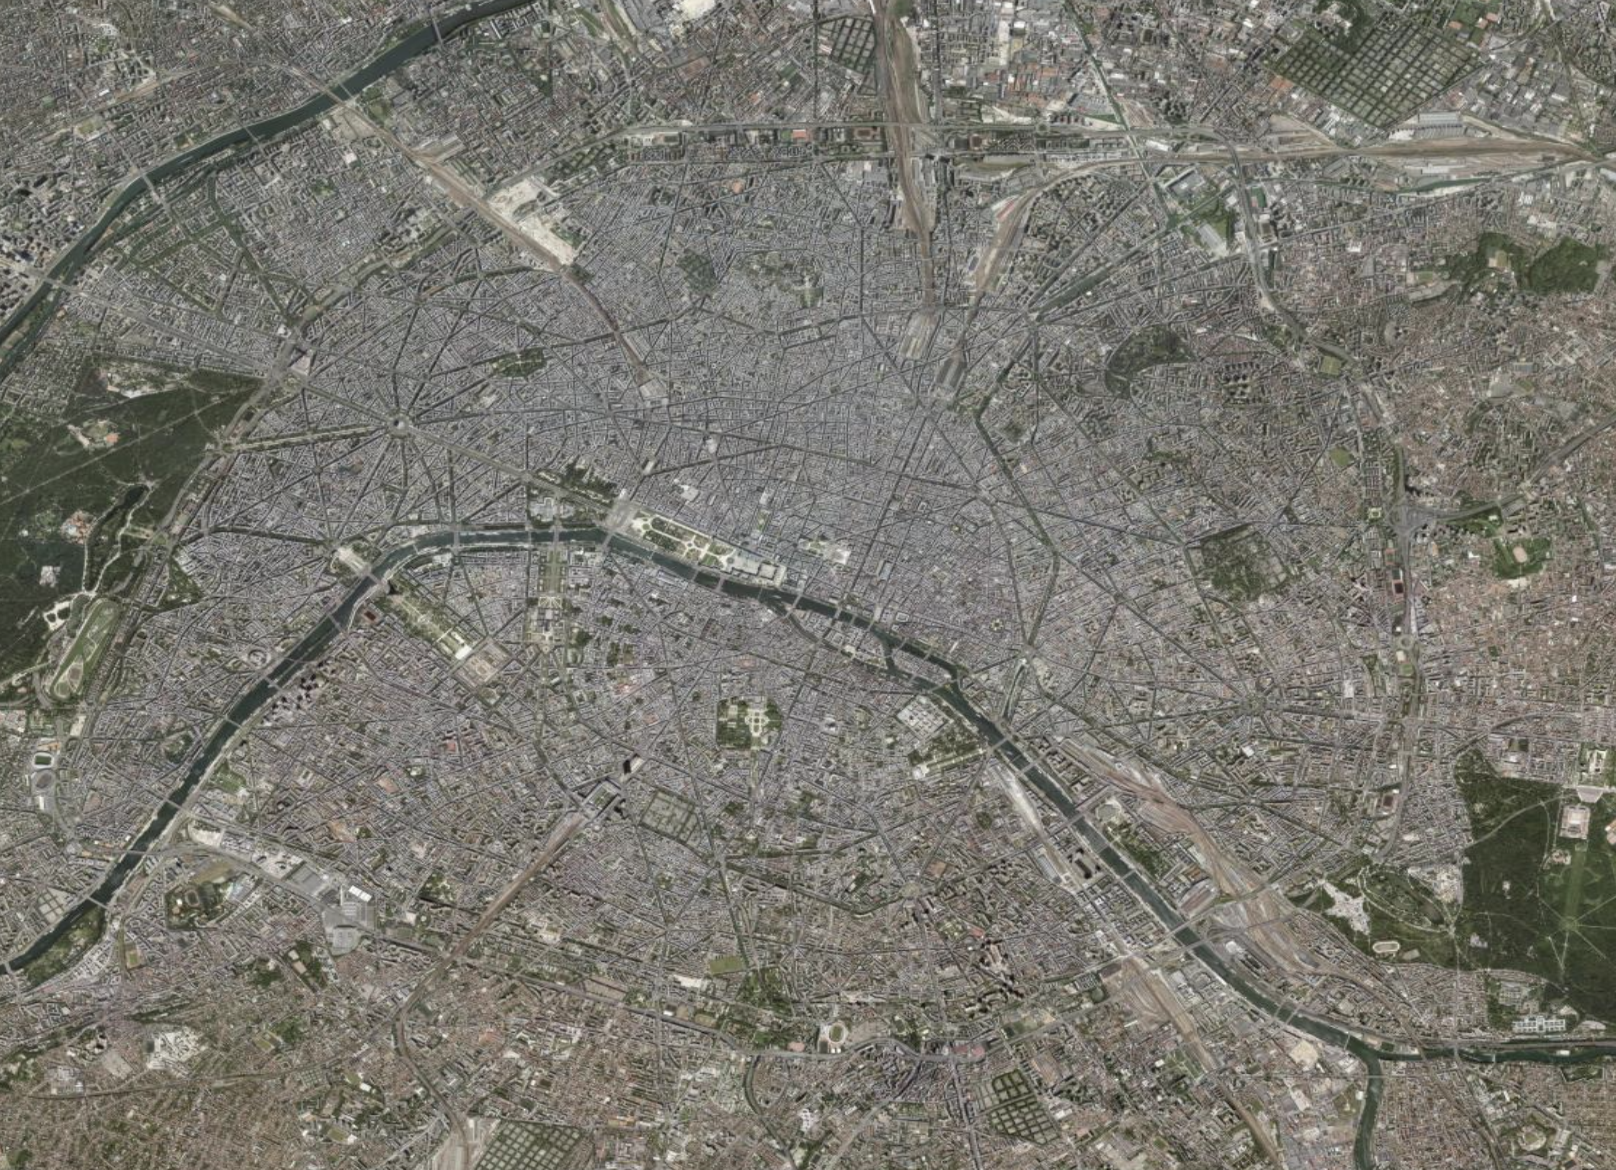
\includegraphics[width=0.9\textwidth]{figures/intro_paname}

\footnotesize\textit{Source: Geoportail}
}

\sframe{Complex processes of Urban Morphogenesis}{

\centering

% large bp
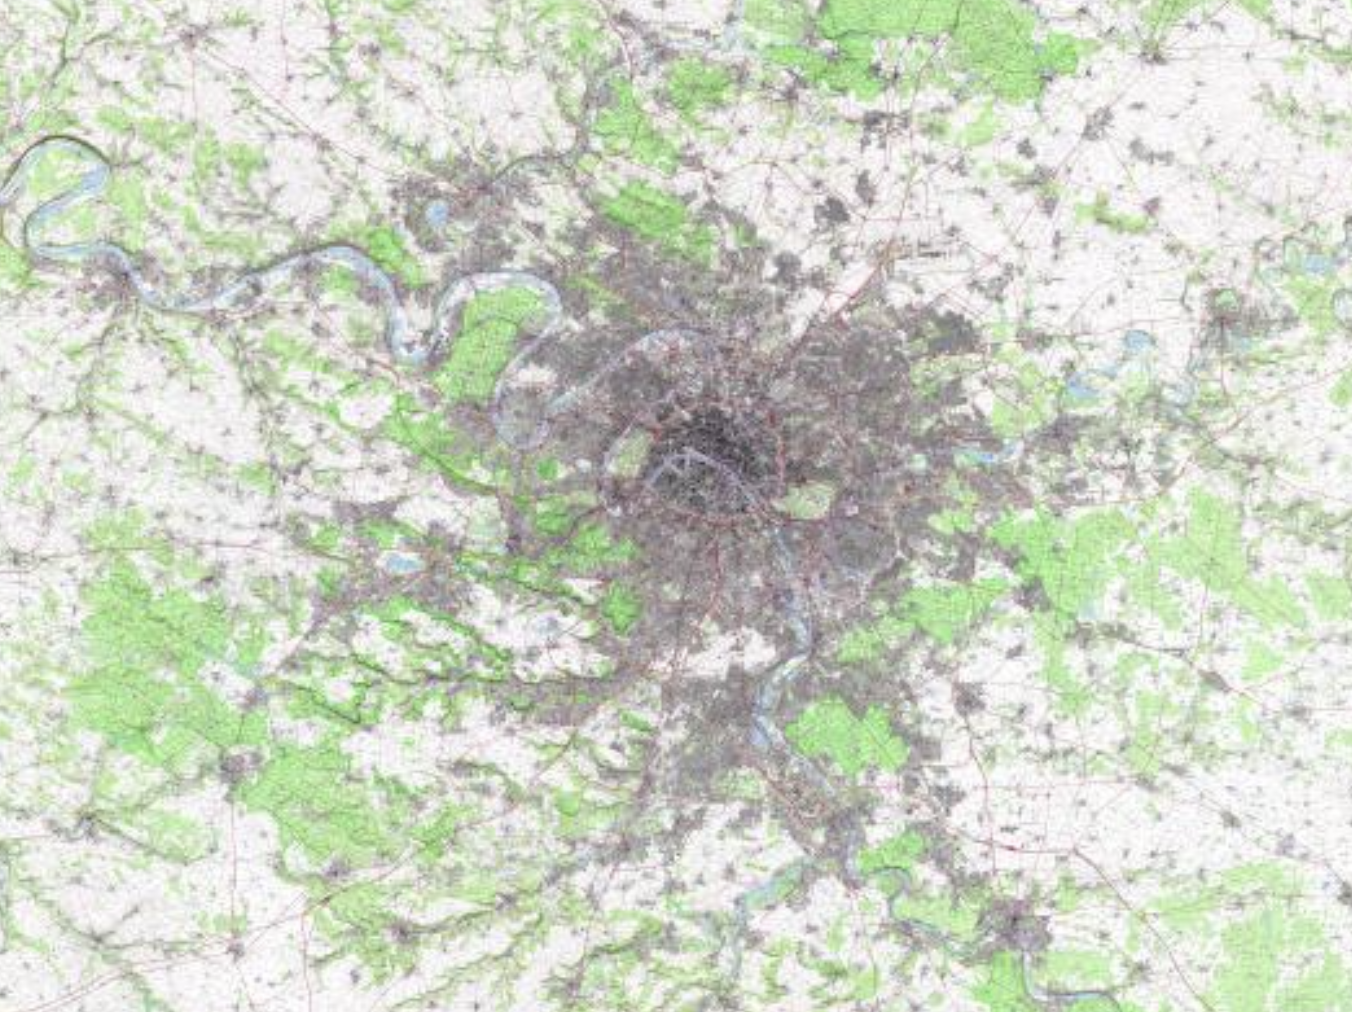
\includegraphics[width=0.9\textwidth]{figures/intro_bp}

\footnotesize\textit{Source: Geoportail}
}




\sframe{What is Morphogenesis ?}{

% illustrations : ants, geomorphology, neurons, self-assembly ; ARBOTRON ; paper nature aile avion
% all from netlogo library ? would be nice illustration of generative nature


\begin{columns}
\column{0.3\textwidth}
\centering
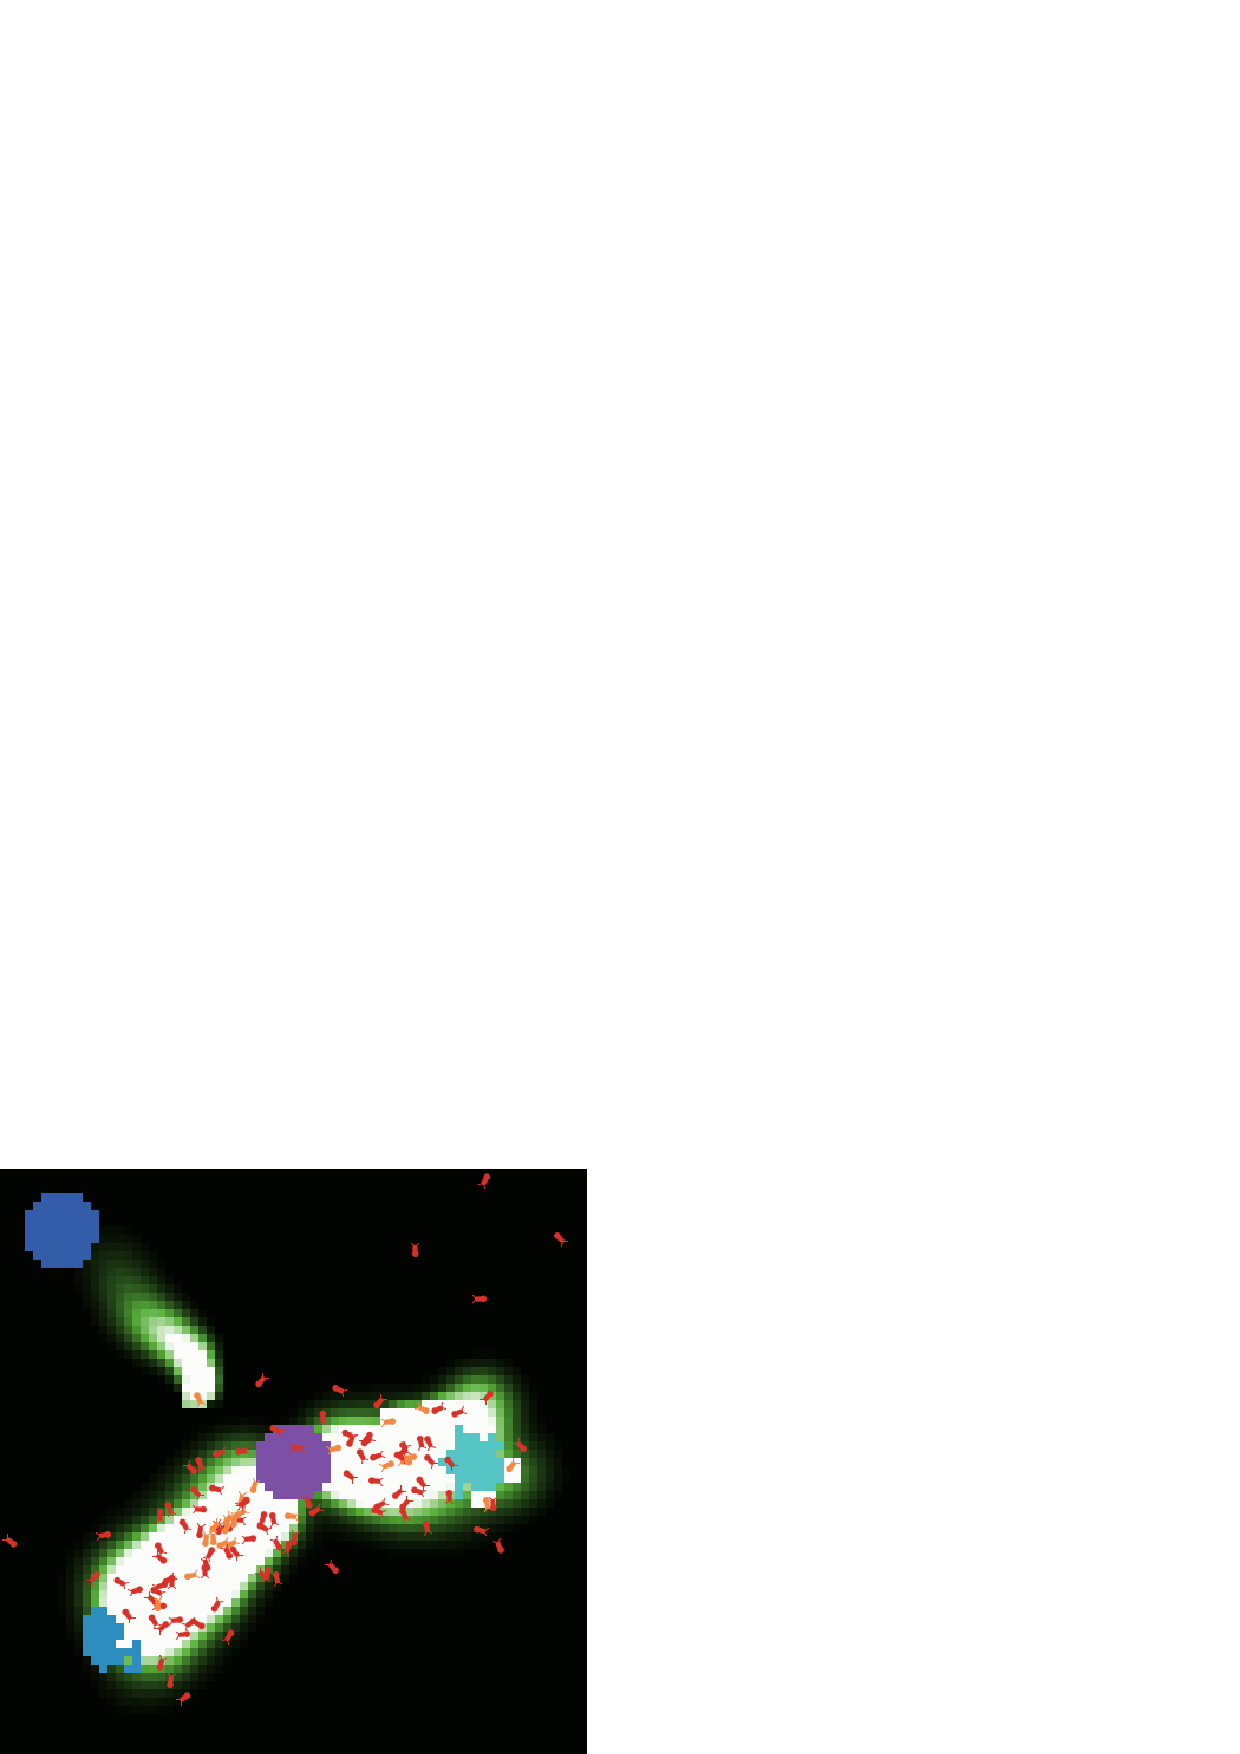
\includegraphics[width=\textwidth]{figures/intro_ants}\\\medskip
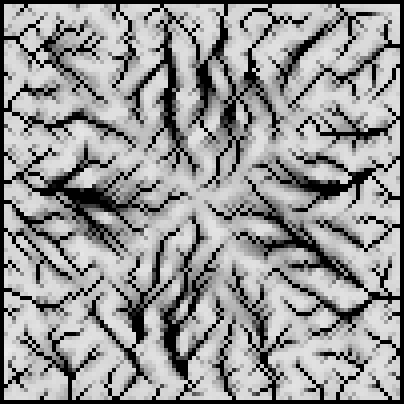
\includegraphics[width=\textwidth]{figures/intro_erosion}
\column{0.3\textwidth}
\centering
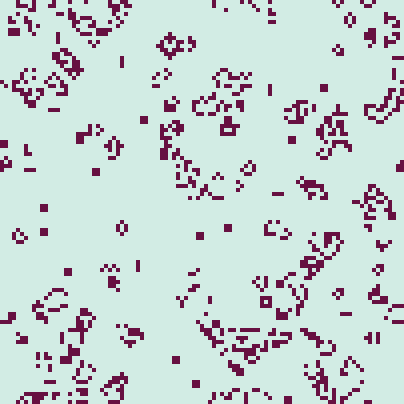
\includegraphics[width=\textwidth]{figures/intro_gameoflife}\\\vspace{0.7cm}
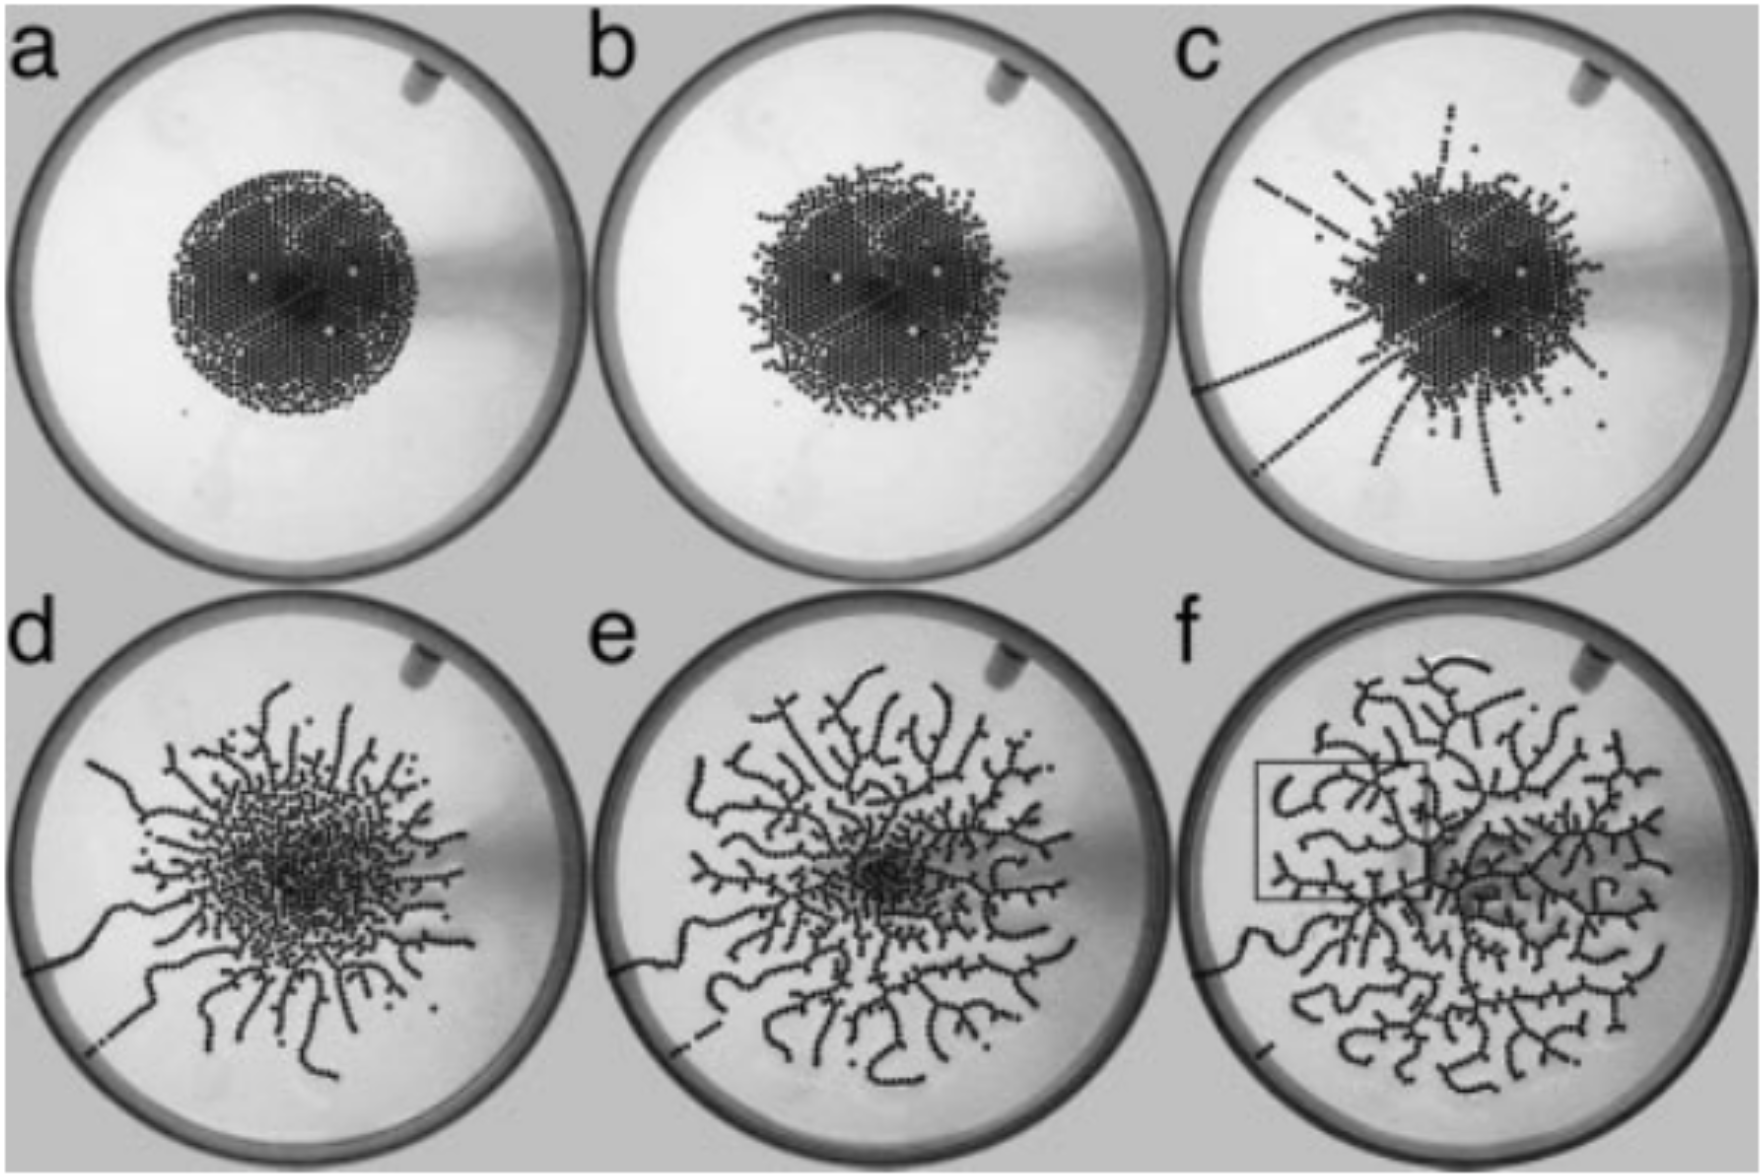
\includegraphics[width=\textwidth]{figures/intro_arbotron}
\column{0.35\textwidth}
\centering
\frame{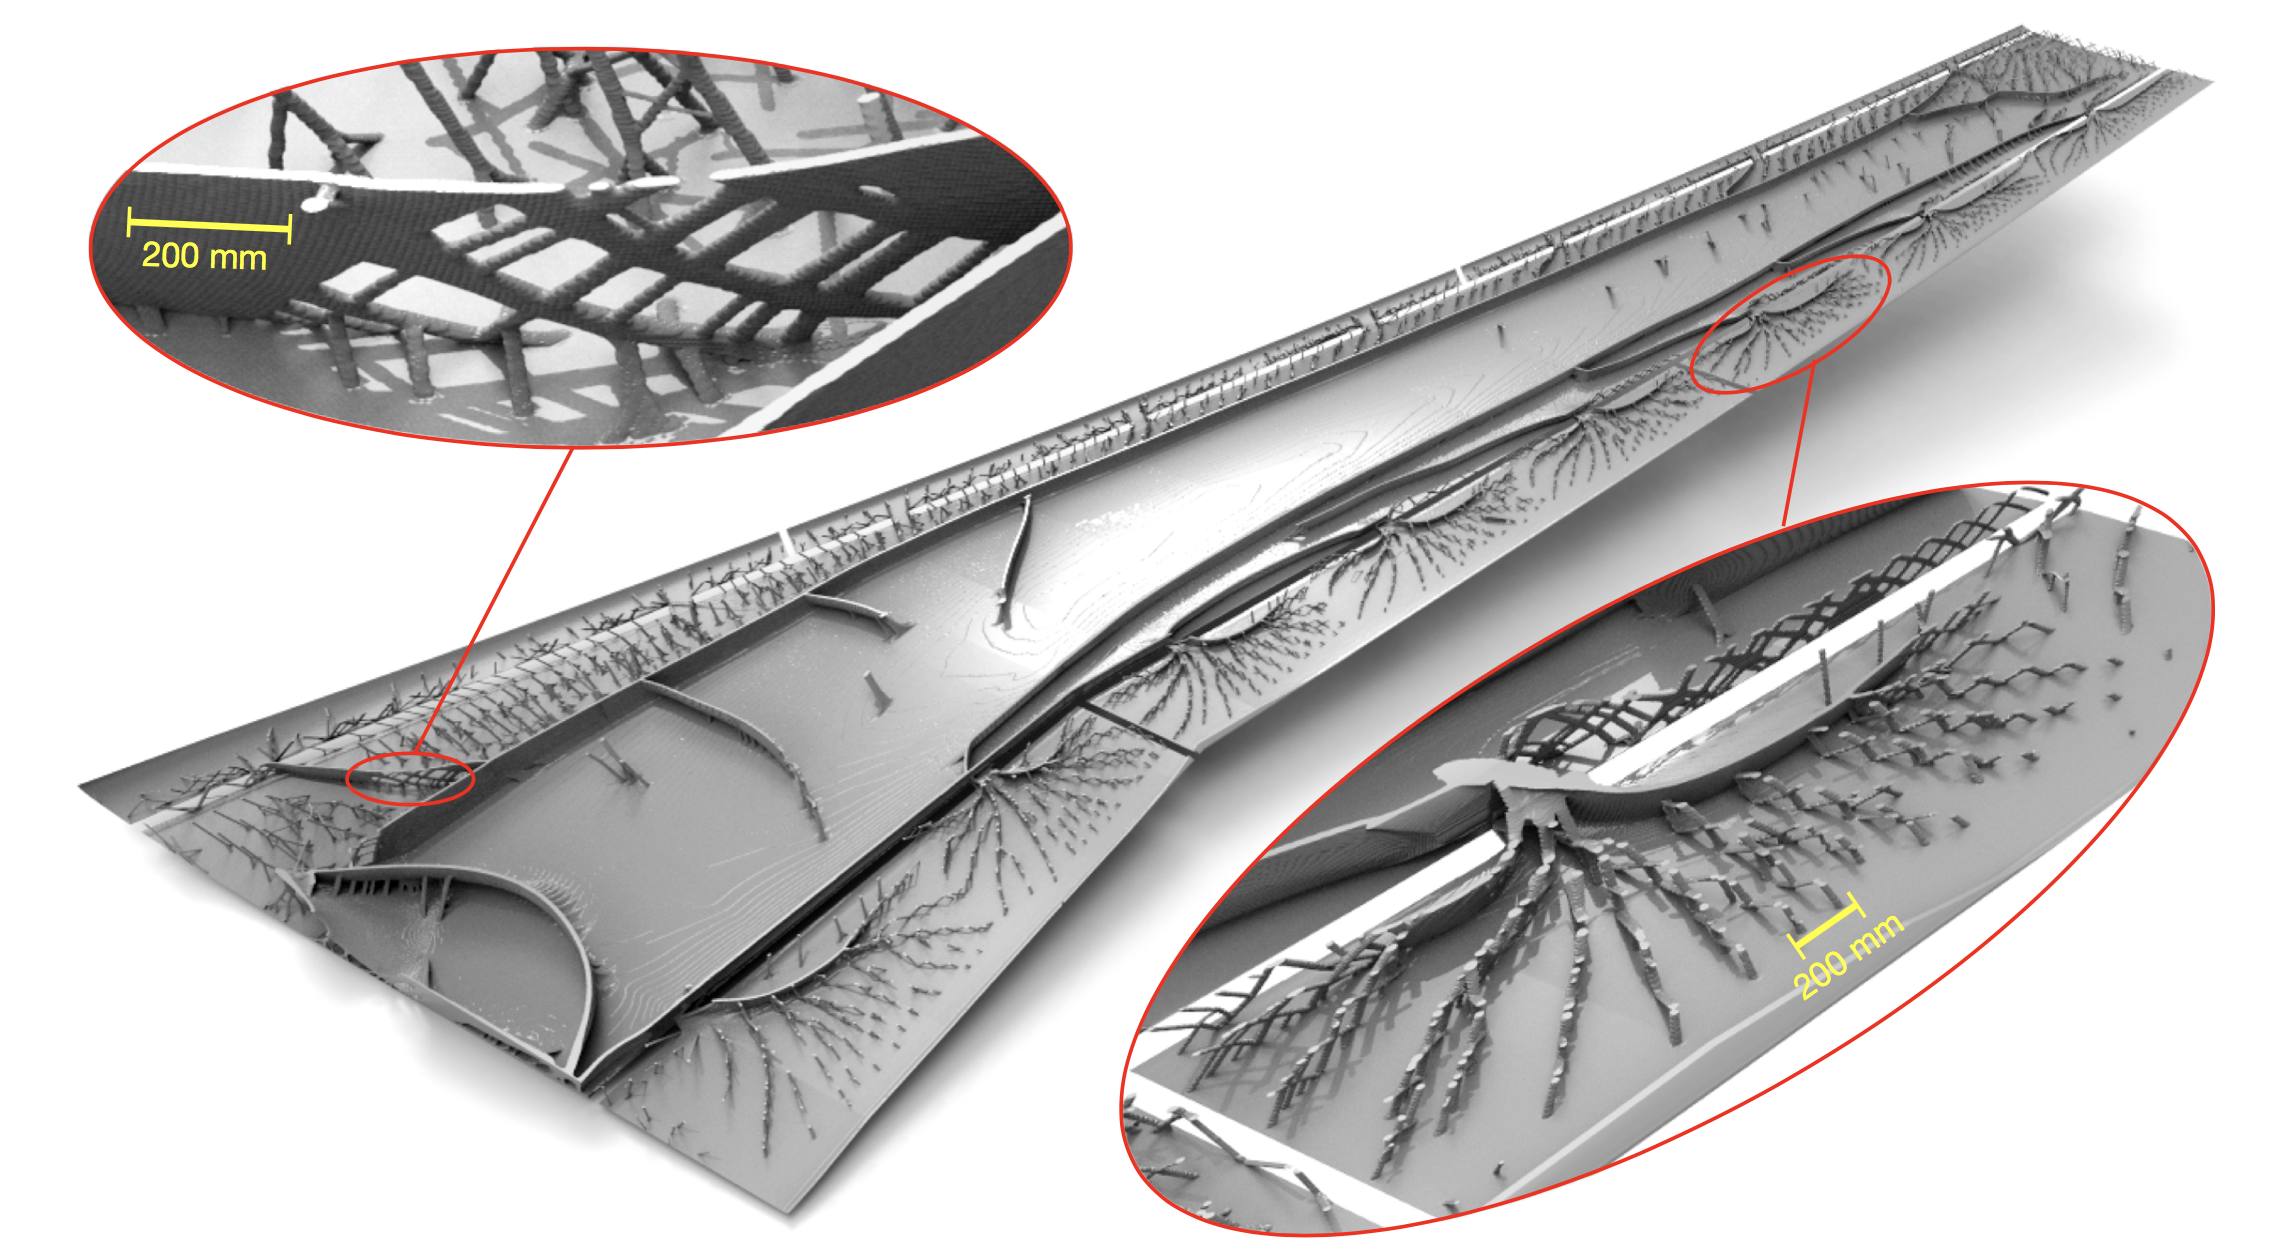
\includegraphics[width=\textwidth]{figures/intro_plane}}\\\medskip
\frame{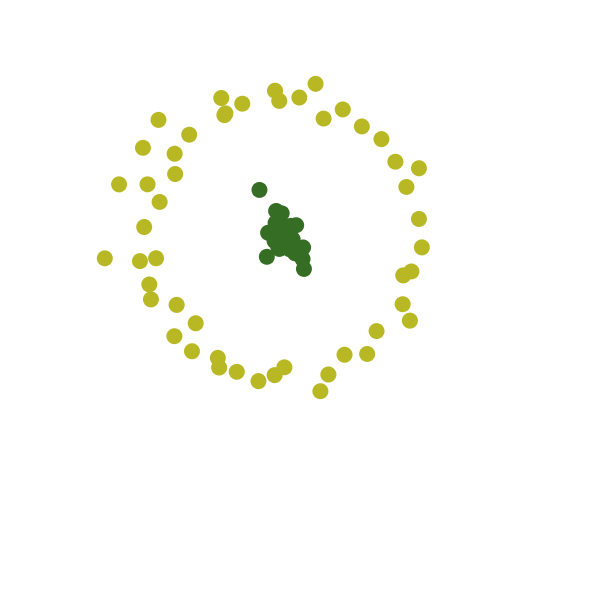
\includegraphics[width=\textwidth]{figures/intro_swarmchem}}
\end{columns}



\footnotesize\textit{Sources (in order by column). Ants, Erosion, Game of Life: NetLogo Library ; Arbotron \cite{jun2005formation}; Industrial design \cite{Aage:2017aa}; Swarm chemistry \cite{sayama2007decentralized}}
% sources : ants netlogo ; erosion netlogo ; arbotron 
%  inge : 

}



\sframe{Defining Morphogenesis}{

% precise notions and defs

\cite{antelope2016interdisciplinary}


Self-organization $\supsetneq$ Morphogenesis $\supsetneq$ Autopoiesis $\supsetneq$ Life

\bigskip

\begin{itemize}
\item Architecture links form and function~\cite{doursat2013review}
\item Emergence strength~\cite{bedau2002downward} diminishing with depth, whereas bifurcations increase~\cite{thom1974stabilite}
\end{itemize}


}



\sframe{Modeling Urban Morphogenesis}{

% why modeling, exemple of rbd

}


\sframe{A simple Aggregation-diffusion model}{

% model rationale and processes

}

\sframe{Model Formalization}{

% model formalization


}


\sframe{Generating Population Distributions}{

% examples : fig 2 of paper

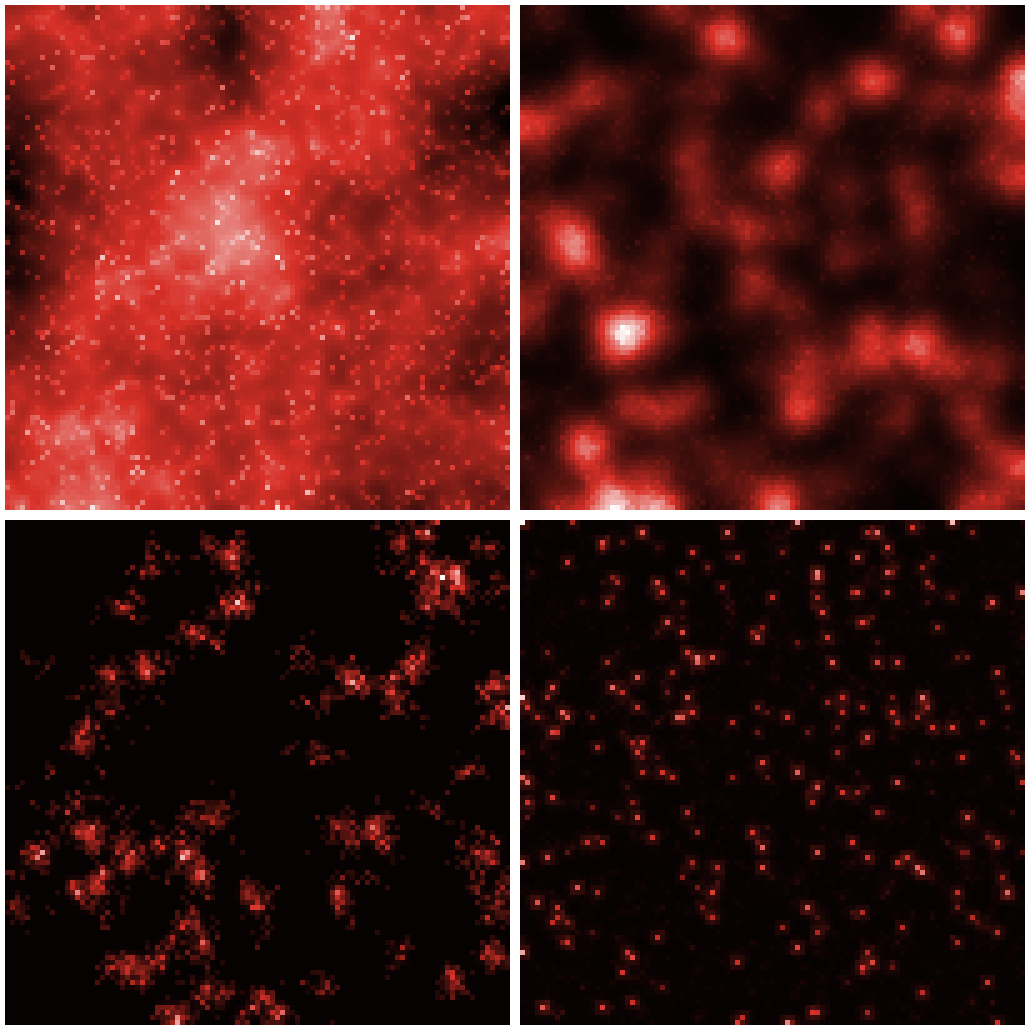
\includegraphics[height=\textheight]{figures/density_Fig2}


}


\sframe{Model behavior}{

}


\sframe{Model classification : PDE}{

}


\sframe{Path-dependence and frozen accidents}{

}


\sframe{Real Data}{

}



\sframe{Model Calibration}{

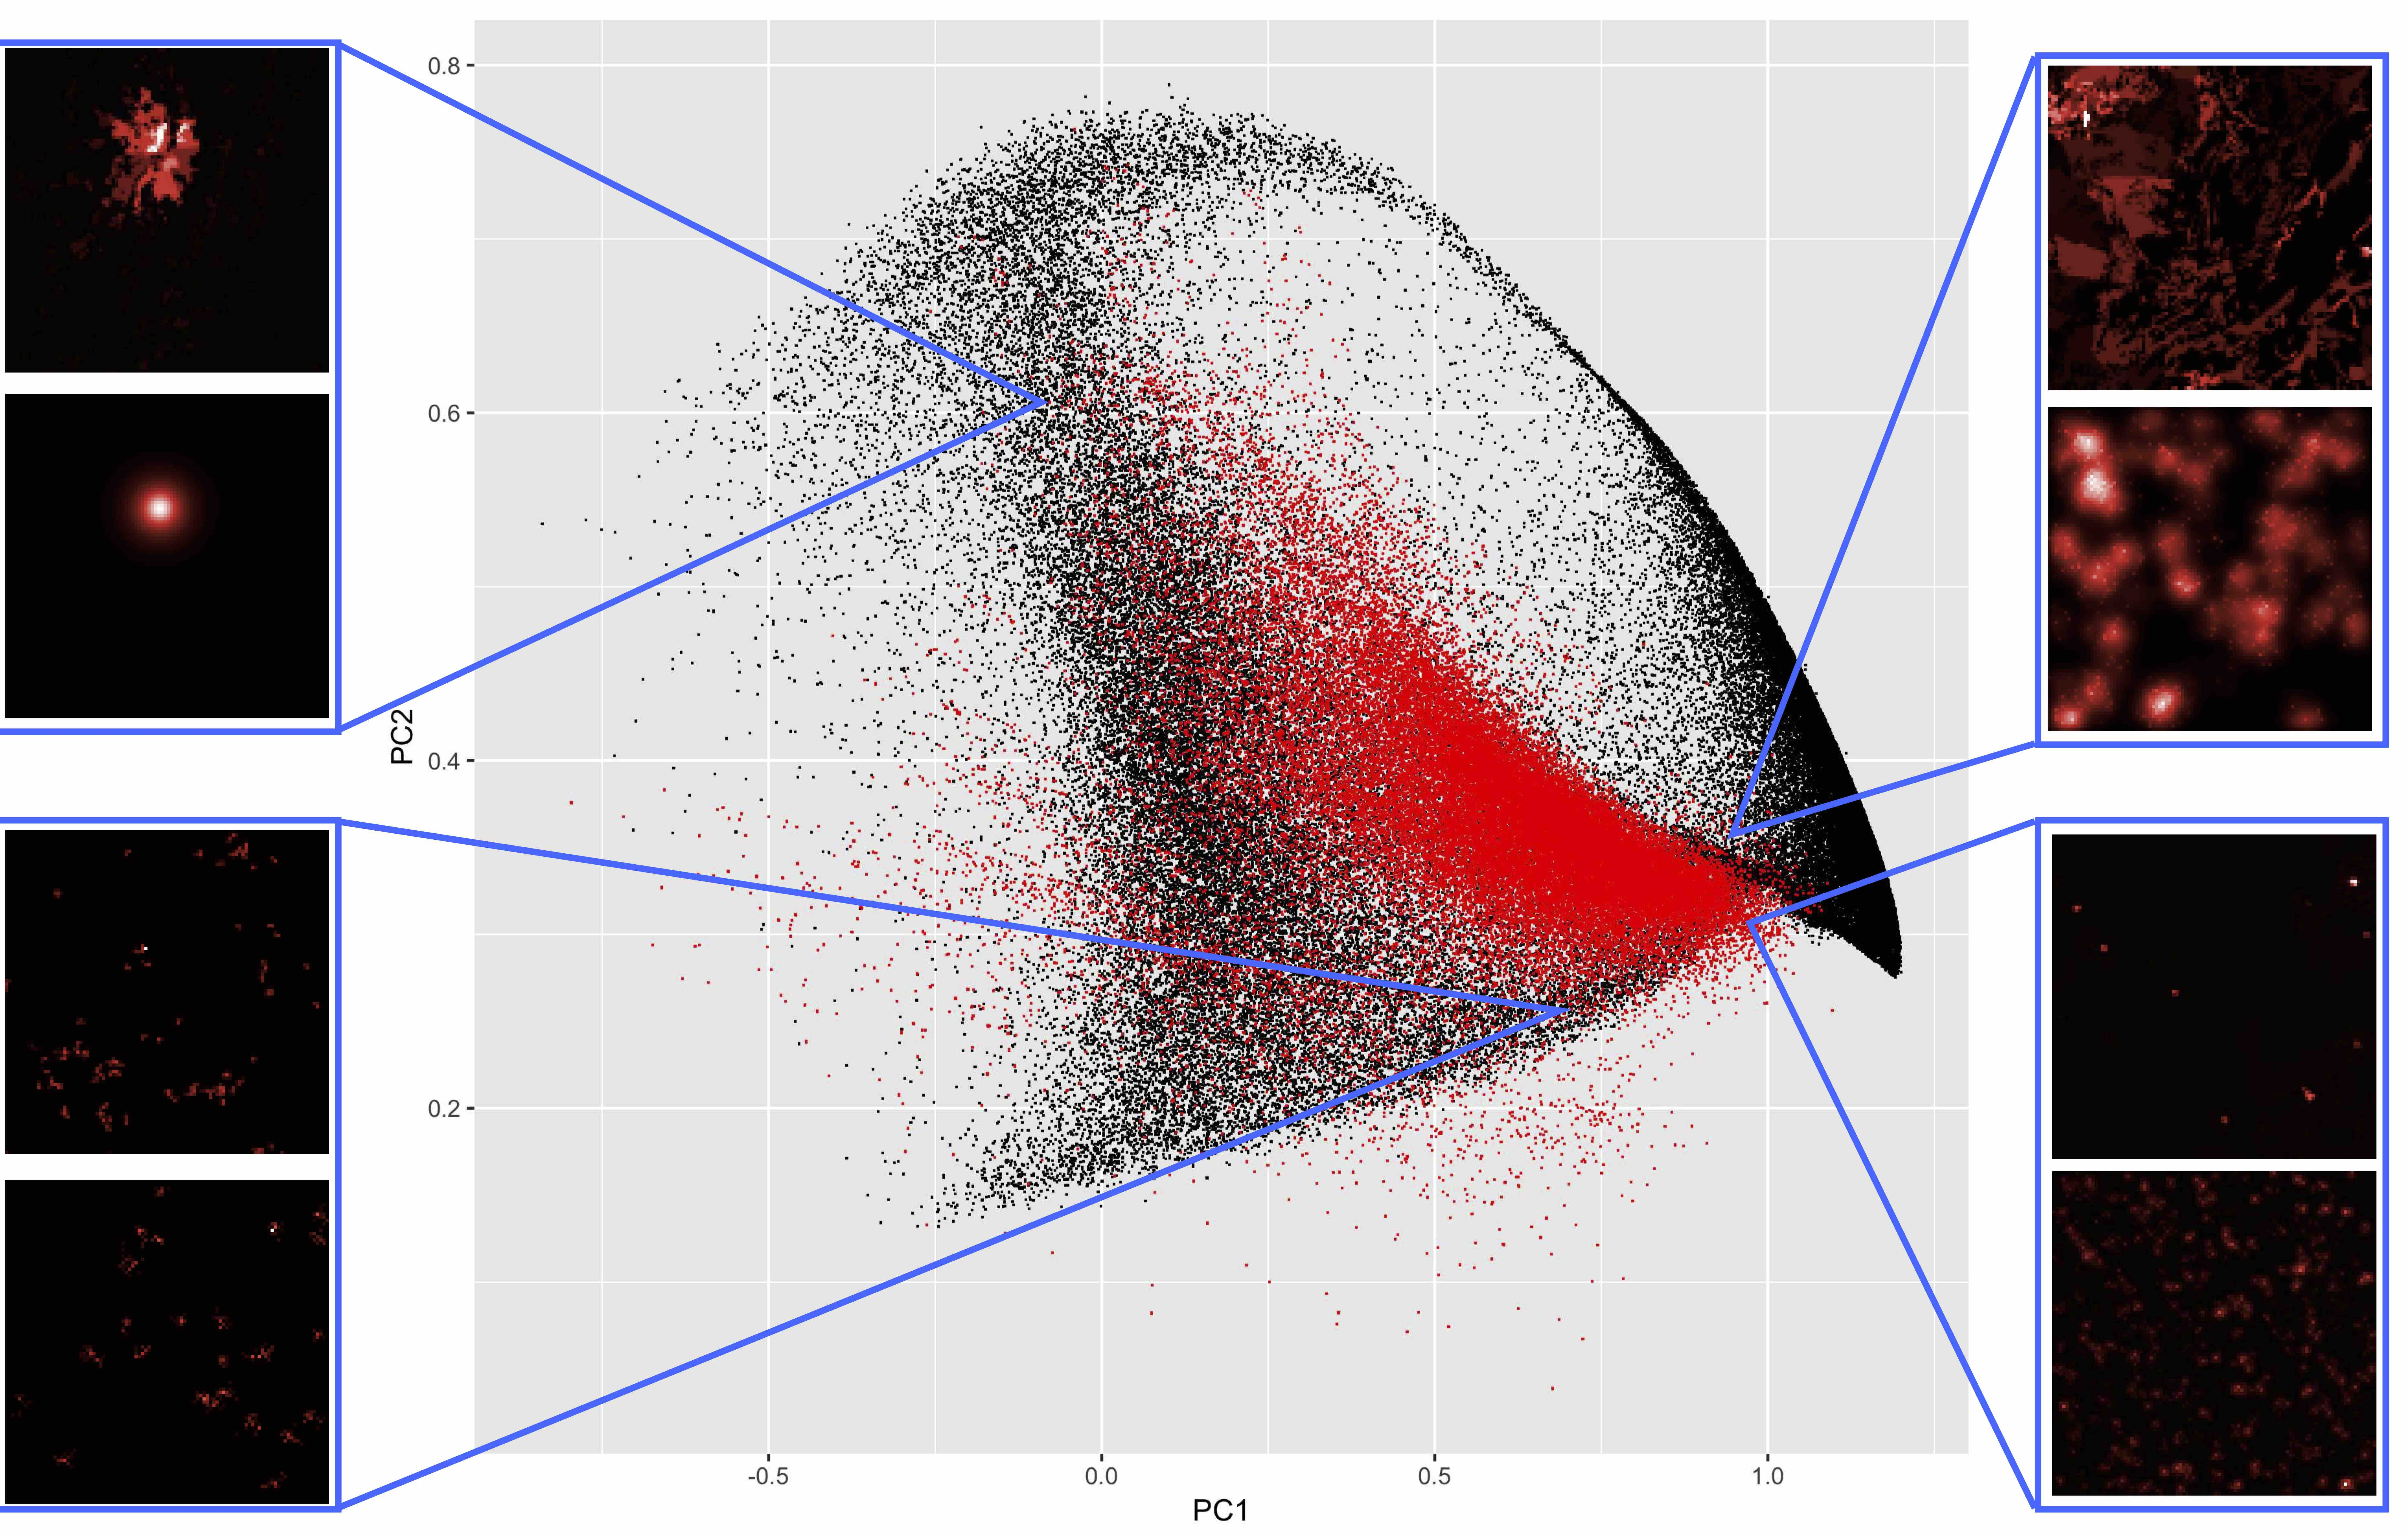
\includegraphics[width=\textwidth]{figures/density_synth}

}



\sframe{Including more complex processes ?}{

% transition : representation of territories

}


\sframe{Co-evolution of Transportation Networks and Territories}{

% qualitative slide
% eventually layus on literature with the cit nw ? maybe too much
% def. covevol : besoin coevol regimes, annexe
% idem macrocoevol en annexe


}



\sframe{A Morphogenesis Model of co-evolution}{

\justify

\vspace{-1cm}

$\rightarrow$ Coupled grid population distribution and vector transportation network, following the core of \cite{raimbault2014hybrid}

\medskip

$\rightarrow$ Local morphological and functional variables determine a patch-value, driving new population attribution through preferential attachment ; combined to population diffusion (aggregation-diffusion processes studied in \cite{2017arXiv170806743R})

\medskip

$\rightarrow$ Network growth is also driven by morphological, functional and local network measures, following diverse heuristics corresponding to different processes (multi-modeling)

\bigskip
\bigskip

\textit{Local variables and network properties induce feedback on both, thus a strong coupling capturing the \textbf{co-evolution}}

}



\sframe{Model : Specification}{

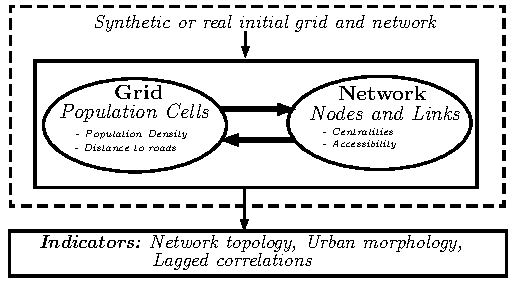
\includegraphics[width=\textwidth]{figures/coevol_mesocoevol}

}



\sframe{Network Generation}{

At fixed time steps :

\begin{enumerate}
	\item Add new nodes preferentially to new population and connect them
	\item \justify Variable heuristic for new links, among: nothing, random, gravity-based deterministic breakdown, gravity-based random breakdown (from \cite{schmitt2014modelisation}), cost-benefits (from \cite{louf2013emergence}), biological network generation (based on \cite{tero2010rules})
\end{enumerate}

\medskip

\centering

\frame{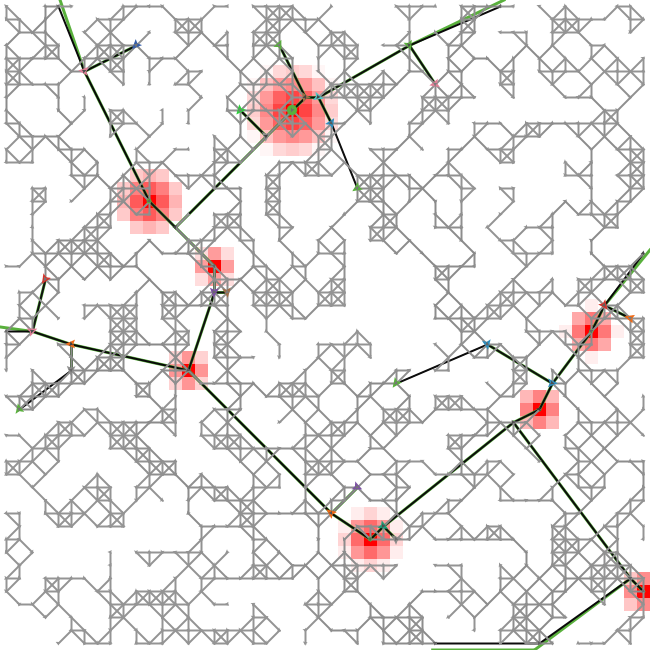
\includegraphics[height=0.31\textwidth]{figures/coevol_example-bio-process-1}}\hspace{0.2cm}
\frame{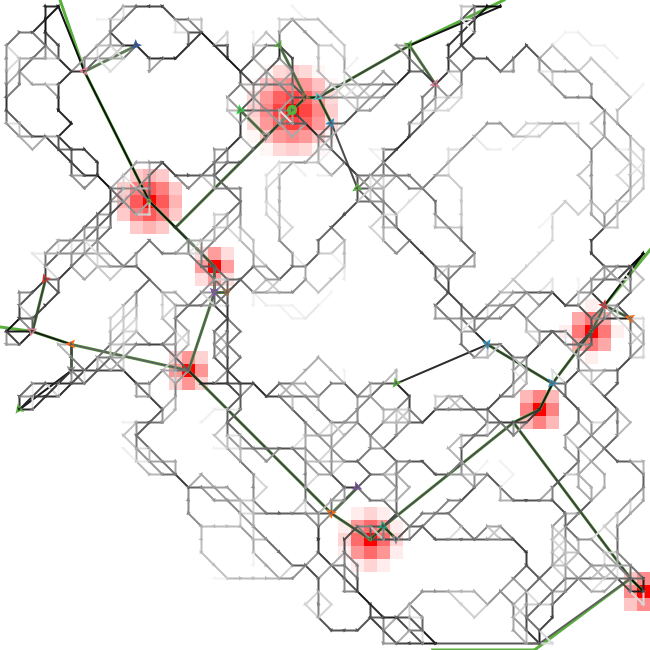
\includegraphics[height=0.31\textwidth]{figures/coevol_example-bio-process-1-tick80}}

\footnotesize

\textit{Intermediate stage for biological network generation}

}




\sframe{Generated Urban Shapes: Urban Form}{

\centering

\frame{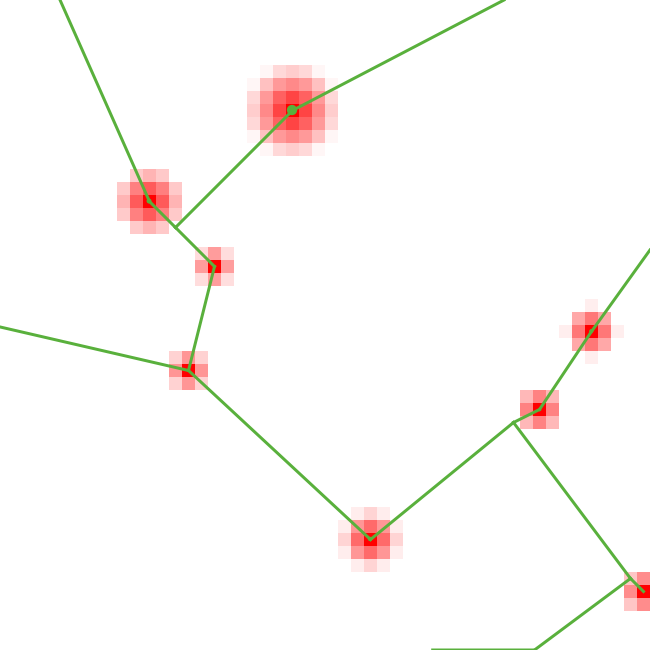
\includegraphics[width=0.28\textwidth]{figures/coevol_example_synthsetup}}\hspace{0.1cm}
\frame{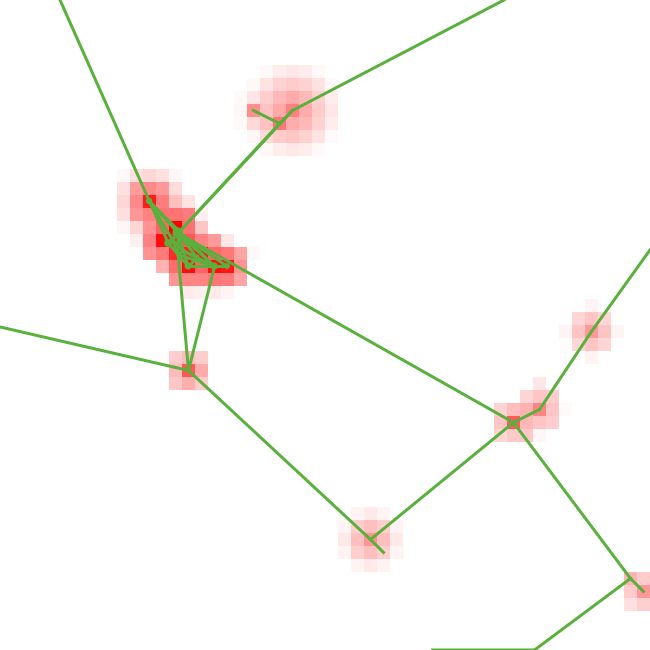
\includegraphics[width=0.28\textwidth]{figures/coevol_example_form-accessonly}}\hspace{0.1cm}
\frame{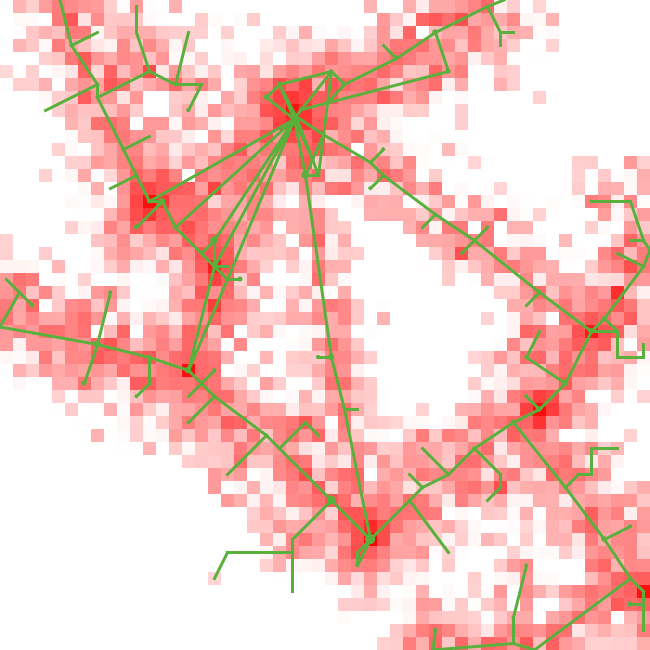
\includegraphics[width=0.28\textwidth]{figures/coevol_example_form-droadonly}}\\\vspace{0.1cm}
\frame{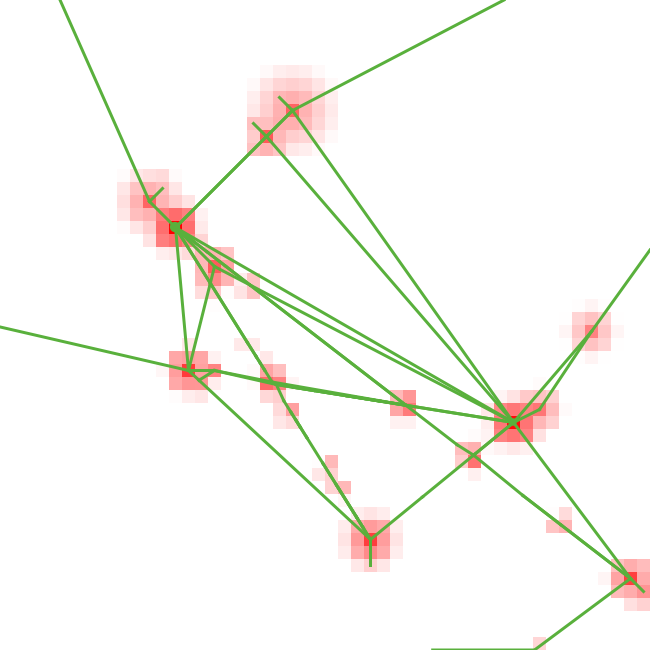
\includegraphics[width=0.28\textwidth]{figures/coevol_example_form-bwonly}}\hspace{0.1cm}
\frame{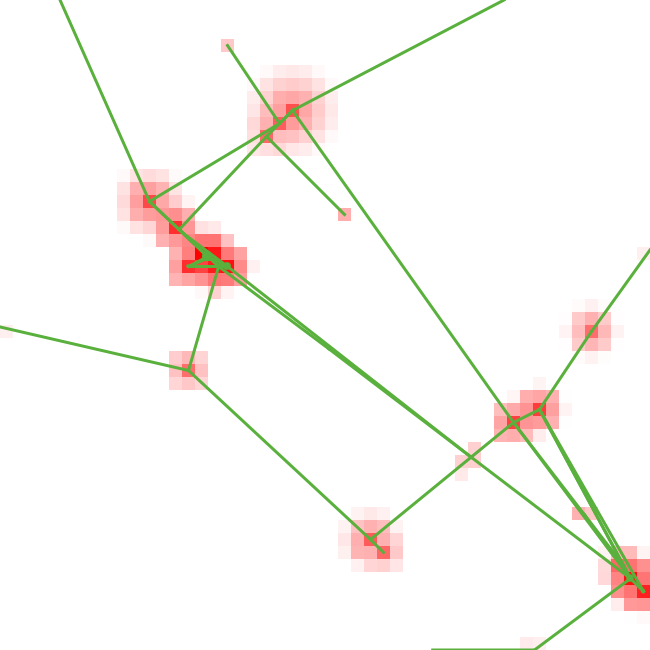
\includegraphics[width=0.28\textwidth]{figures/coevol_example_form-closenessonly}}\hspace{0.1cm}
\frame{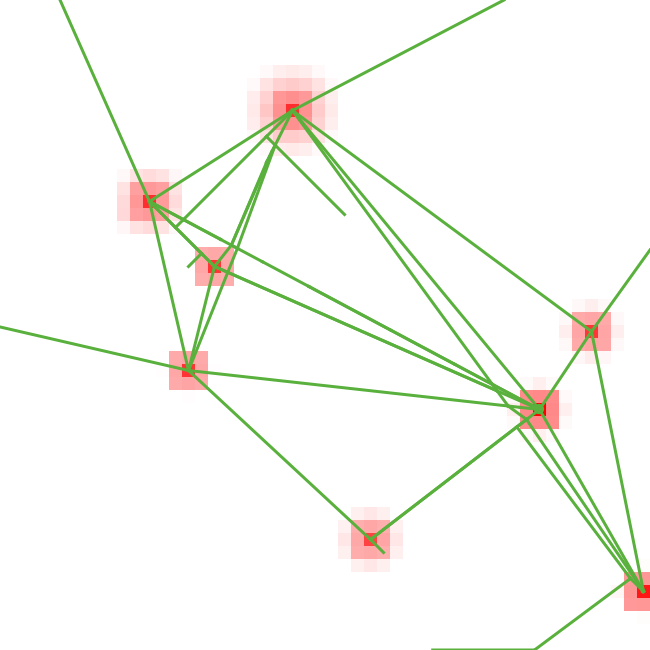
\includegraphics[width=0.28\textwidth]{figures/coevol_example_form-poponly}}

\footnotesize\textit{In order: setup; accessibility driven; road distance driven; betweenness driven; closeness driven; population driven.}

}






\sframe{Generated Urban Shapes: Network}{


\centering

\frame{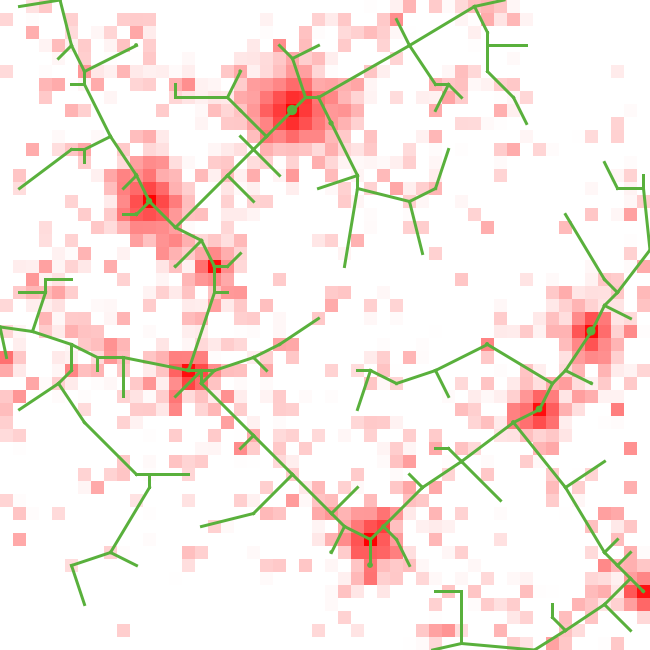
\includegraphics[width=0.28\textwidth]{figures/coevol_example_nw-connection}}\hspace{0.1cm}
\frame{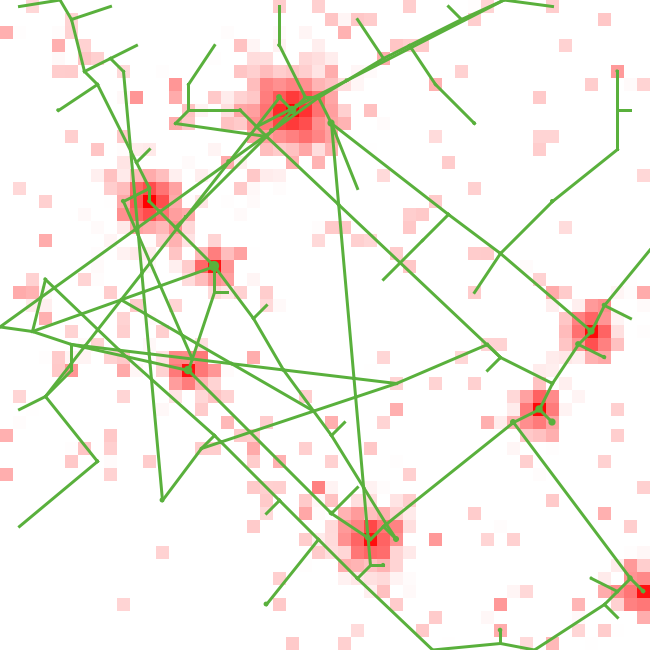
\includegraphics[width=0.28\textwidth]{figures/coevol_example_nw-random}}\hspace{0.1cm}
\frame{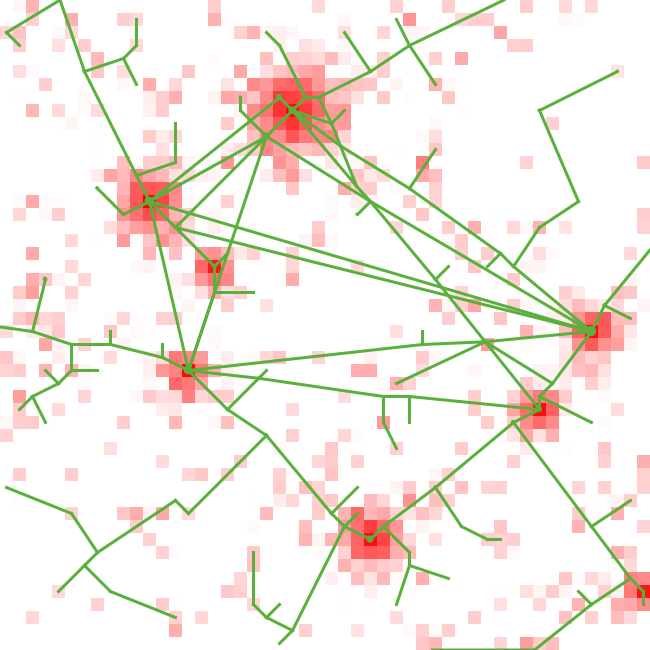
\includegraphics[width=0.28\textwidth]{figures/coevol_example_nw-gravity}}\\\vspace{0.1cm}
\frame{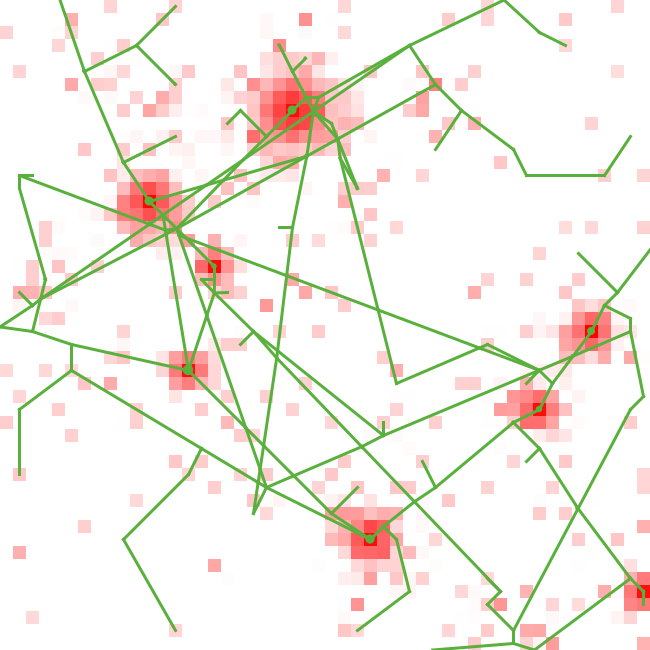
\includegraphics[width=0.28\textwidth]{figures/coevol_example_nw-rndbrkdwn}}\hspace{0.1cm}
\frame{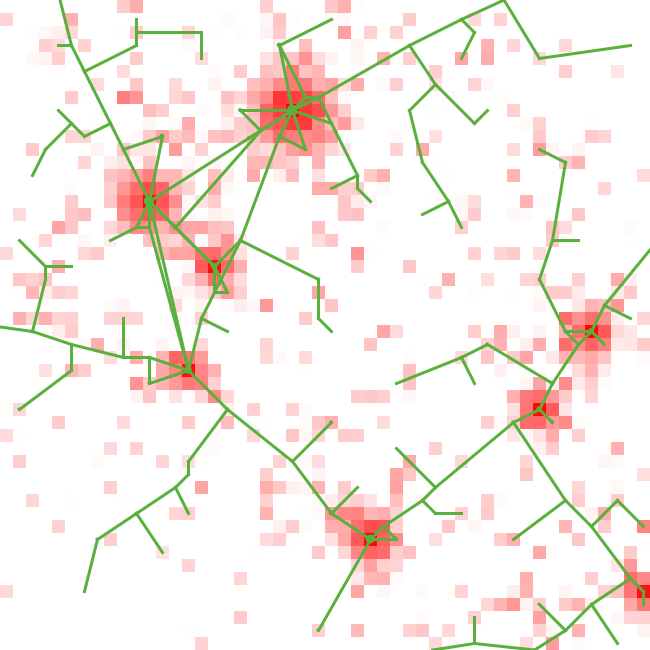
\includegraphics[width=0.28\textwidth]{figures/coevol_example_nw-cost}}\hspace{0.1cm}
\frame{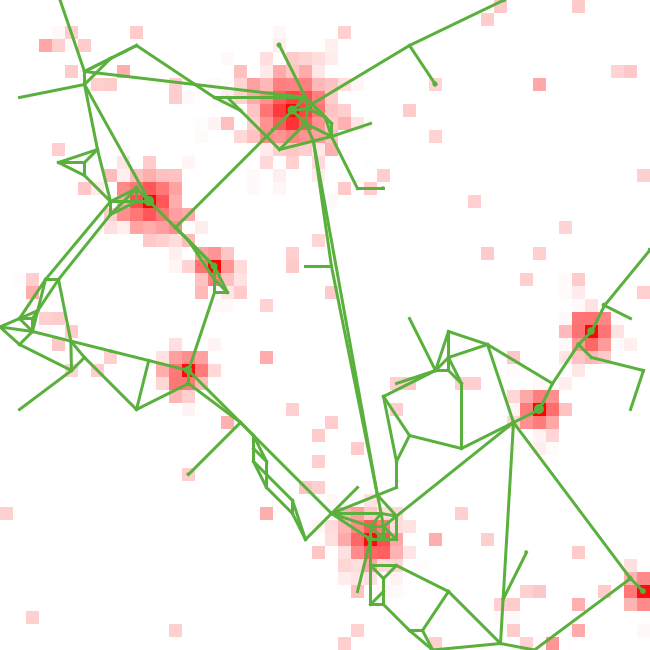
\includegraphics[width=0.28\textwidth]{figures/coevol_example_nw-bio}}

\footnotesize\textit{In order: connection; random; deterministic breakdown; random breakdown; cost-driven; biological.}

}



\sframe{Results : Network Heuristics}{

\justify

\textit{Comparison of feasible space for network indicators with fixed density}

\bigskip

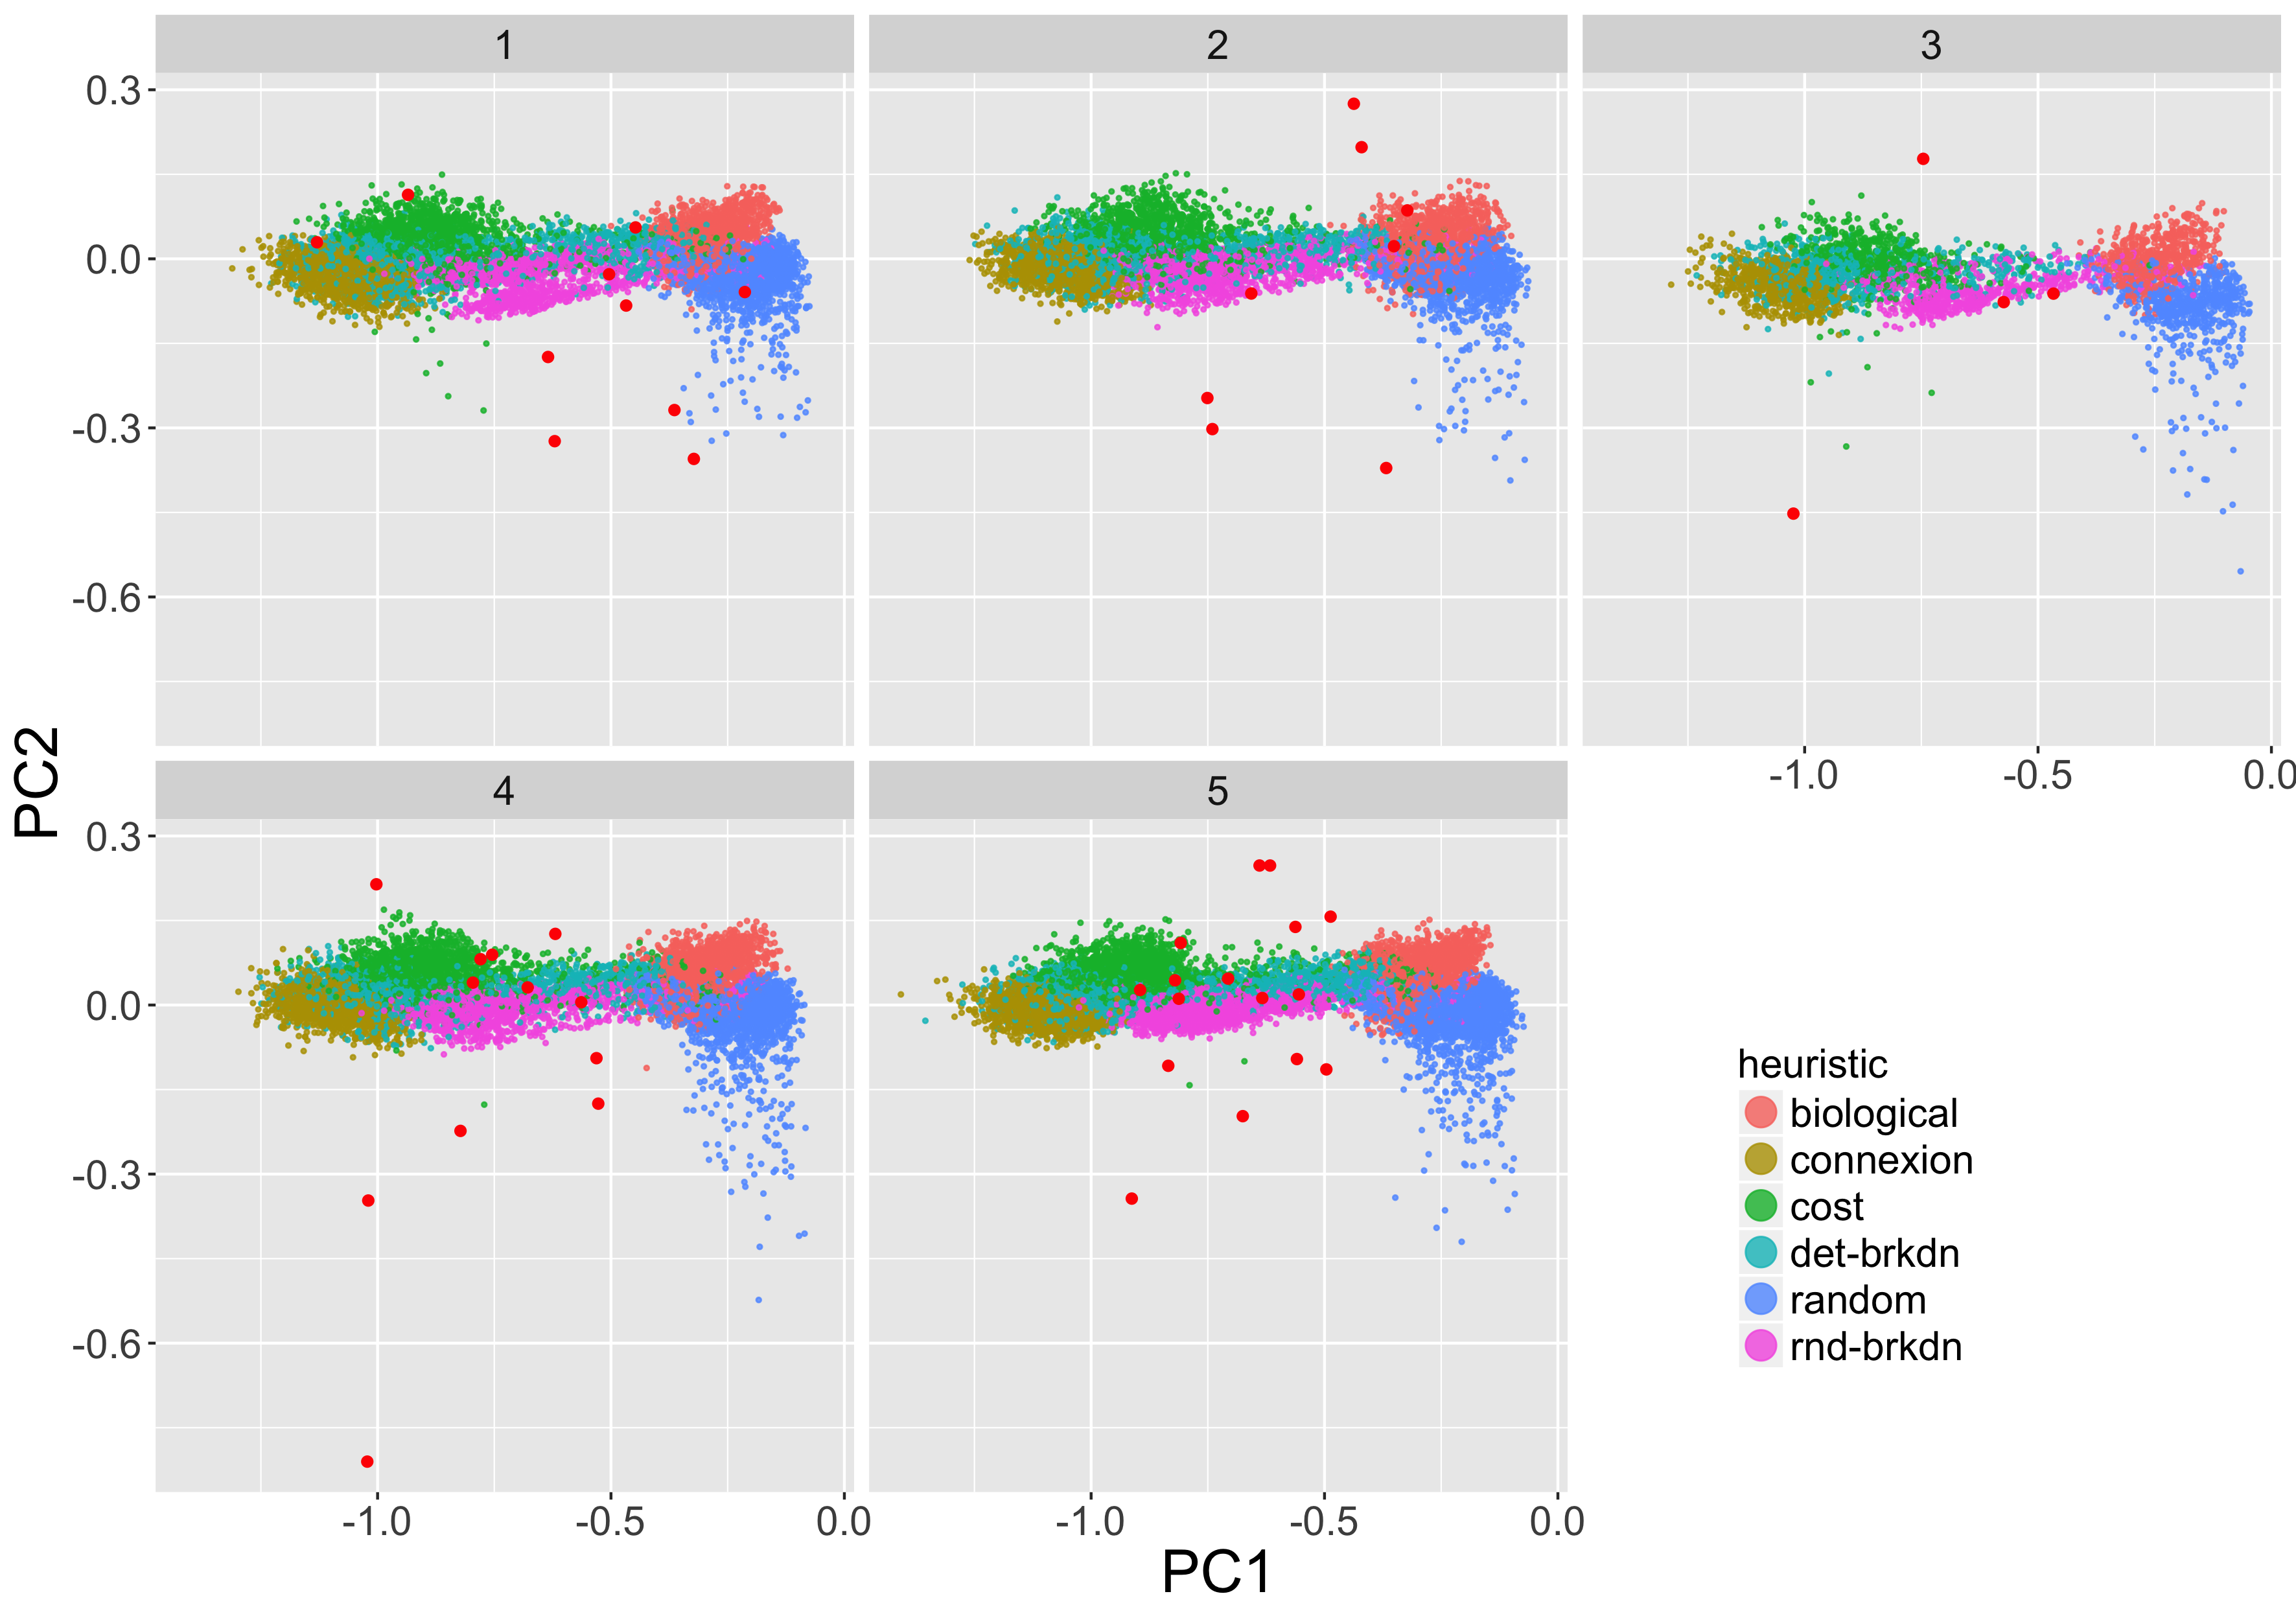
\includegraphics[width=0.52\textwidth,height=0.6\textheight]{figures/coevol_feasible_space_withreal_pca_bymorph}
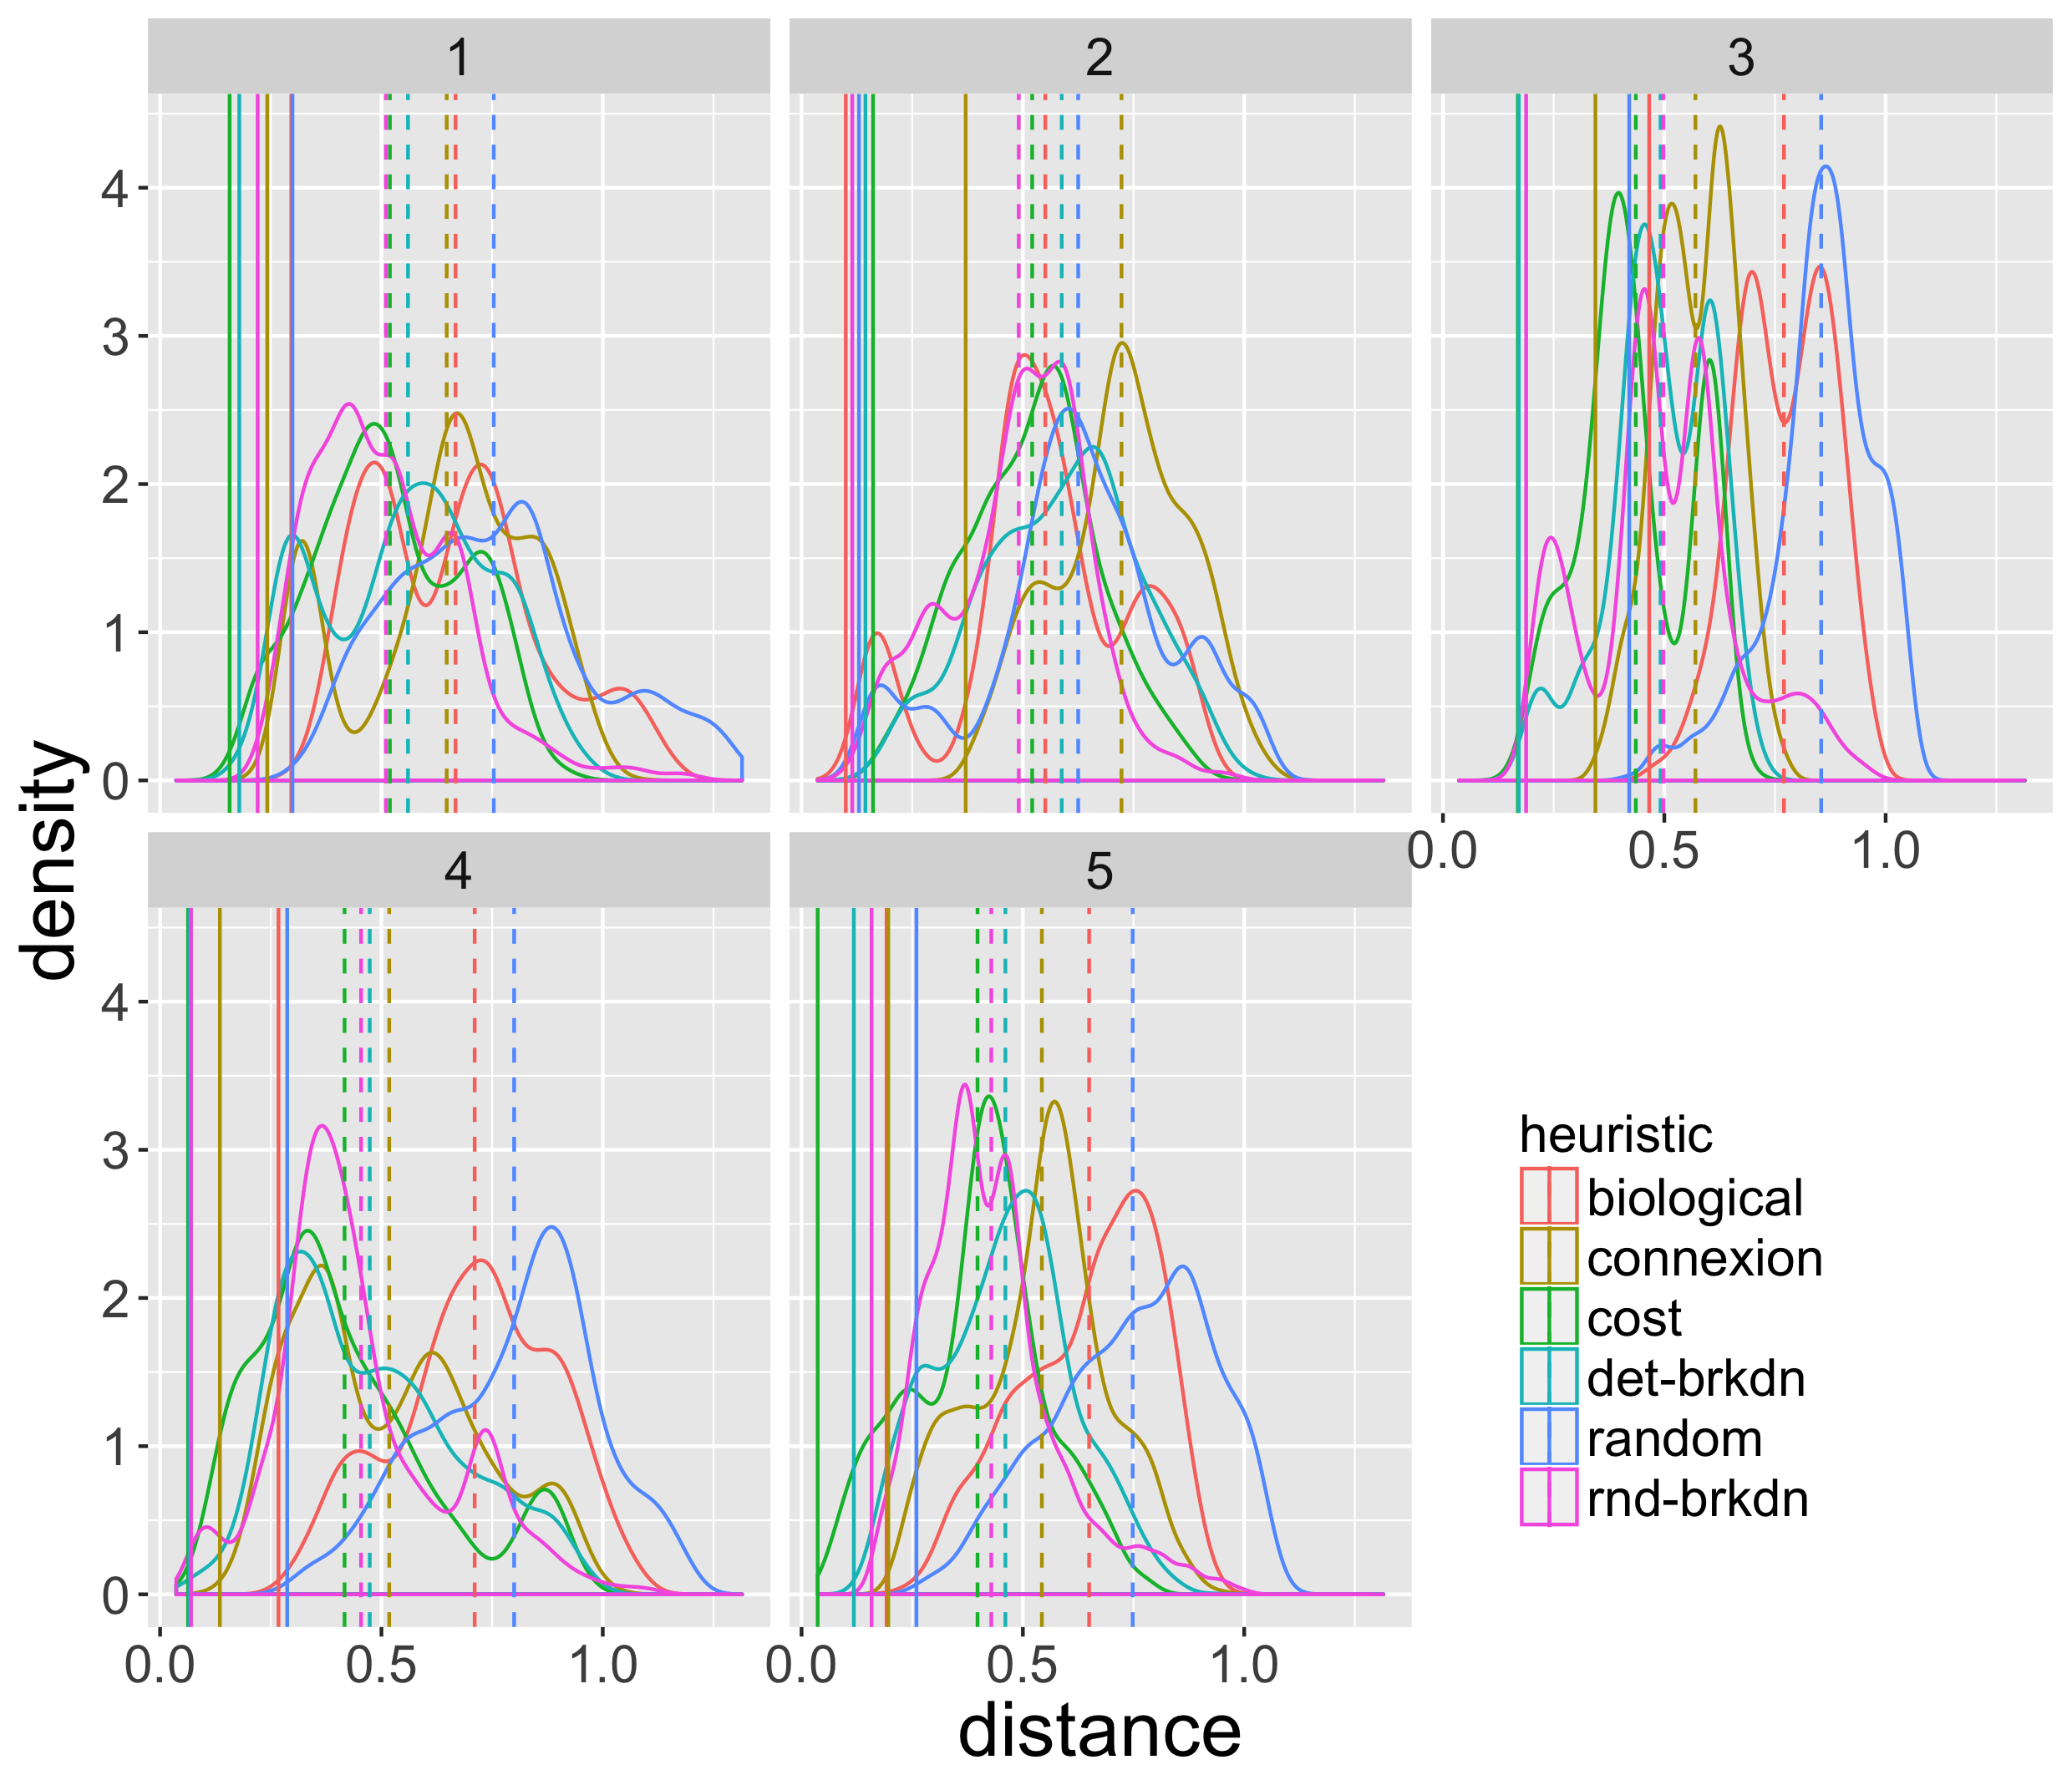
\includegraphics[width=0.43\textwidth,height=0.6\textheight]{figures/coevol_distance_real_bymorph}

\footnotesize

\textit{(Left) Feasible spaces by morphological class and network heuristic; (Right) Distribution of distances to topologies of real networks}

}


\sframe{Results : Calibration}{

\justify

\vspace{-0.5cm}

Calibration (model explored with OpenMole~\cite{reuillon2013openmole}, $\sim 10^6$ model runs) at the first order on morphological and topological objectives, and on correlations matrices.

\bigskip

\begin{columns}
\column{0.4\textwidth}
\centering
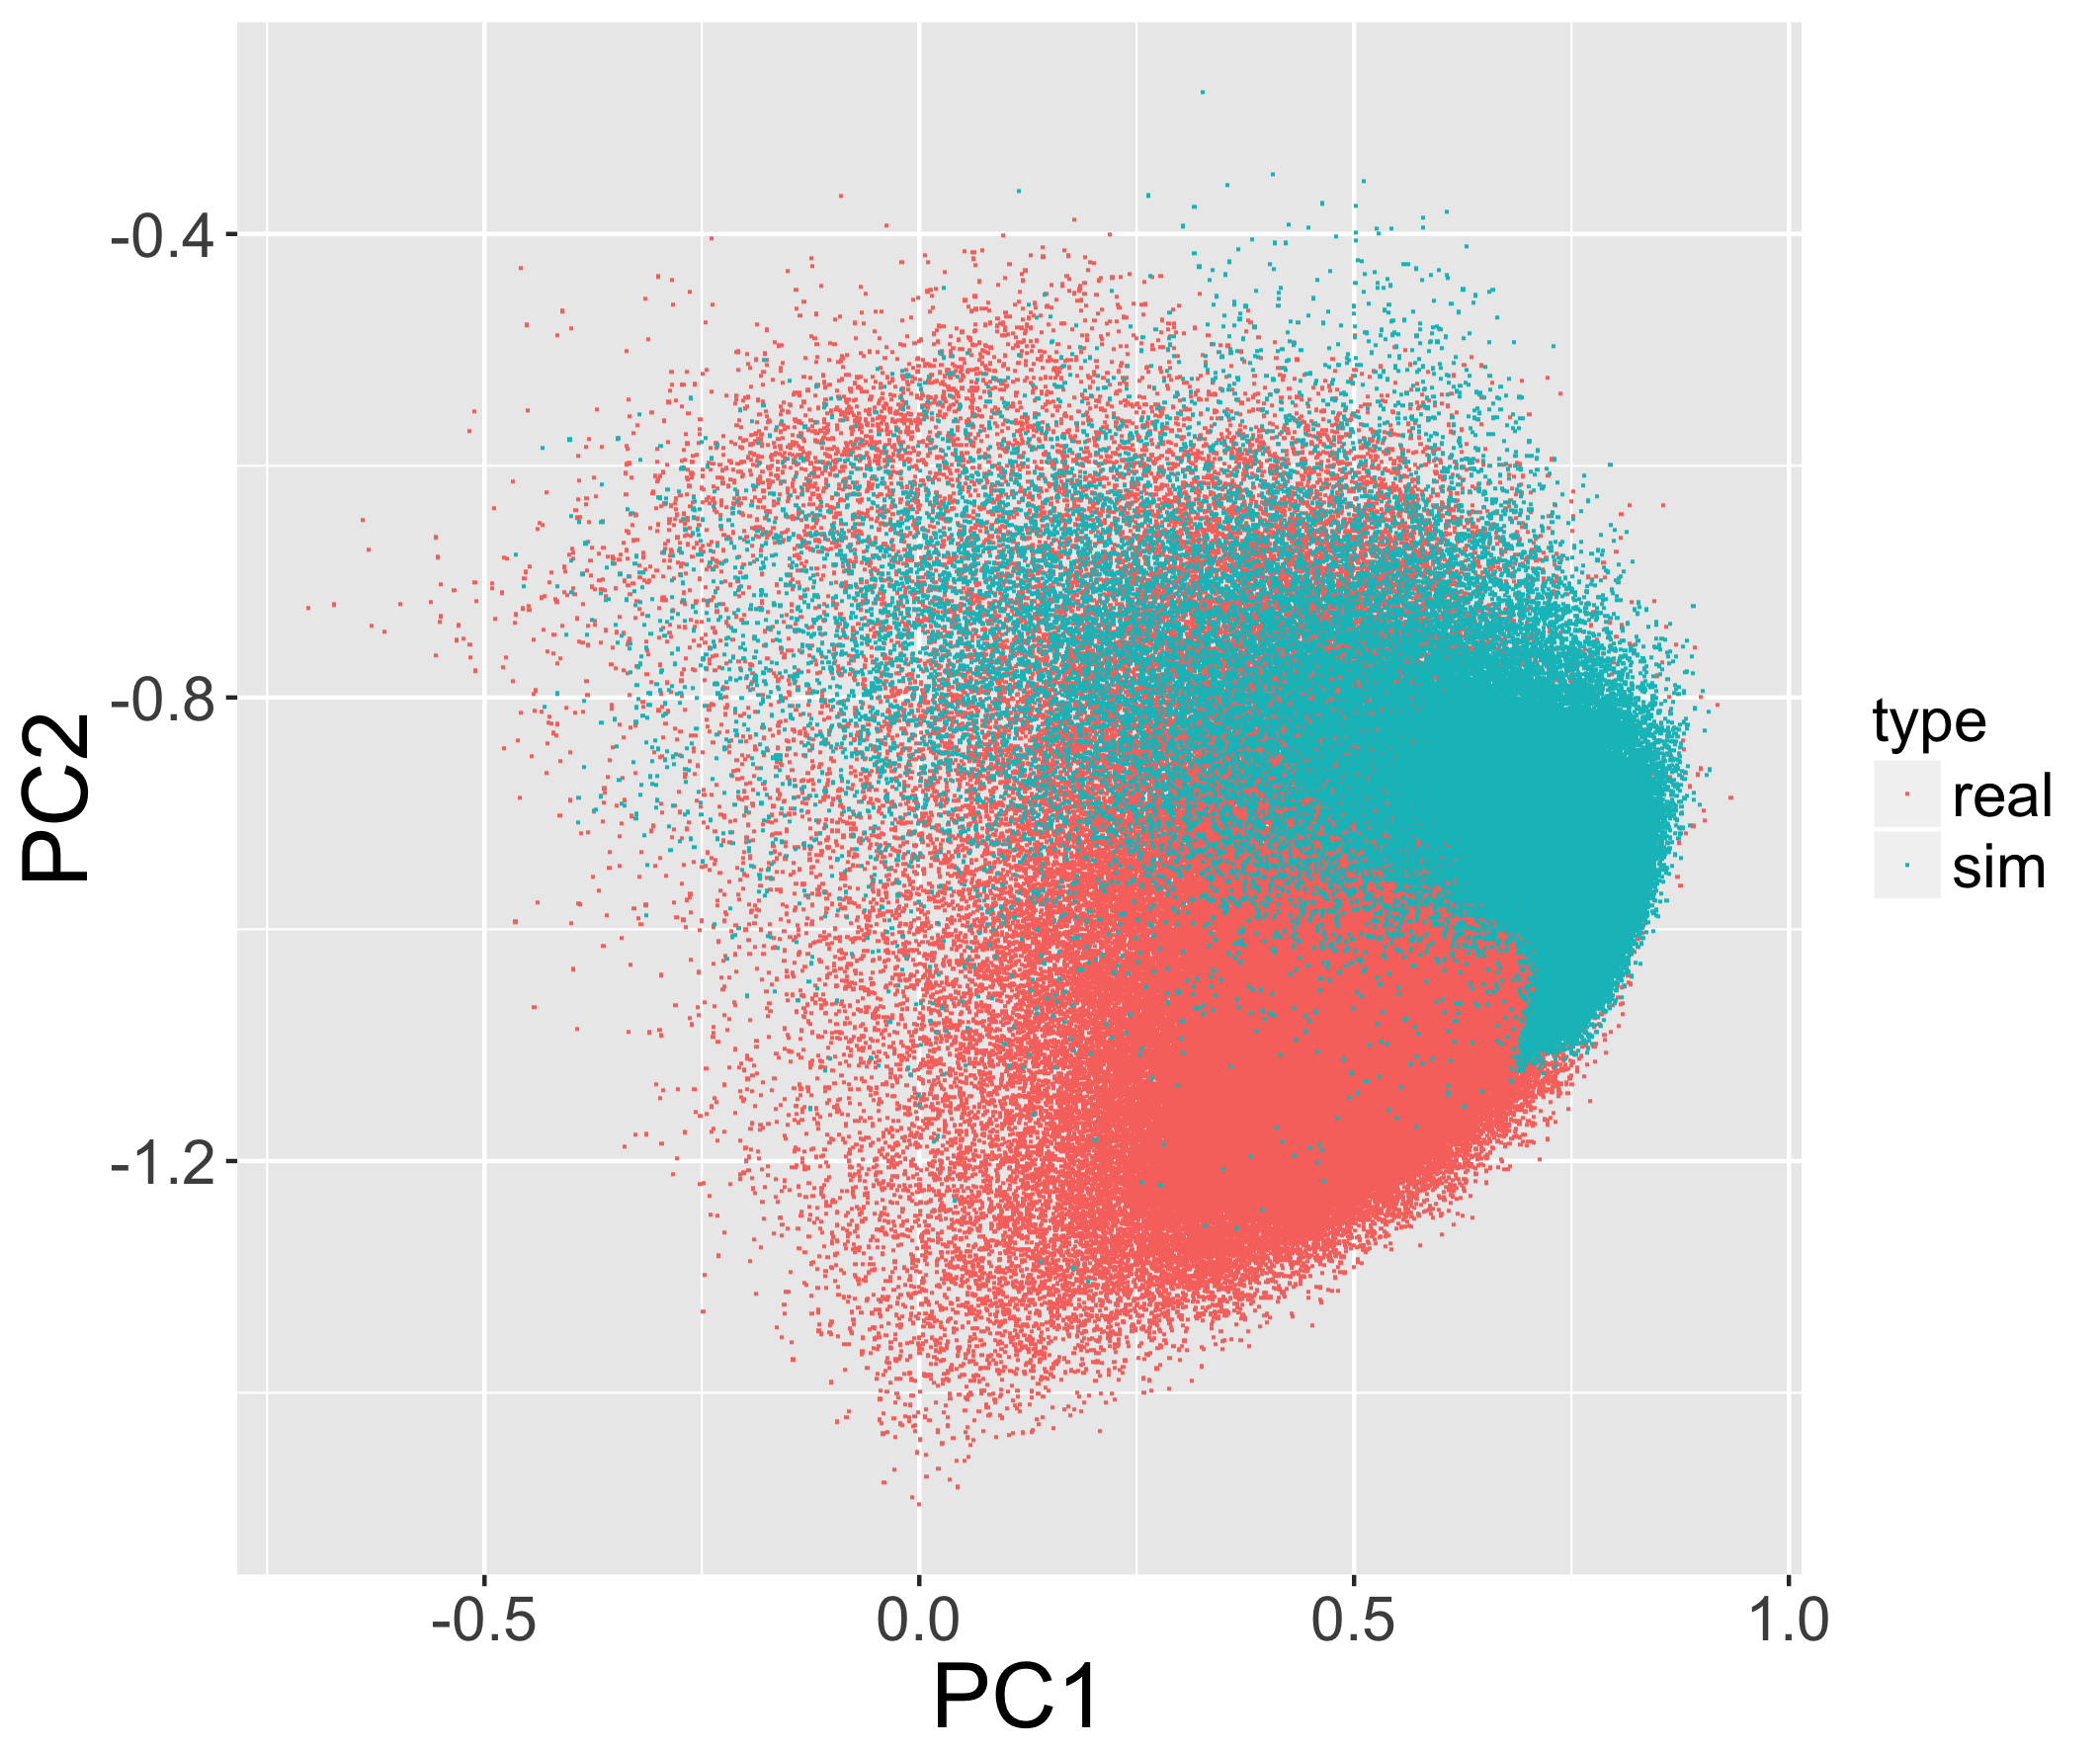
\includegraphics[width=\textwidth]{figures/coevol_pca_allobjs}
\column{0.2\textwidth}
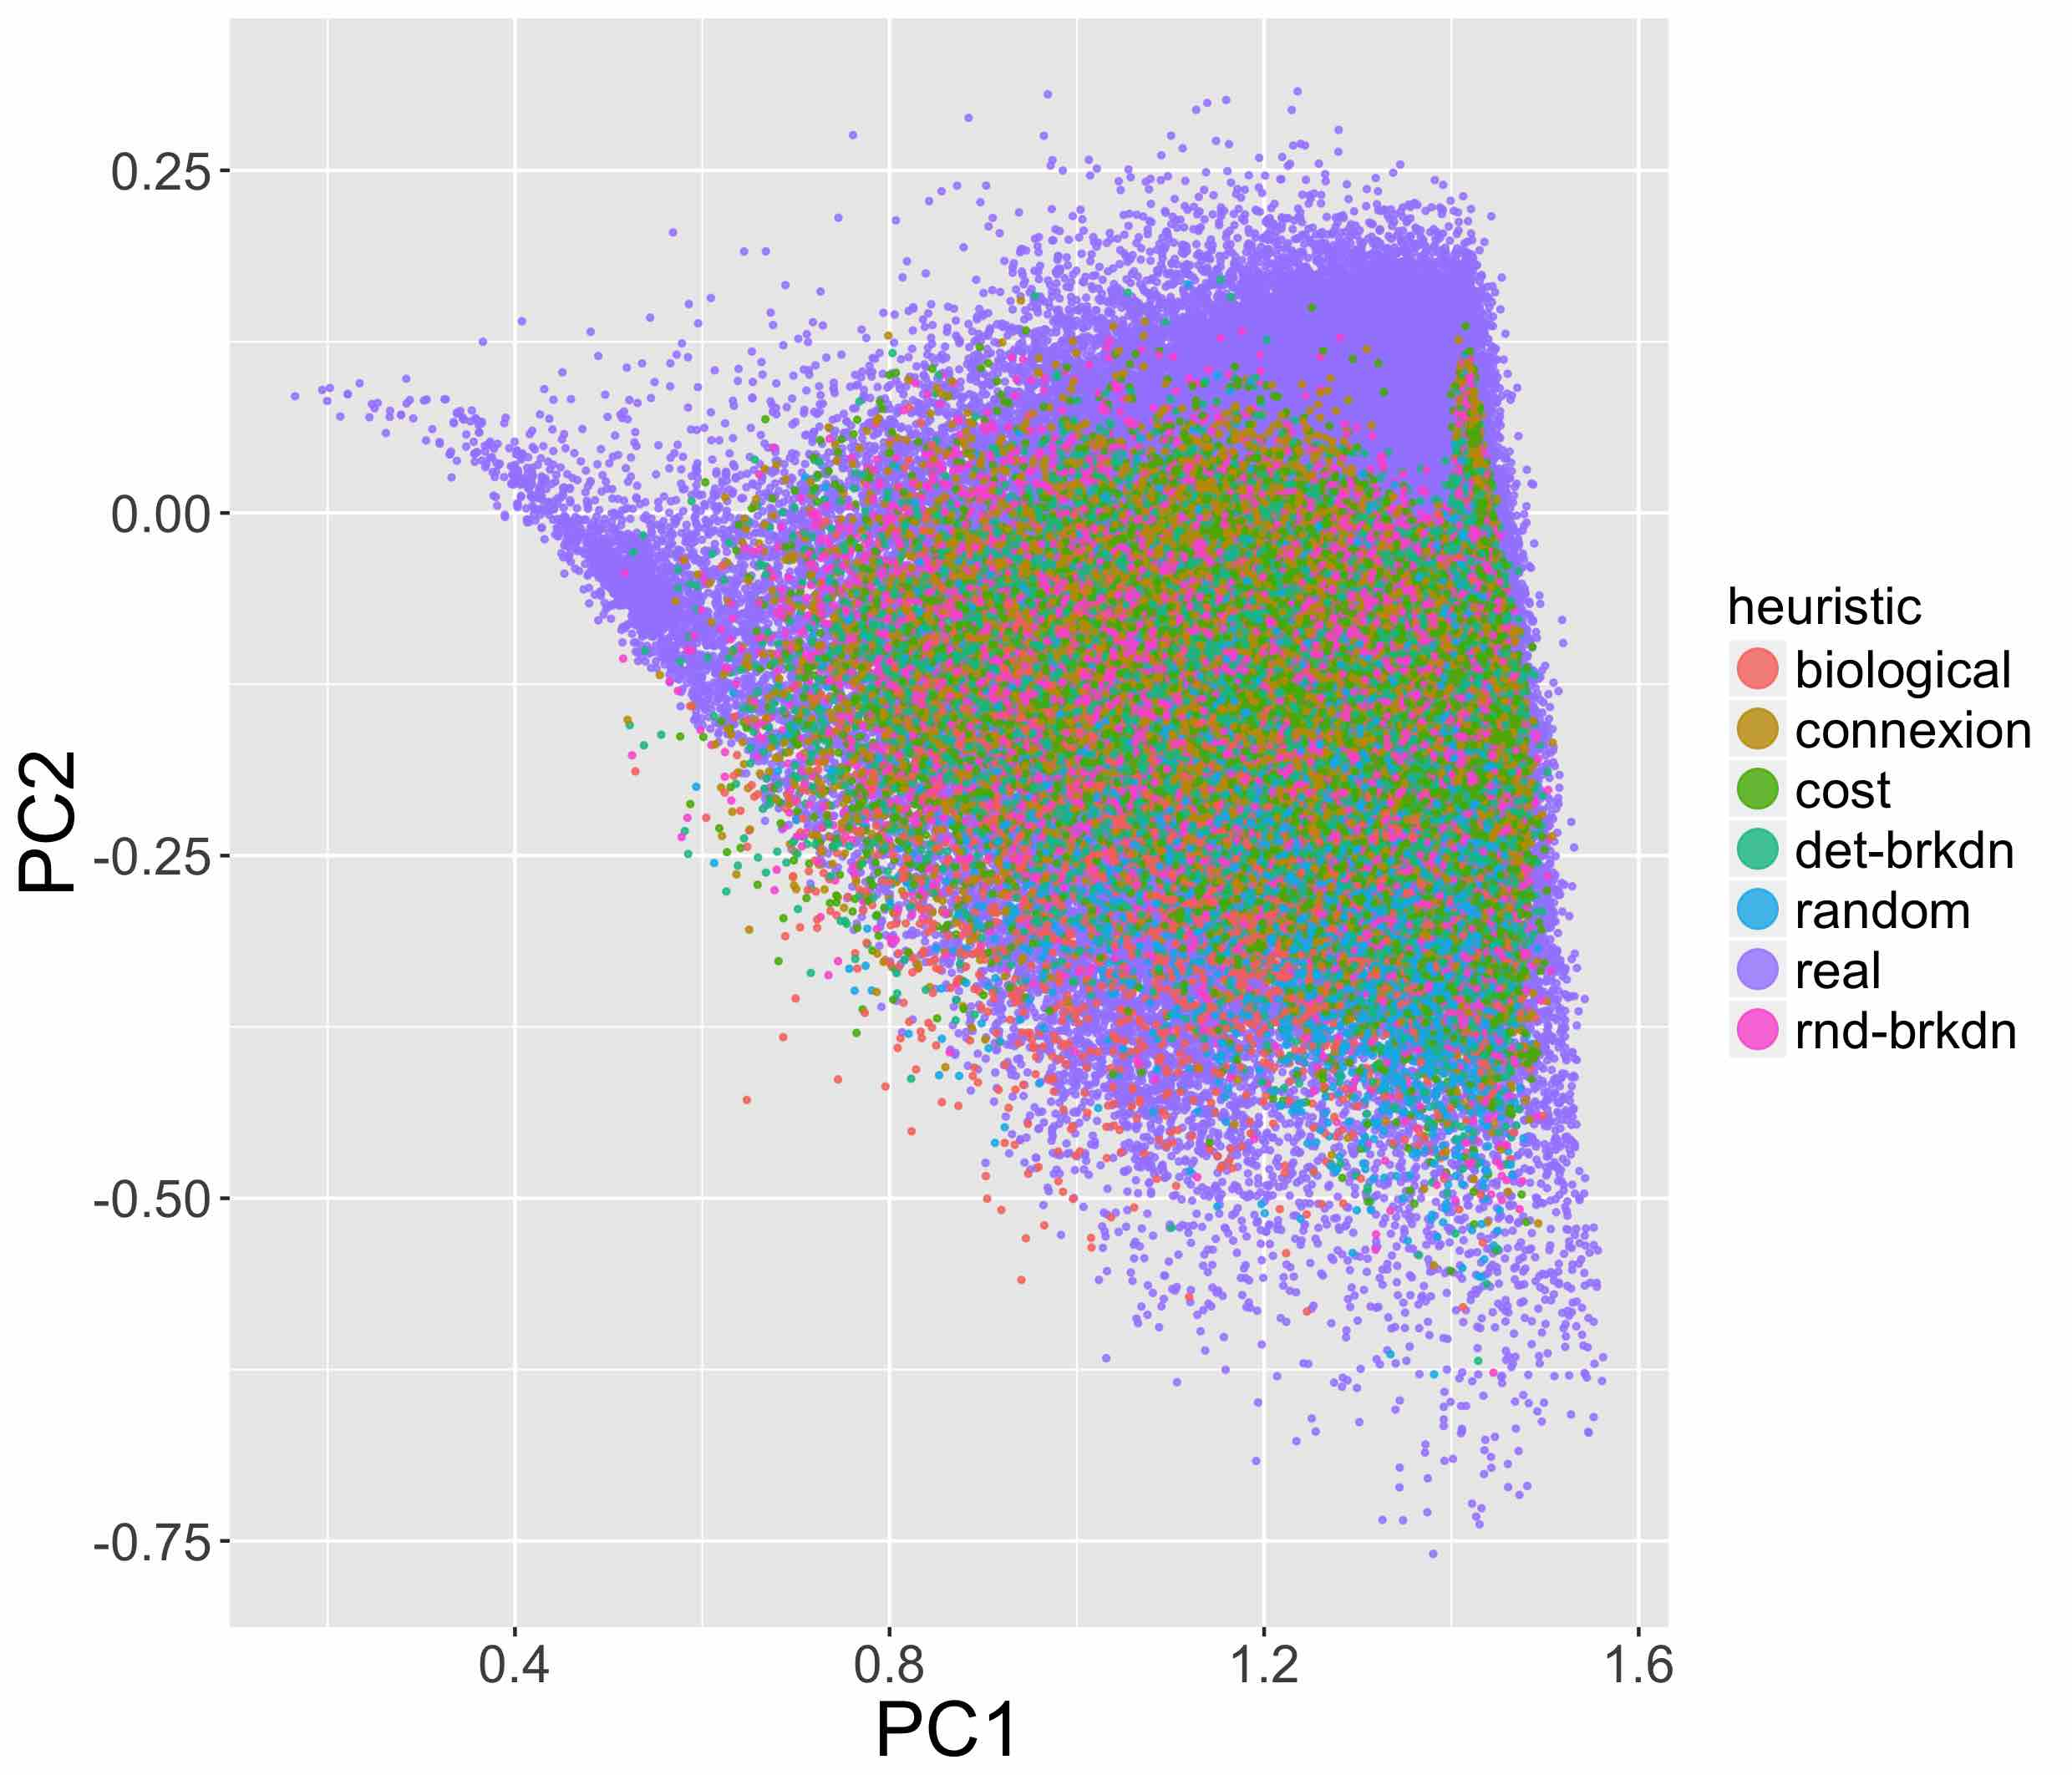
\includegraphics[width=\textwidth]{figures/coevol_pca_morpho_byheuristic}\\
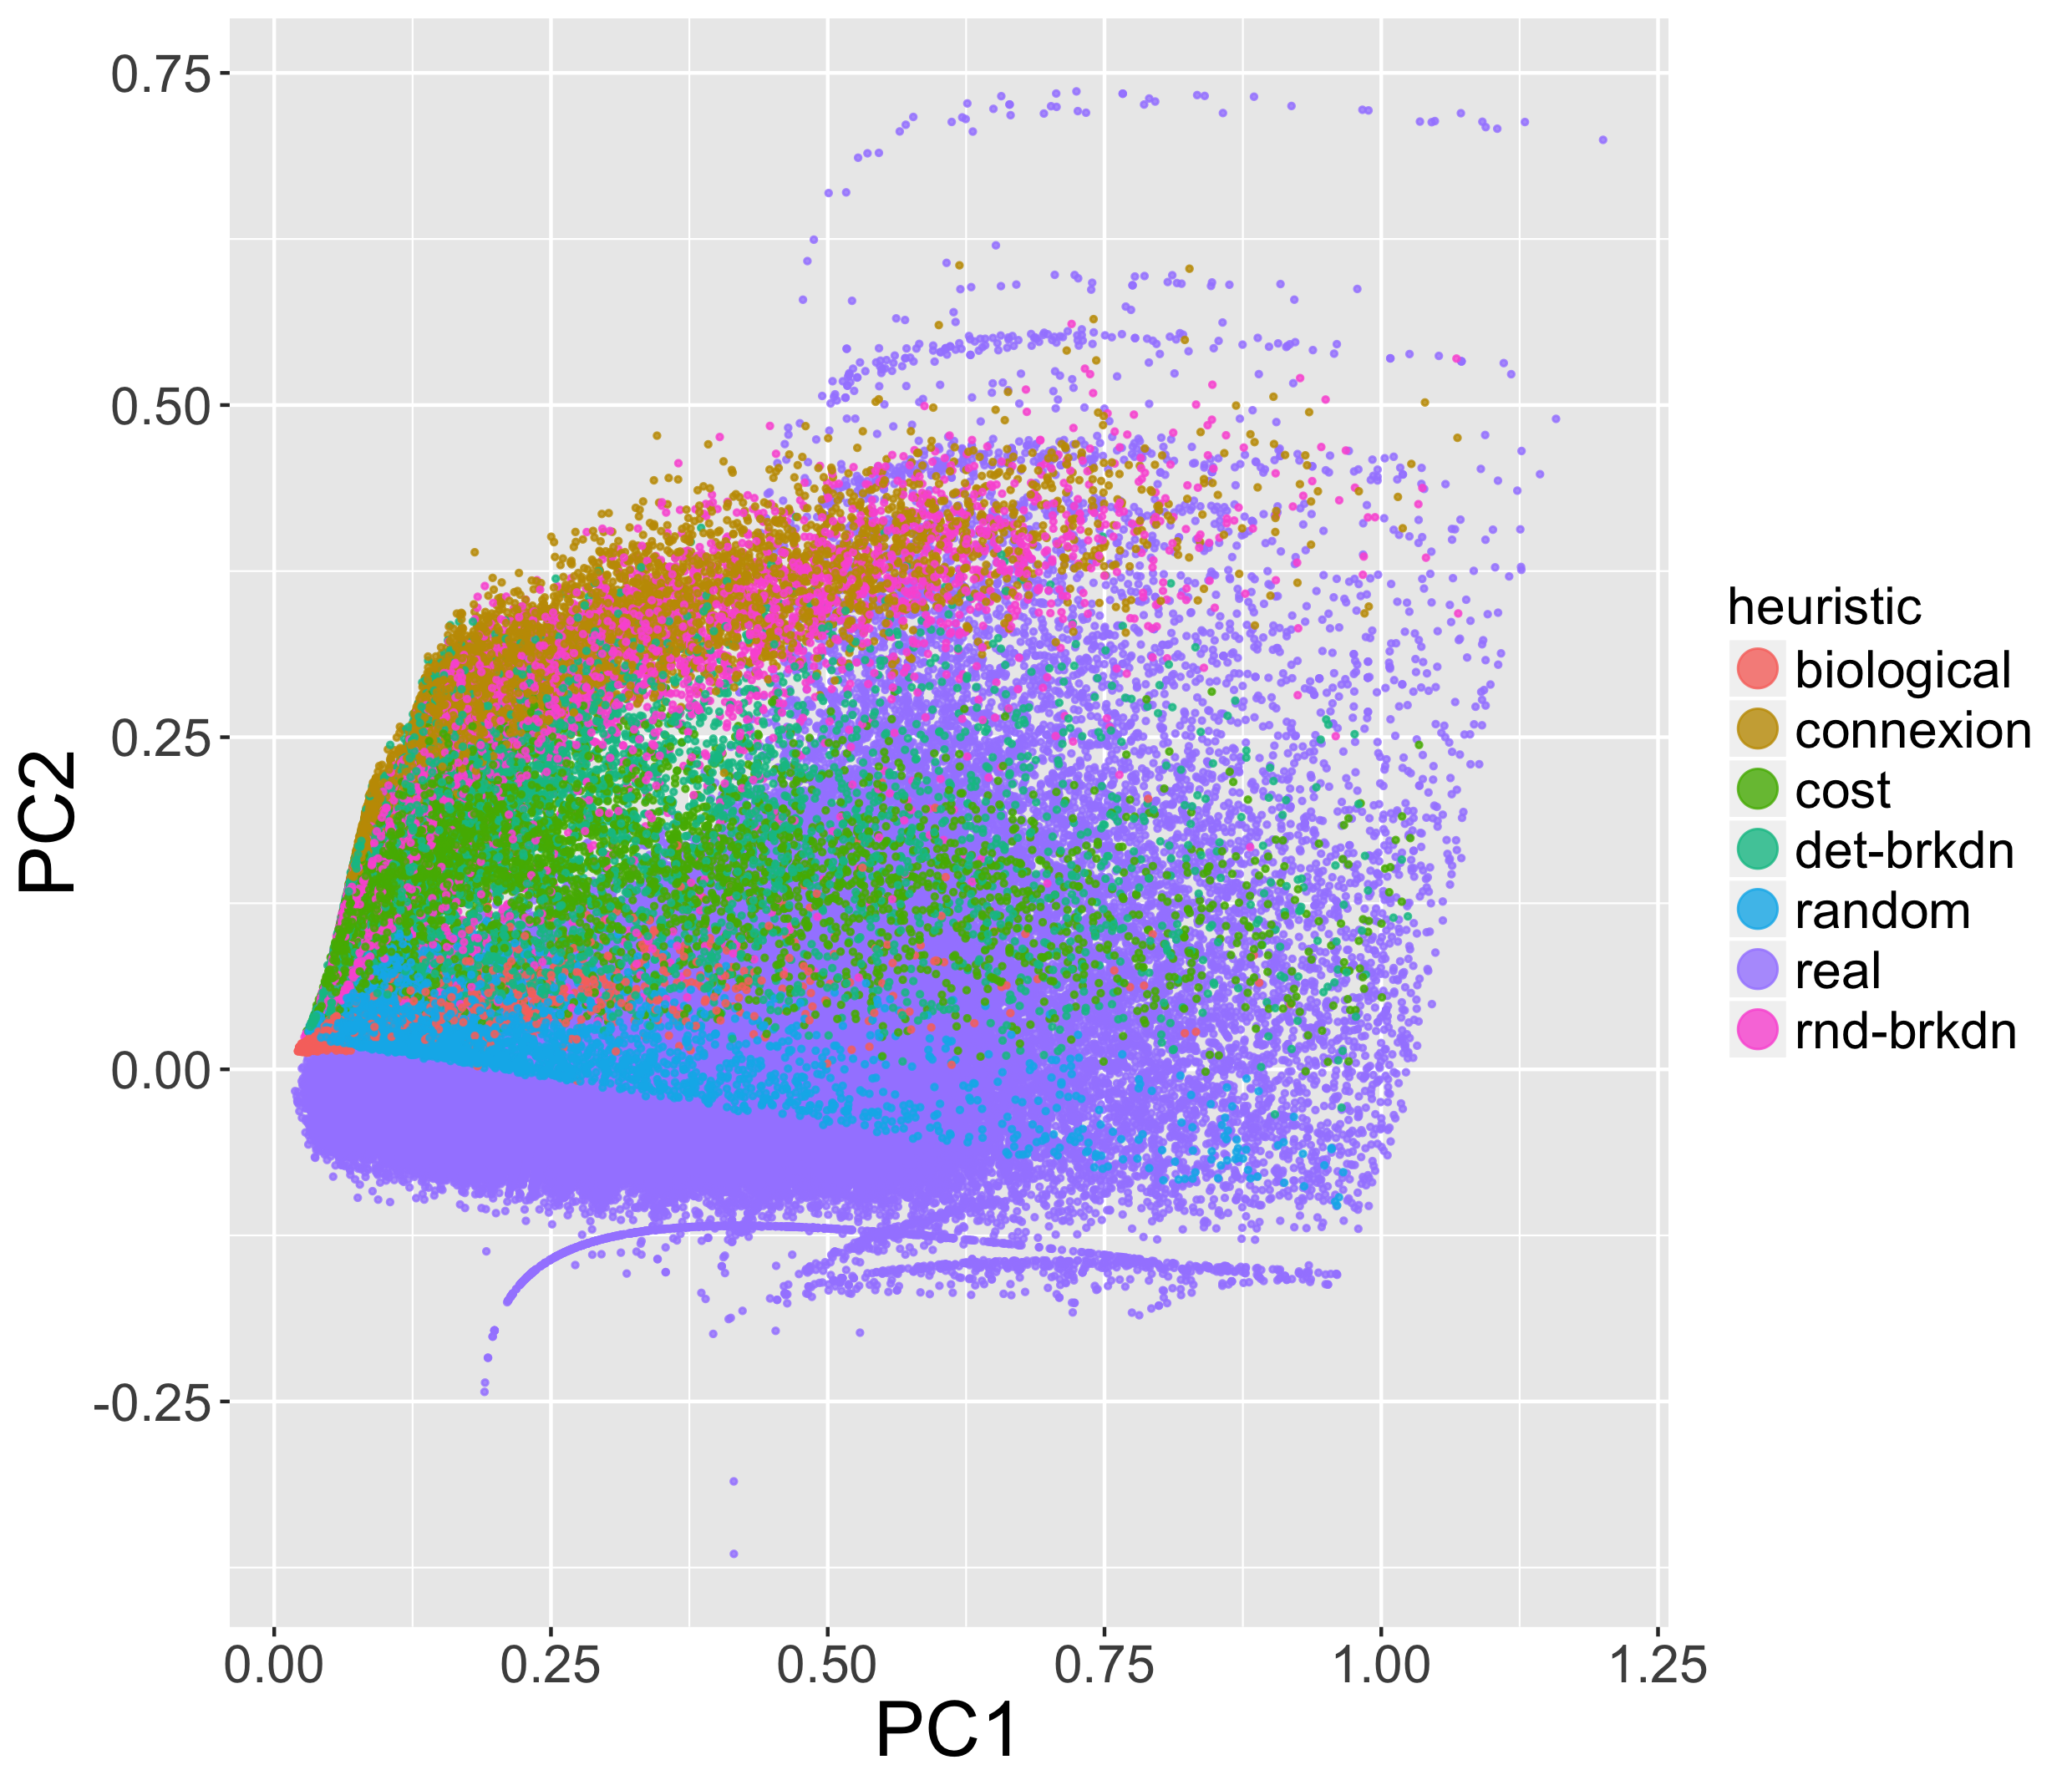
\includegraphics[width=\textwidth]{figures/coevol_pca_network_byheuristic}
\column{0.4\textwidth}
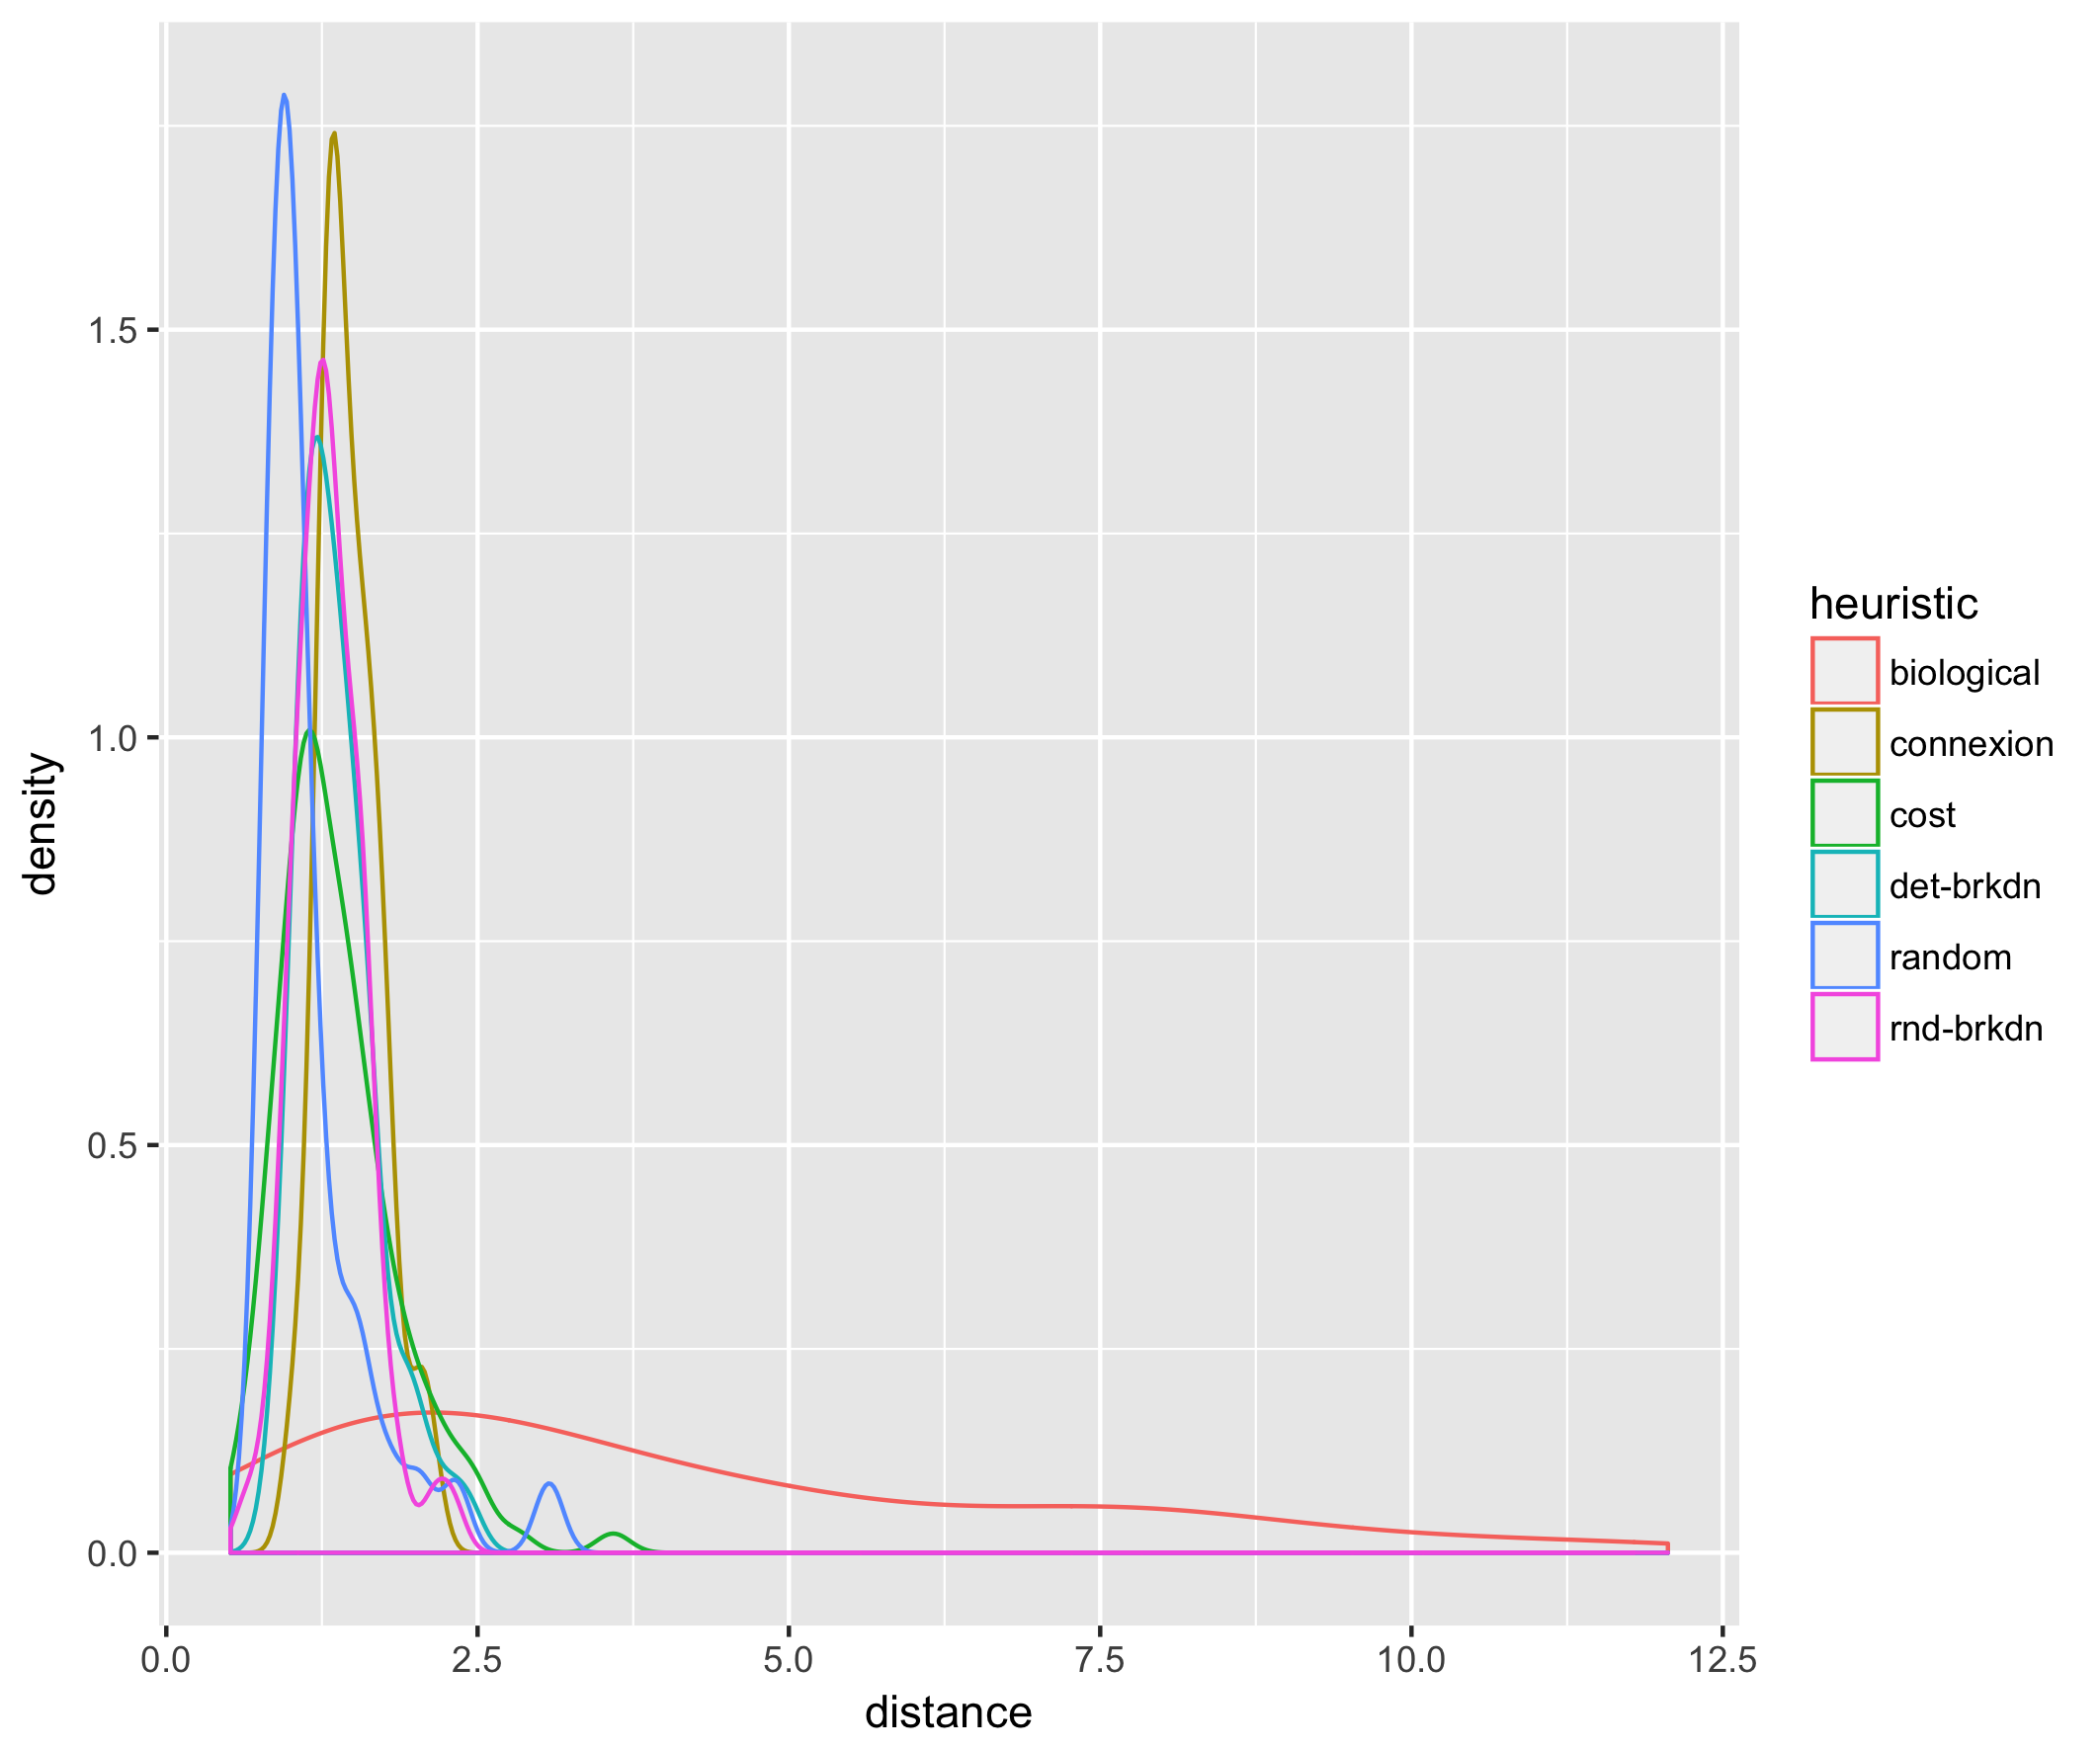
\includegraphics[width=\textwidth]{figures/coevol_corrs-distrib_rhoasize4}

\end{columns}

\footnotesize\textit{(Left) Full indicator space; (Middle) Morphological and Topology, by network heuristic; (Right) Distance distribution for cumulated distance for indicators and correlations.}

}


\sframe{Results : Causality Regimes}{

\textit{Unsupervised learning on lagged correlations between local variables unveils a diversity of causality regimes}

\medskip

\centering

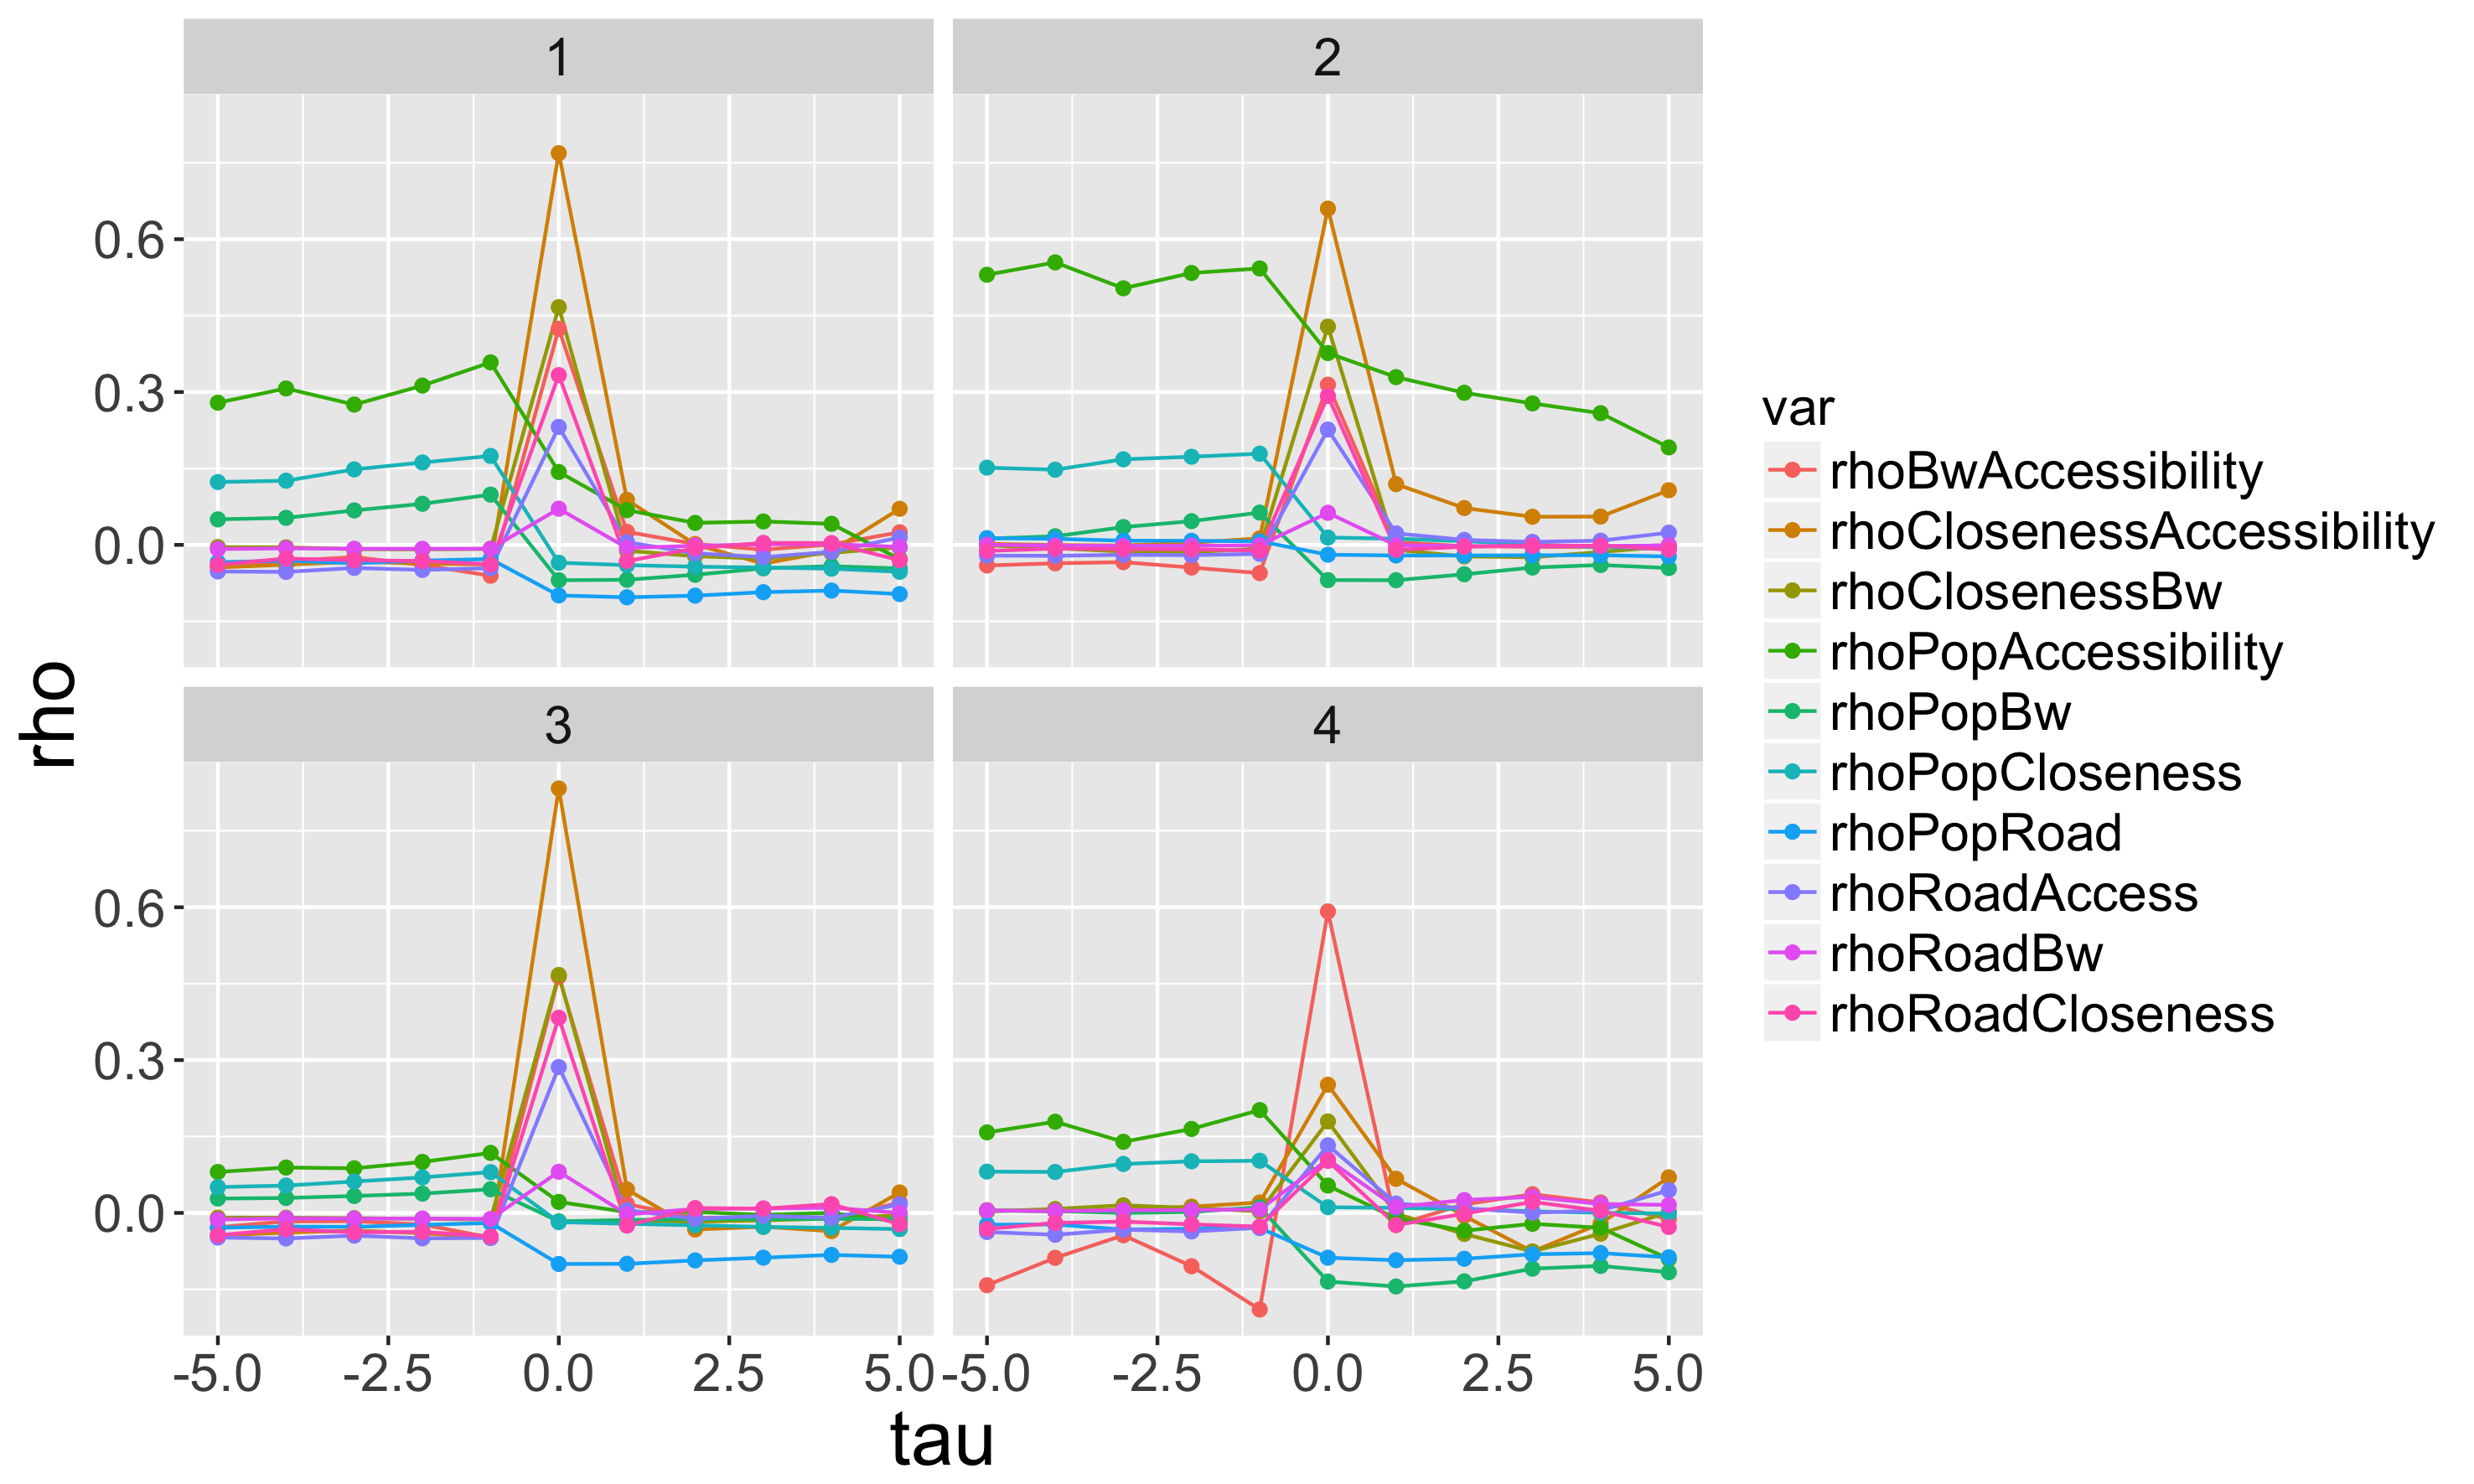
\includegraphics[width=0.52\textwidth,height=0.55\textheight]{figures/coevol_centertrajs}
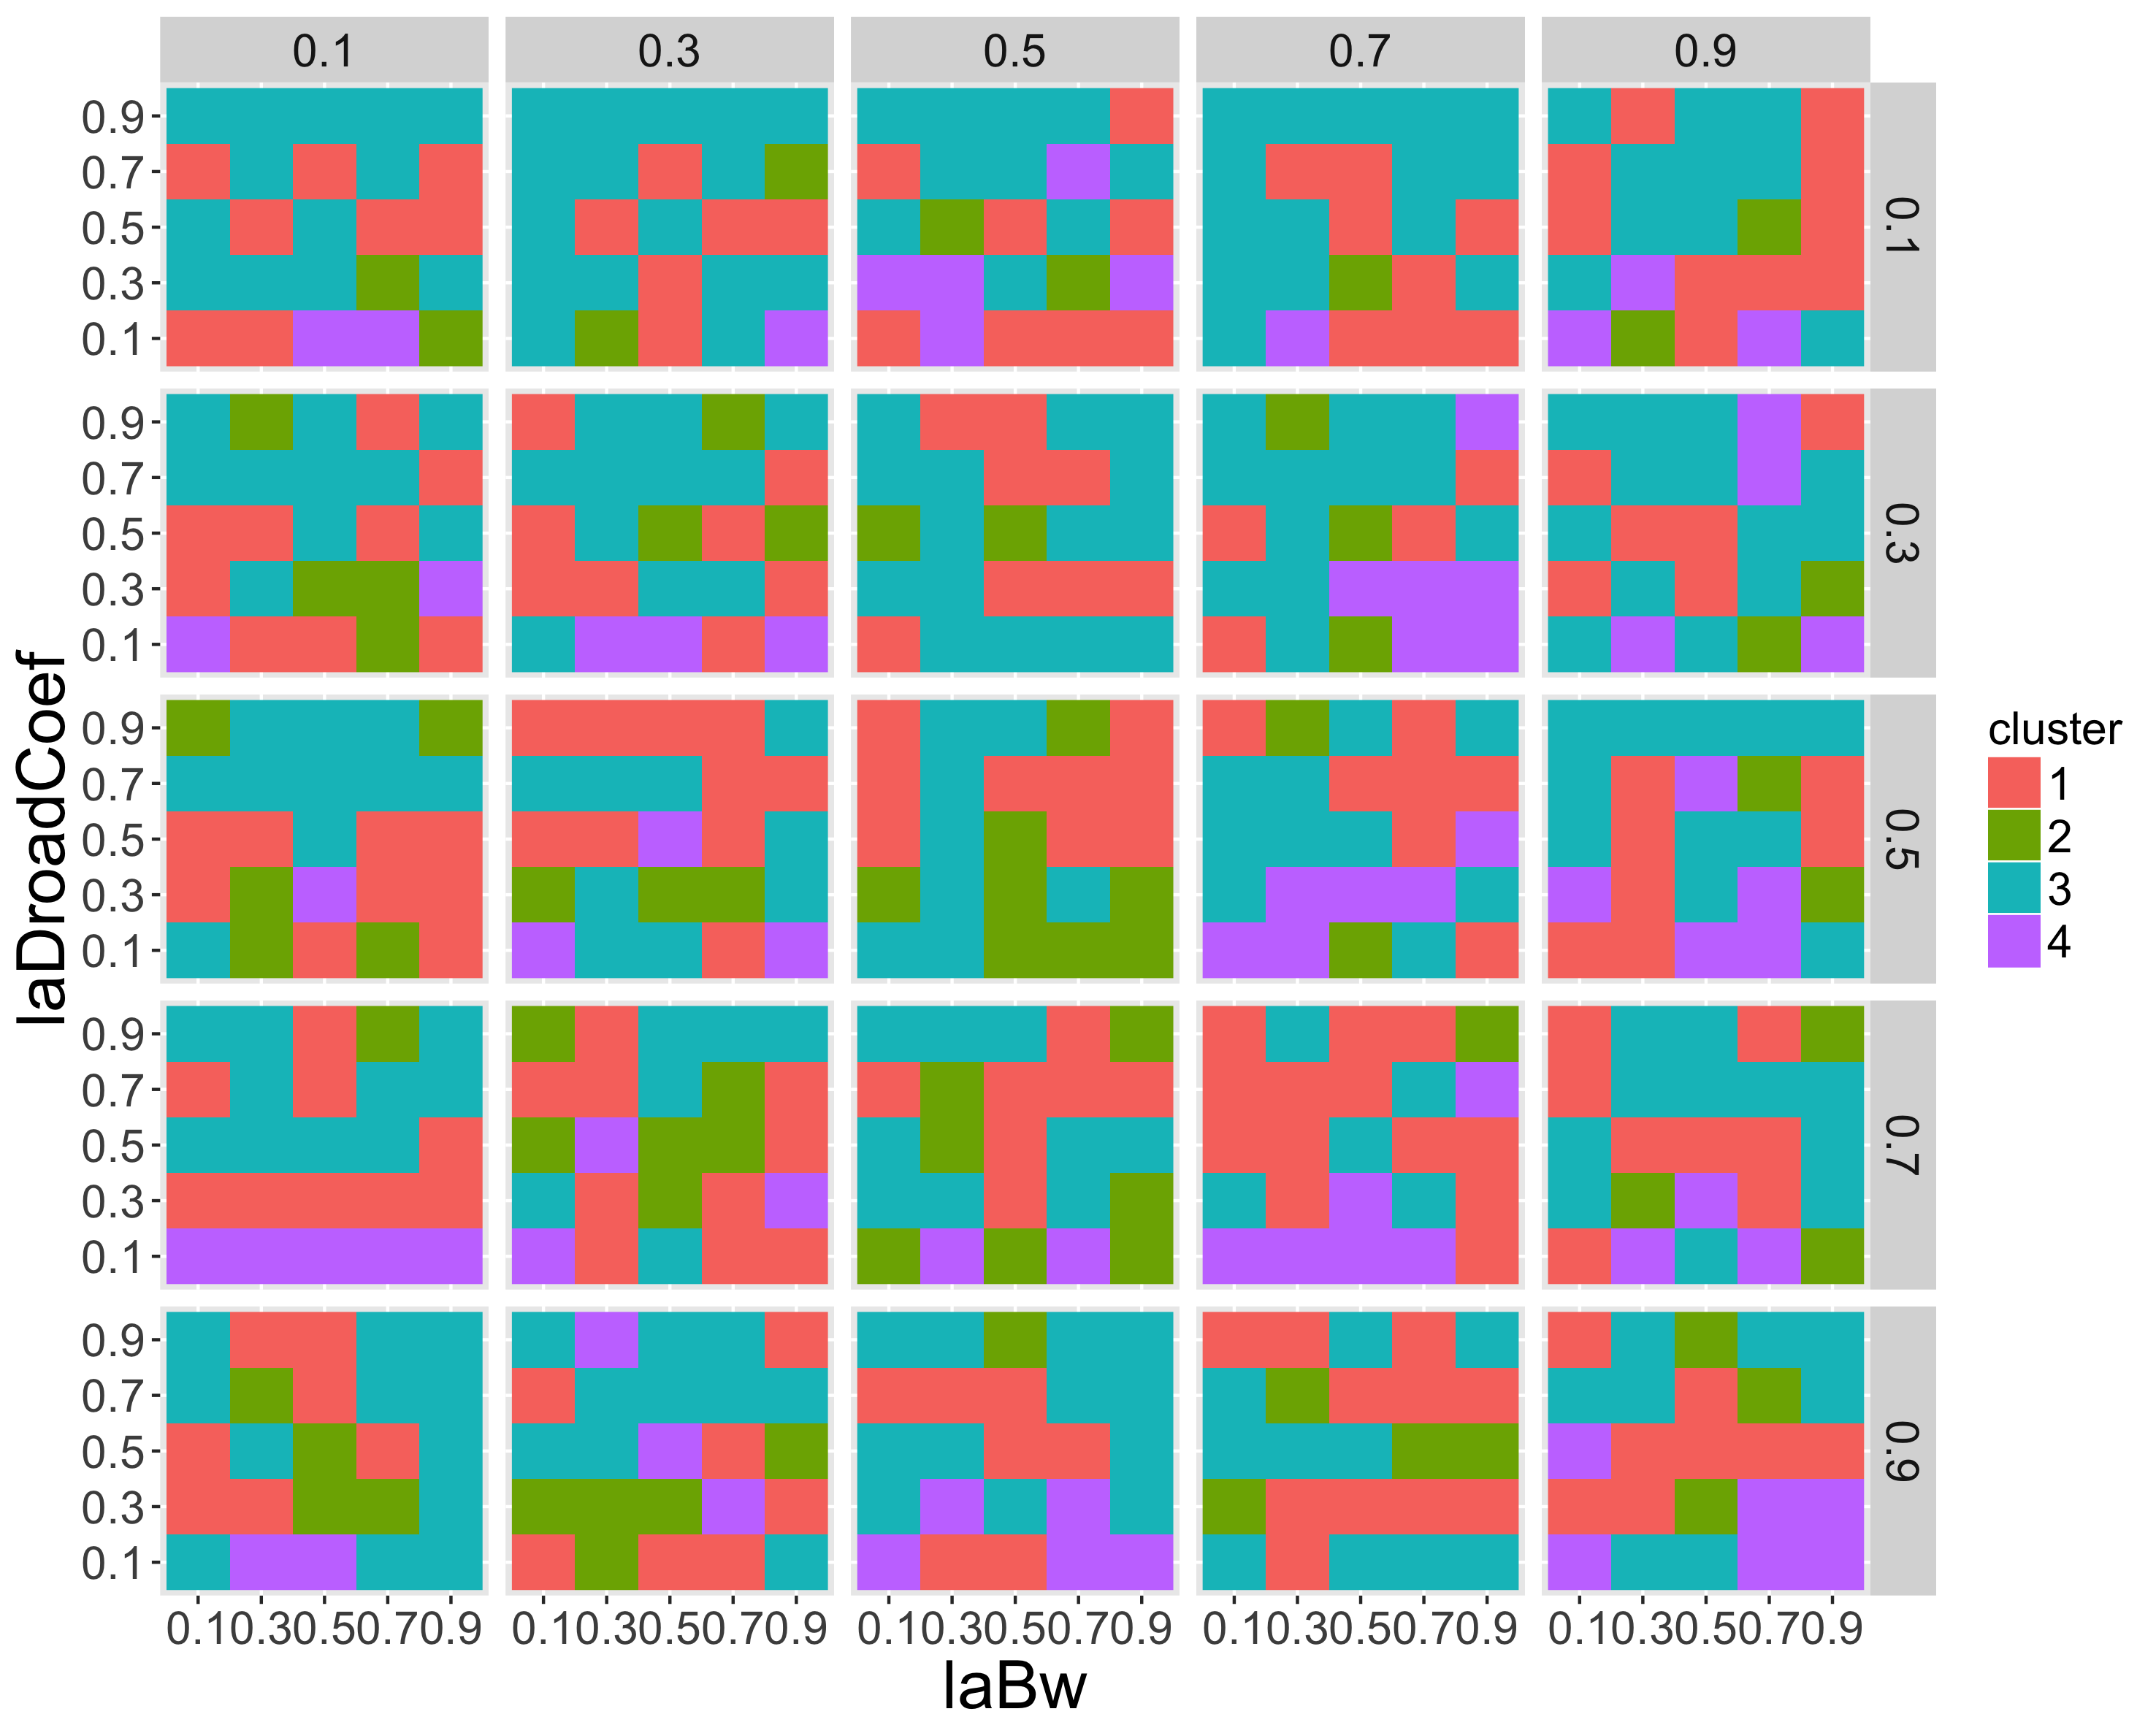
\includegraphics[width=0.4\textwidth,height=0.55\textheight]{figures/coevol_cluster-params}

\footnotesize\textit{(Left) Lagged correlation profiles of cluster centers; (Right) Distribution of regimes across parameter space}

}









\sframe{Reserve slides}{

\centering

\Large

\textbf{Reserve Slides}

}



%%%%%%%%%%%%%%%%%%%%%
\begin{frame}[allowframebreaks]
\frametitle{References}
\bibliographystyle{apalike}
\bibliography{/Users/juste/ComplexSystems/CityNetwork/Biblio/Bibtex/CityNetwork,biblio}
\end{frame}
%%%%%%%%%%%%%%%%%%%%%%%%%%%%





%
%
%
%
%\sframe{Modeling Urban Morphogenesis}{
%
%% Urban settlements and transportation networks are widely admitted to be co-evolving in the thematic and empirical studies of territorial systems. However, modeling approaches of such dynamical interactions between networks and territories are less developed. We propose to study this issue at an intermediate scale, focusing on morphological and functional properties of the territorial system in a stylized way.
%
%\justify
%
%\begin{columns}
%\column{0.35\textwidth}
%\centering
%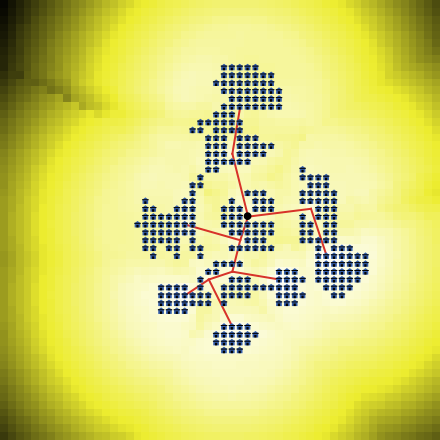
\includegraphics[width=\textwidth]{figures/RBD_lattice}\\
%\footnotesize\textit{Source: \cite{raimbault2014hybrid}}
%\column{0.62\textwidth}
%\justify
%\vspace{-1cm}
%\textbf{Morphogenesis :} \textit{Emergence of the form and the function in a strongly coupled manner, producing an emergent architecture~\cite{doursat2012morphogenetic}}
%\medskip
%
%$\rightarrow$ Co-evolution of Transportation Networks and Urban Settlements plays a specific role in real Urban Morphogenetic processes
%
%\end{columns}
%
%
%\bigskip
%
%\textbf{Research Objective : } Study a morphogenetic model at an intermediate scale, based on the co-evolution between a transportation network and population distribution.
%
%
%}
%
%
%
%

%
%
%
%
%
%
%\sframe{Discussion}{
%
%\justify
%
%\vspace{-1cm}
%
%\textbf{Implications}
%
%$\rightarrow$ This rather simple model reproduces most of existing urban forms in Europe for both population distribution and road network : which intrinsic dimension to the urban system and its morphological aspect ?
%
%$\rightarrow$ Ability to reproduce static correlations and a variety of dynamical lagged correlation regimes suggests that the model captures some of the processes of co-evolution
%
%\bigskip
%
%\textbf{Developments}
%
%% NOTE : not fair between heuristics, not same number of params - but open question.
%
%% NOTE : indicators not sufficient to capture full nw topology ?
%
%% - check best processes for a particular given configuration.
%
%$\rightarrow$ Towards a dynamical calibration, despite the sparsity of dynamical data
%
%$\rightarrow$ Investigate the link between spatial non-stationarity and non-ergodicity through simulation by the model
%
%$\rightarrow$ Compare network in a ``fair'' way (correcting for additional parameters, open question for models of simulation)
%
%}
%
%
%
%
%\sframe{Conclusion}{
%
%\justify
%
%$\rightarrow$ A novel model of urban morphogenesis at the mesoscopic scale systematically explored : need for more coupling and comparison of models.
%
%\medskip
%
%$\rightarrow$ At the macro scale of the system of cities ? Need for multi-scale models.
%
%\medskip
%
%$\rightarrow$ With more refined urban characteristics and other dimensions ? Need for more interdisciplinarity.
%
%\bigskip
%\bigskip
%\bigskip
%
%\footnotesize{ - Code, data and results available at\\ \texttt{https://github.com/JusteRaimbault/CityNetwork}
%
%}
%
%}
%
%
%
%
%
%\sframe{Defining co-evolution}{
%
%
%\justify
%
%No clear definition of co-evolution in the literature : \cite{bretagnolle:tel-00459720} distinguishes ``reciprocal adaptation'' where a sense of causality can clearly be identified, from co-evolutive regimes 
%
%
%\bigskip
%\bigskip
%
%\cite{raimbault2017identification} identifies multiple causality regimes in a simple strongly coupled growth model $\rightarrow$ to be put in perspective with a theoretical definition of co-evolution based on the conjunction of Morphogenesis and the Evolutive Urban Theory, summarised by~\cite{raimbault2017co}
%
%}
%
%\sframe{Modeling Urban Morphogenesis and Co-evolution}{
%
%\justify
%
%\textbf{Morphogenesis :} \cite{makse1998modeling} correlated growth; 
%
%\cite{10.1371/journal.pone.0133780} multi-scale migration and percolation; 
%
%\cite{bonin2012modele} qualitative differentiation of urban function; 
%
%\cite{achibet2014model} procedural model at the micro-scale 
%
%\bigskip
%
%\textbf{Co-evolution :} \cite{baptistemodeling} system dynamics with evolving capacities; \cite{wu2017city} population diffusion and network growth; 
%
%\cite{blumenfeld2010network} and \cite{schmitt2014modelisation} : random potential breakdown for network growth.
%
%}
%
%
%\sframe{Real Data : indicators}{
%
%\centering
%
%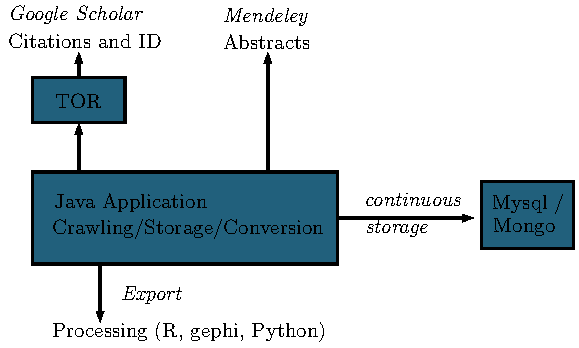
\includegraphics[width=0.45\textwidth]{figures/Fig1}\hspace{0.1cm}
%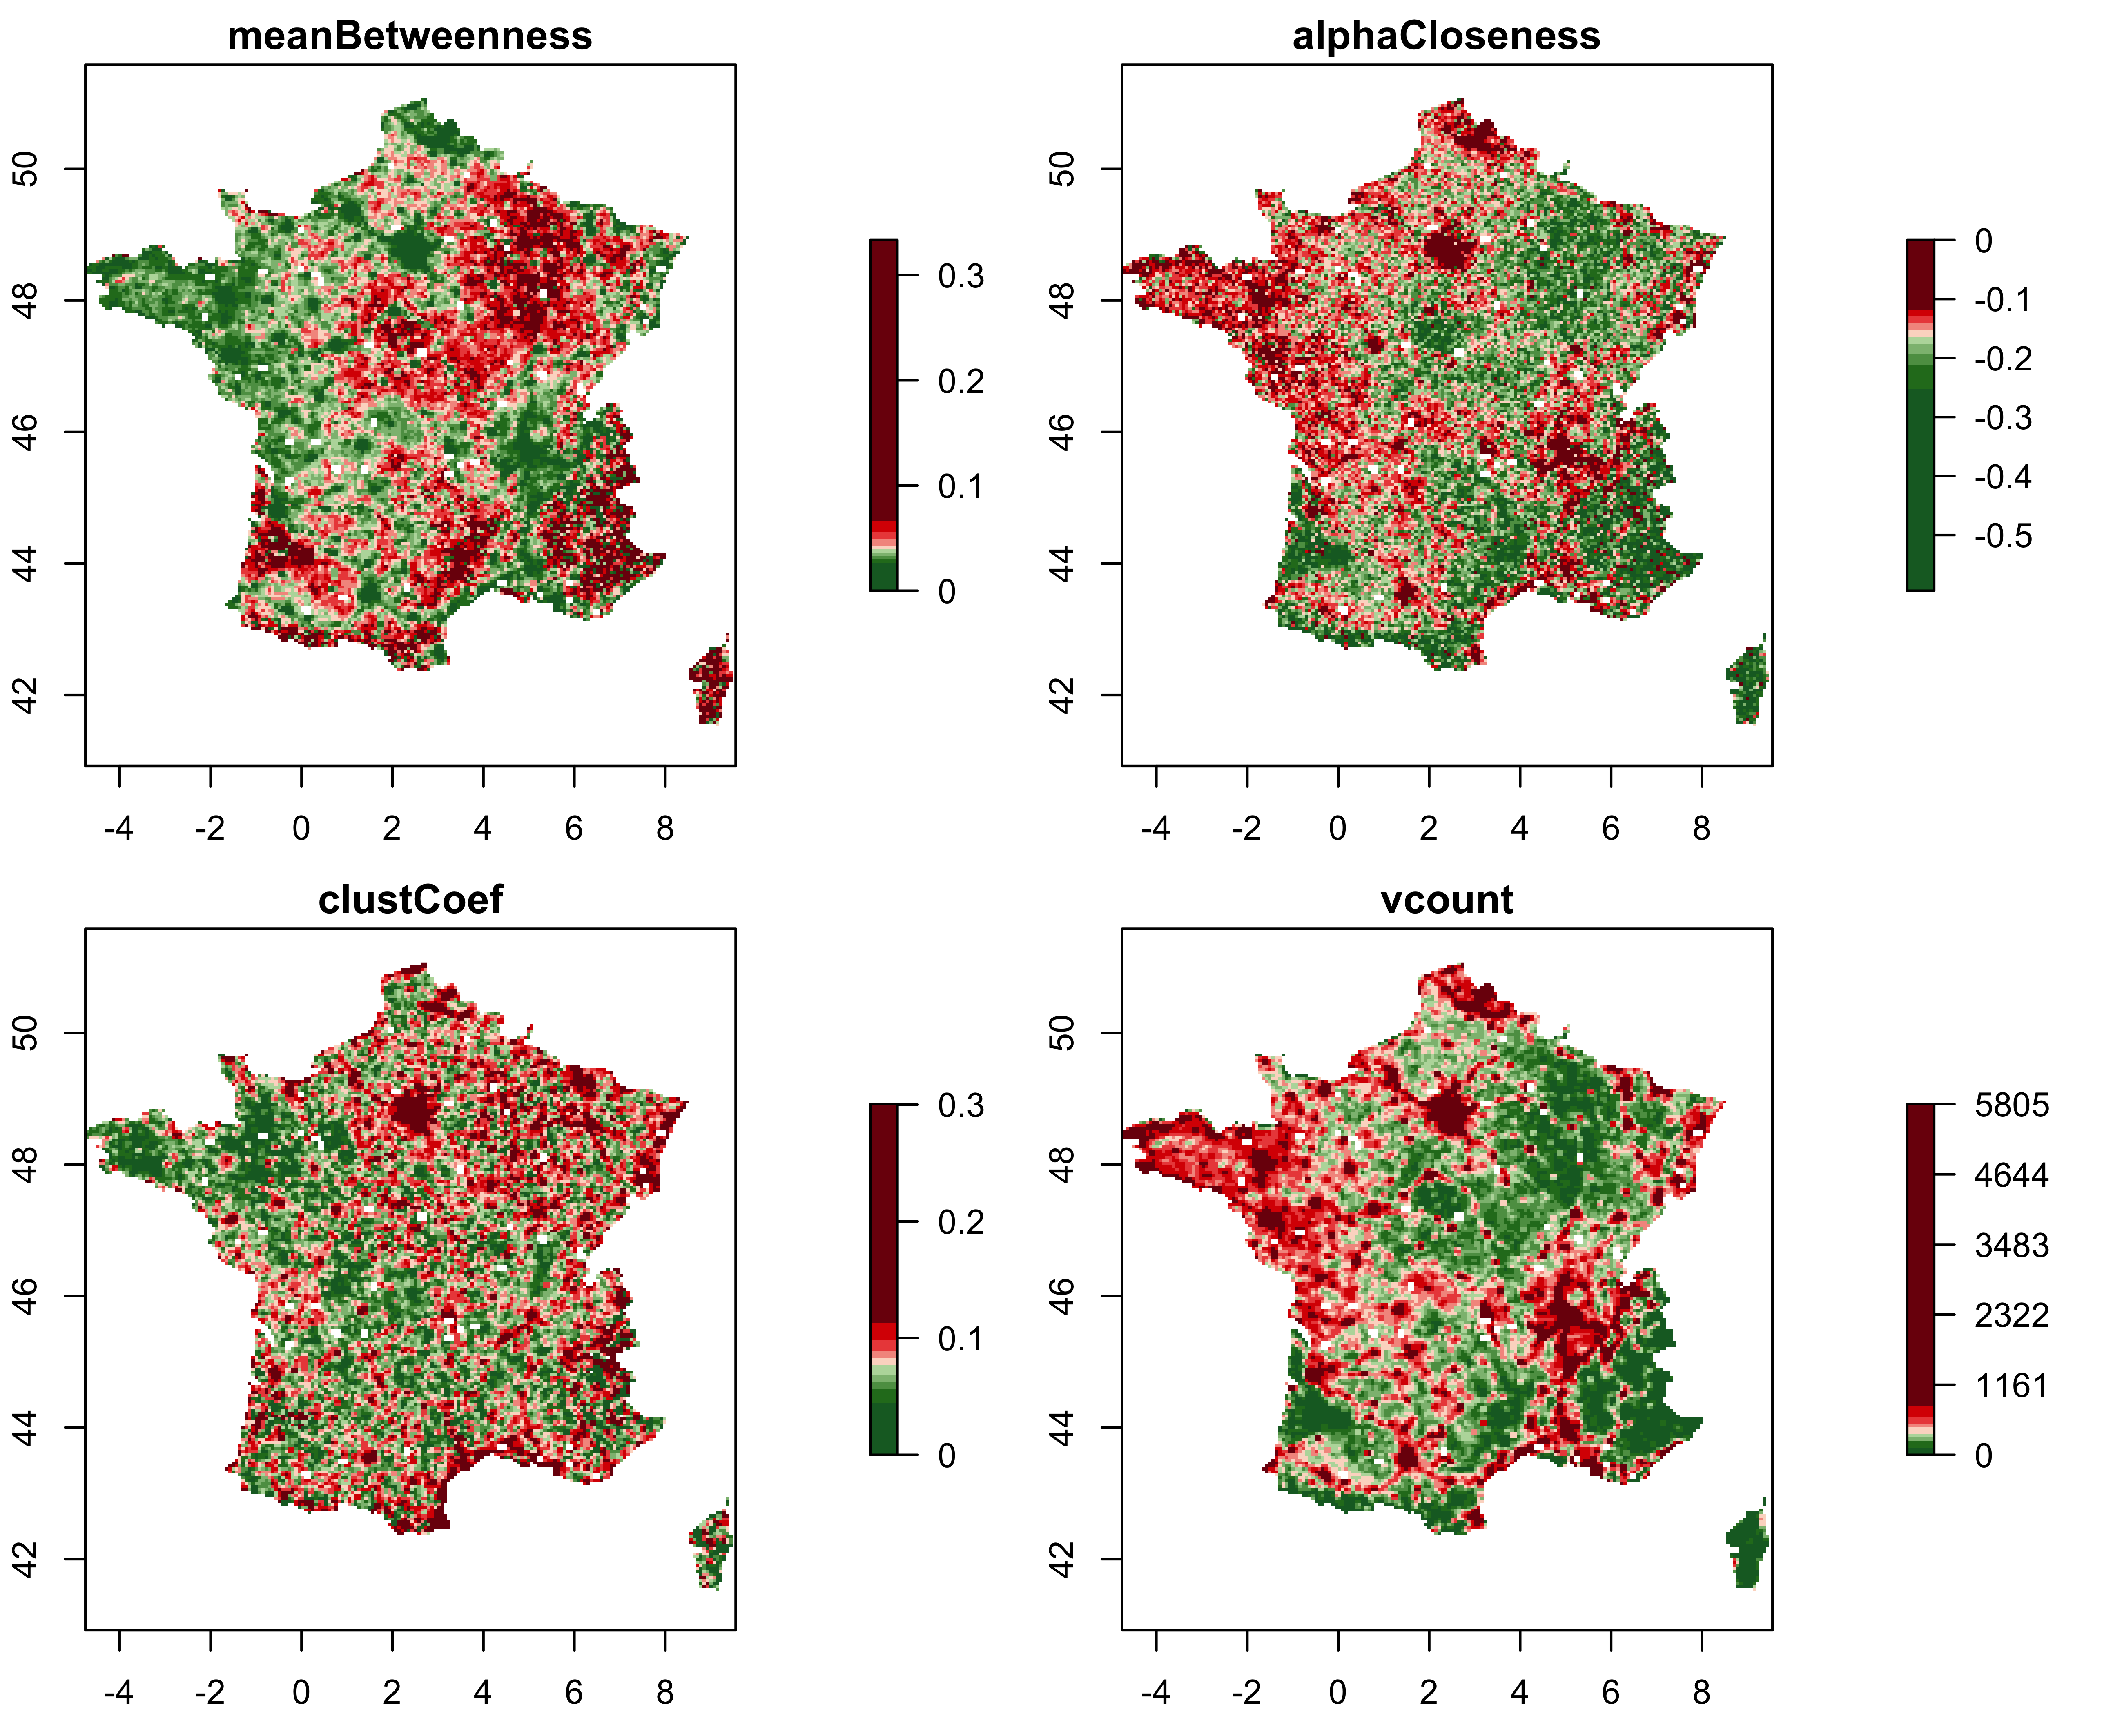
\includegraphics[width=0.53\textwidth]{figures/FR_indics_network_selected_2_discrquantiles}
%
%}
%
%\sframe{Real Data : correlations}{
%
%\centering
%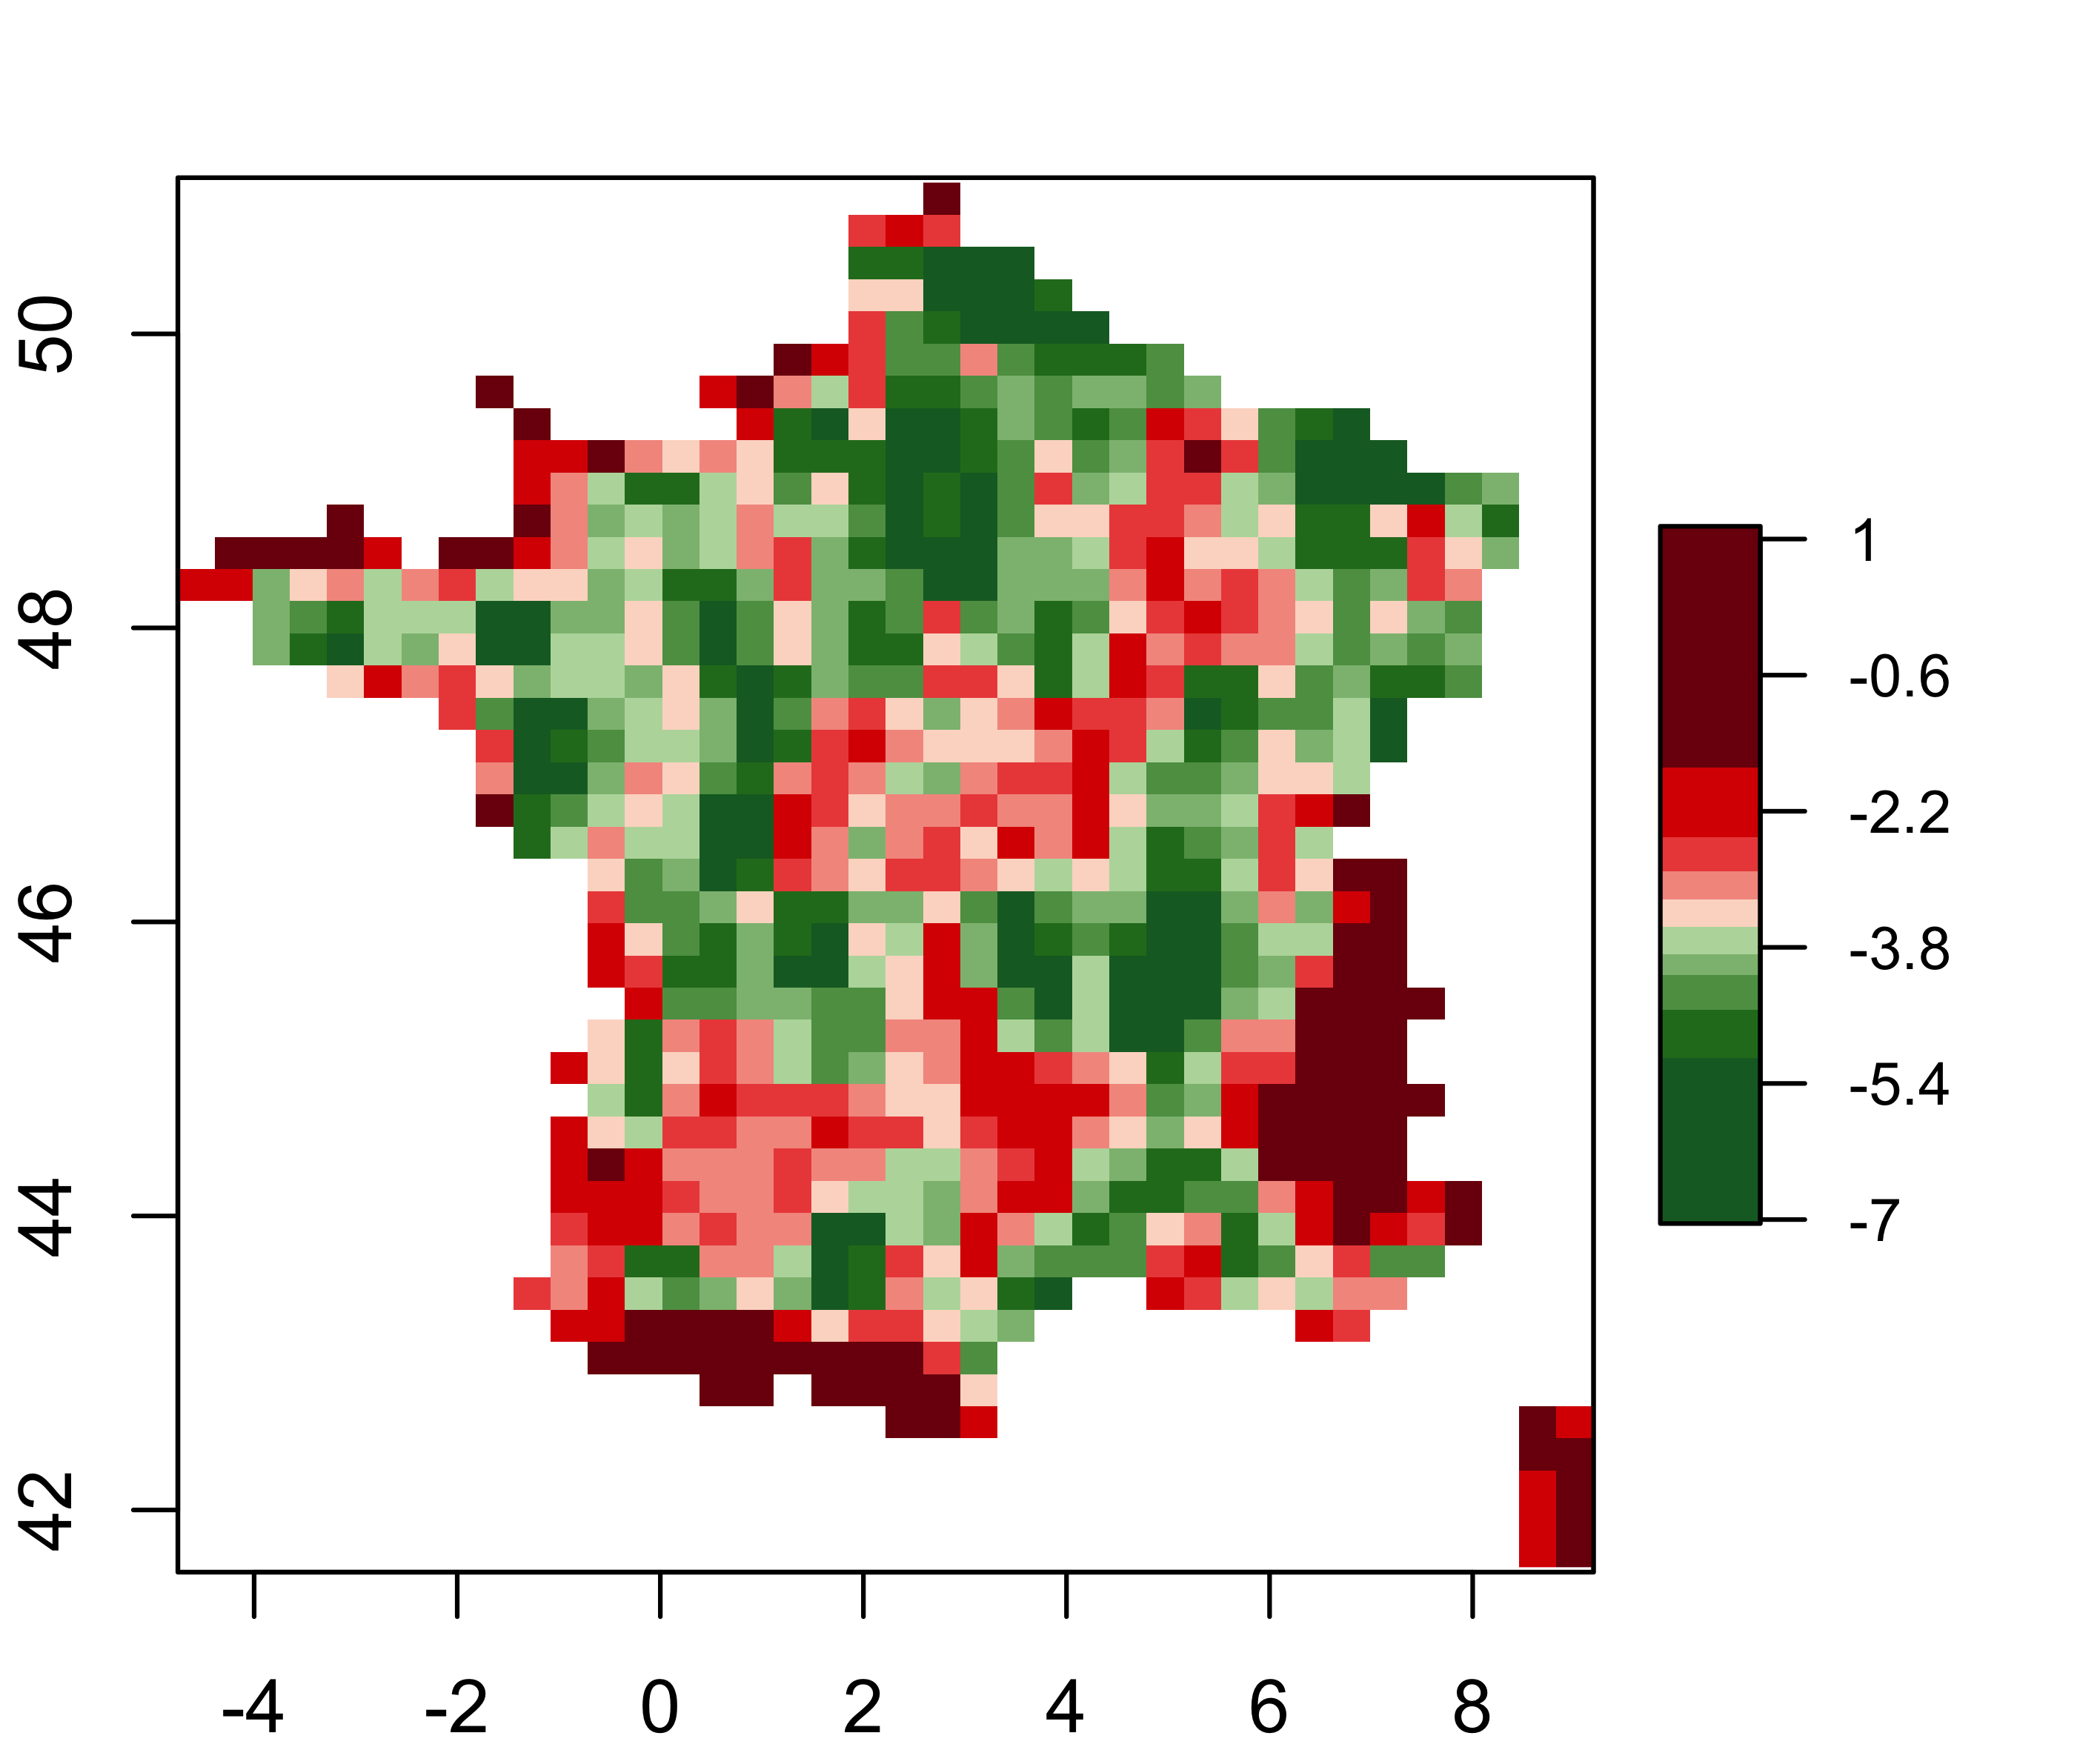
\includegraphics[width=0.7\textwidth]{figures/FR_corr_PCA_rhoasize12}
%
%}
%
%\sframe{Indicators}{
%
%Urban morphology measured by:
%
%\begin{itemize}
%	\item Spatial autocorrelation (Moran Index)
%	\item Average distance
%	\item Entropy
%	\item Hierarchy (OLS slope for rank-size)
%\end{itemize}
%
%\medskip
%
%Network Topology measured by:
%
%\begin{itemize}
%	\item Betweenness and Closeness centralities: average and hierarchy
%	\item Accessibility (weighted closeness)
%	\item Efficiency (network pace relative to euclidian distance)
%	\item Mean path length, diameter
%\end{itemize}
%
%}
%
%
%
%
%\sframe{Model specification}{
%
%\footnotesize
%
%Patch utility given by $U_i = \sum_k w_k \cdot \tilde{x}_k$ with $\tilde{x}_k$ normalized local variables among population, betweenness and closeness centrality, distance to roads, accessibility ; aggregation done with probability $\left(U_i/\sum_k U_k\right)^\alpha$ ; diffusion among neighbors $n_d$ times with strength $\beta$
%
%\medskip
%
%\textbf{Network Generation :}
%
%Adding a fixed number $n_N$ of new nodes : for patches such that $d_r < d_0$, probability to receive a node is
%
%% note : not a proba for the last ? no pb as soon as in 0,1, realized anyway.
%\[
%p = P/P_{max} \cdot (d_M - d)/d_M \cdot \exp\left(-((d_r - d_0)/\sigma_r)^2\right)
%\]
%
%Nodes connected the shortest way to existing network.
%
%\medskip
%
%\textbf{General model parameters :}
%
%\begin{itemize}
%	\item Patch utility weights $w_k$
%	\item General network generation parameters: growth time steps $t_N$, maximal additional links
%\end{itemize}
%
%}
%
%
%
%\sframe{Deterministic breakdown Network generation}{
%
%\begin{enumerate}
%\item Gravity potential given by
%\[
%V_{ij}(d) = \left[ (1 - k_h) + k_h \cdot \left( \frac{P_i P_j}{P^2} \right)^{\gamma} \right]\cdot \exp{\left( -\frac{d}{r_g (1 + d/d_0)} \right)}
%\]
%
%\item $k\cdot N_L$ links are selected with lowest $V_{ij}(d_N)/V_{ij}(d_{ij})$, among which $N_L$ links with highest (lest costly) are realized
%\item Network is planarized
%\end{enumerate}
%}
%
%
%\sframe{Biological Network generation}{
%
%Adding new links with biological heuristic:
%
%\begin{enumerate}
%	\item Create network of potential new links, with existing network and randomly sampled diagonal lattice
%	\item Iterate for $k$ increasing ($k\in \{ 1,2,4 \}$ in practice) :
%	\begin{itemize}
%		\item Using population distribution, iterate $k\cdot n_b$ times the slime mould model to compute new link capacities
%		\item Delete links with capacity under $\theta_d$
%		\item Keep the largest connected component
%	\end{itemize}
%	\item Planarize and simplify final network
%\end{enumerate}
%
%}
%
%
%\sframe{Model setup}{
%
%\textbf{Synthetic setup: } rank-sized monocentric cities, simple connection with bord nodes to avoid bord effects 
%
%\textbf{Real setup: } Population density raster at 500m resolution (European Union, from Eurostat)
%
%\centering
%\frame{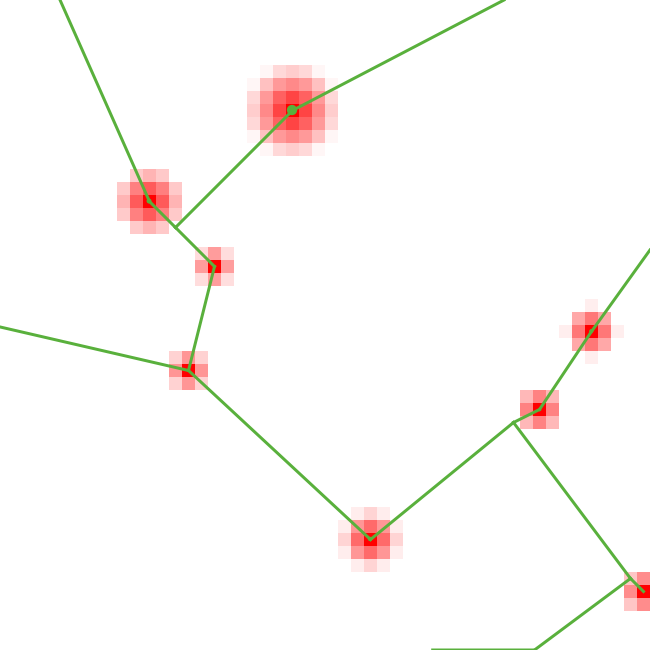
\includegraphics[width=0.35\textwidth]{figures/example_synthsetup}}\hspace{0.1cm}
%\frame{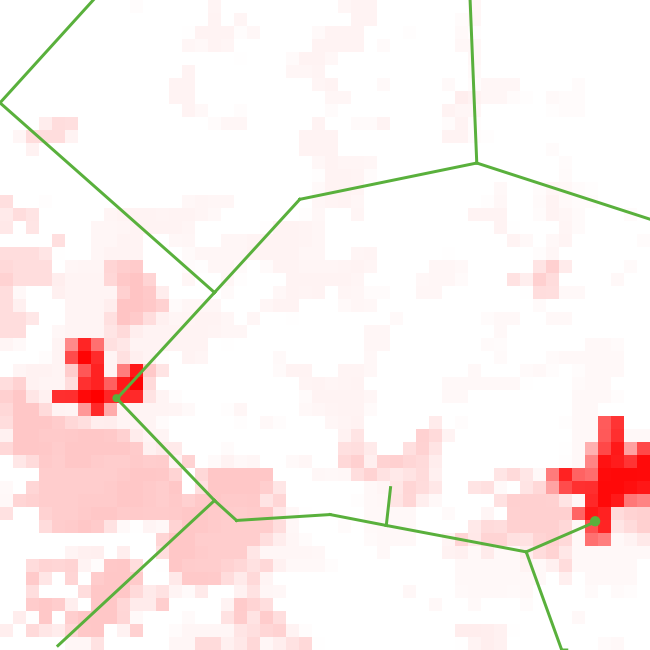
\includegraphics[width=0.35\textwidth]{figures/example-realsetup}}
%
%\textbf{Stopping conditions: } fixed final time; fixed total population; fixed network size.
%
%}
%
%
%\sframe{Calibration Method}{
%
%
%% The model is calibrated at the first order (indicators of urban form and network measures) and at the second order (correlations) with Eurostat population grid coupled with street network from OpenStreetMap through the following workflow: indicators (Moran index, mean distance, hierarchy, entropy for morphology, mean path length, centralities, performance for network) are computed on real areas of width 50km for all Europe (what corresponds to the typical scale of processes the model includes); parameter space of the model is explored using grid computing (with OpenMole model exploration software), from simple synthetic initial configurations (few connected punctual settlements), computing indicators on final simulated configurations;  among candidate parameters for given contiguous (in space and indicator space) real areas on which correlations can be computed, the one with the closest correlation matrix computed on repetitions is chosen.
%
%
%
%\begin{itemize}
%	\item Brute force exploration of a LHS sampling, 10 repetitions of the model for each parameter point.
%	\item For each simulated point, closest in indicator space (euclidian distance for normalized indicators) among real points are selected.
%	\item Among these, point with lowest distance to correlation matrix are taken.
%\end{itemize}
%
%
%}
%
%\sframe{Calibration : optimal points}{
%
%\centering
%
%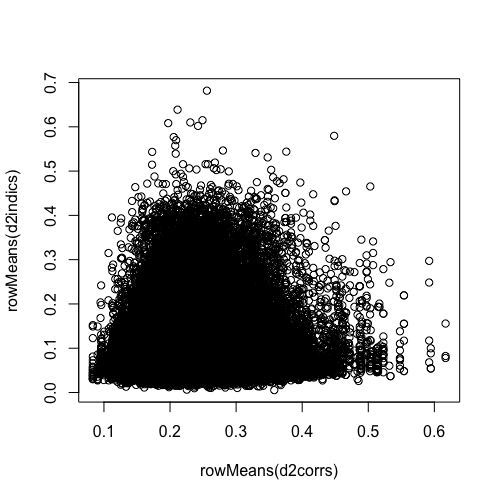
\includegraphics[width=0.45\textwidth]{figures/dists_pareto_i1}
%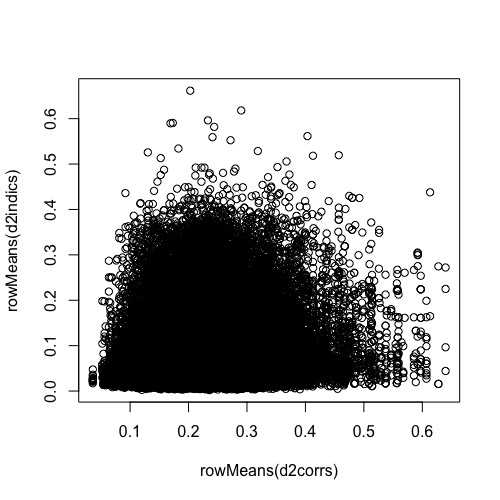
\includegraphics[width=0.45\textwidth]{figures/dists_pareto_i10}
%
%\footnotesize\textit{Pareto plots of distance to indicators and distance to correlation matrices, for a given simulated configuration and all real points.}
%
%}
%
%
%
%\sframe{Causality regimes: clustering}{
%
%\centering
%
%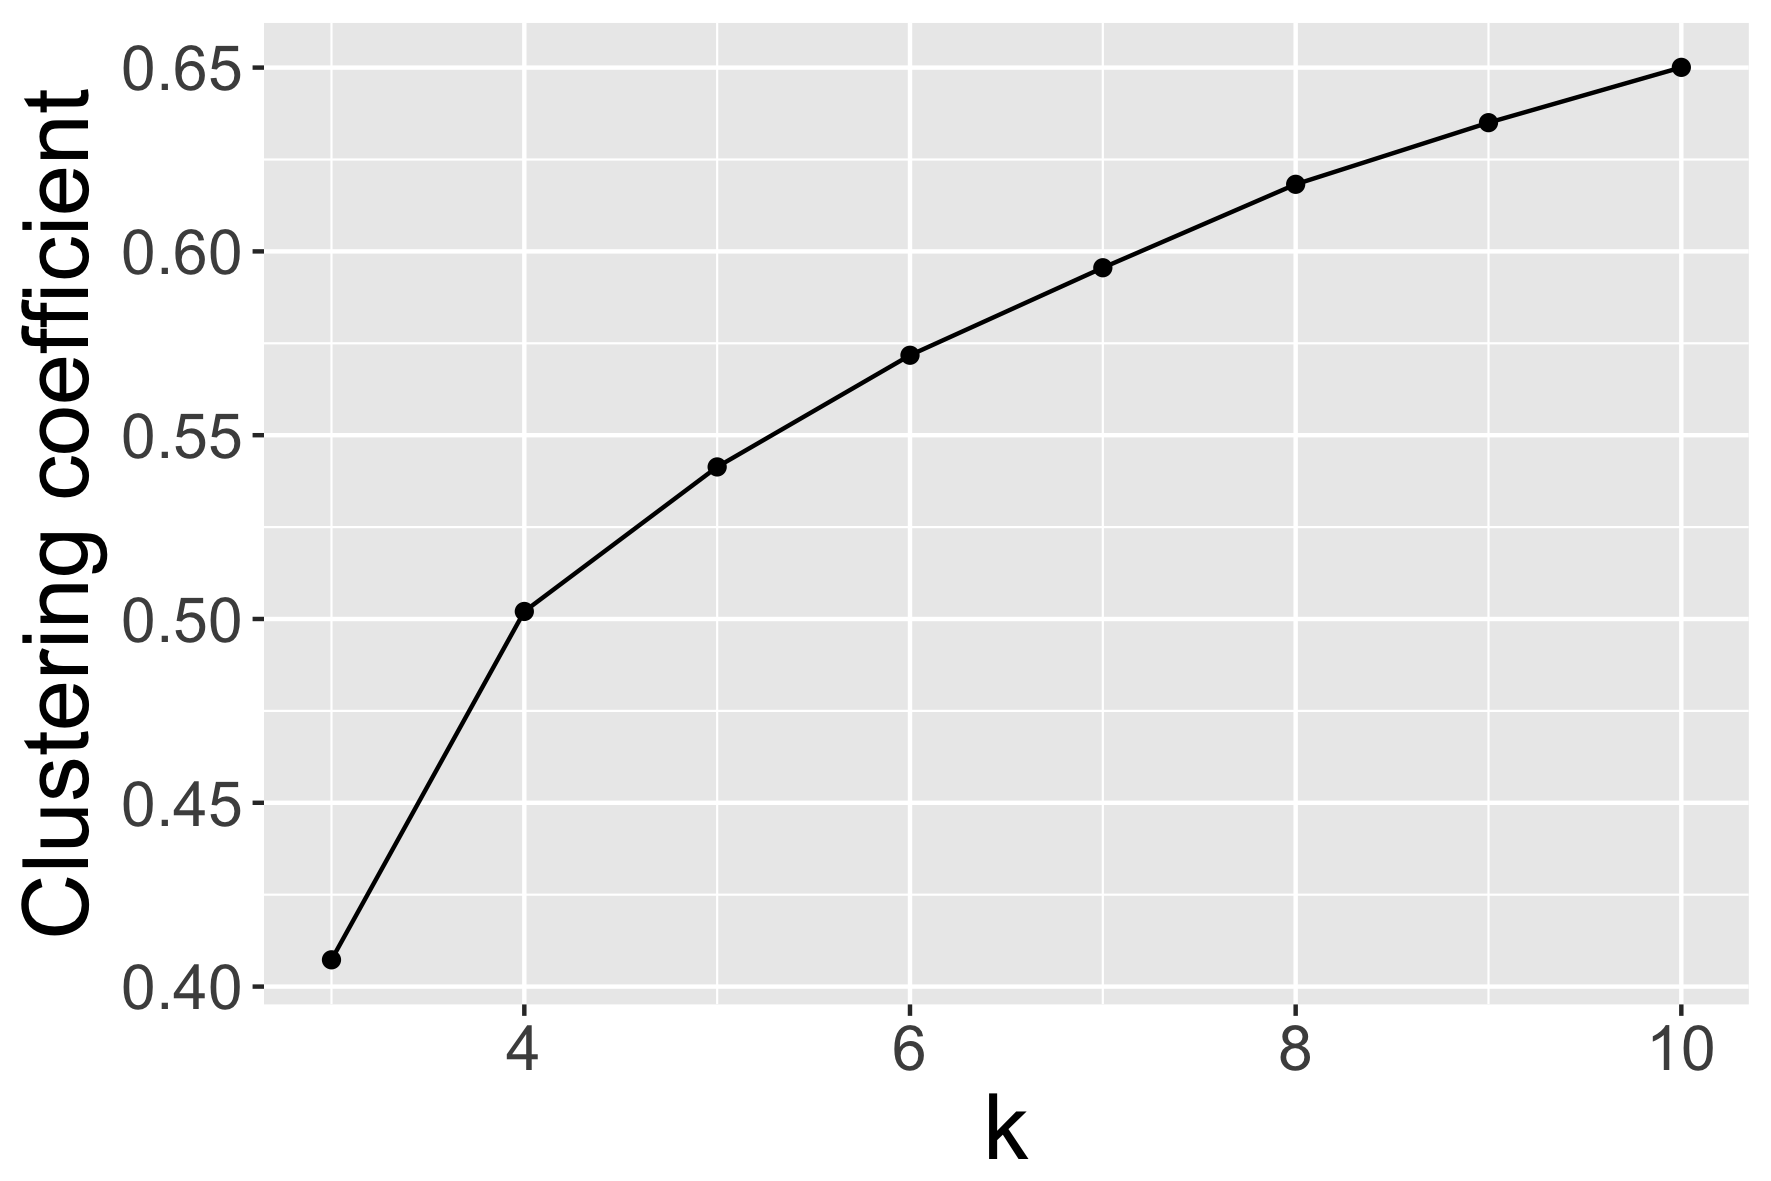
\includegraphics[width=0.48\textwidth]{figures/clustcoef}
%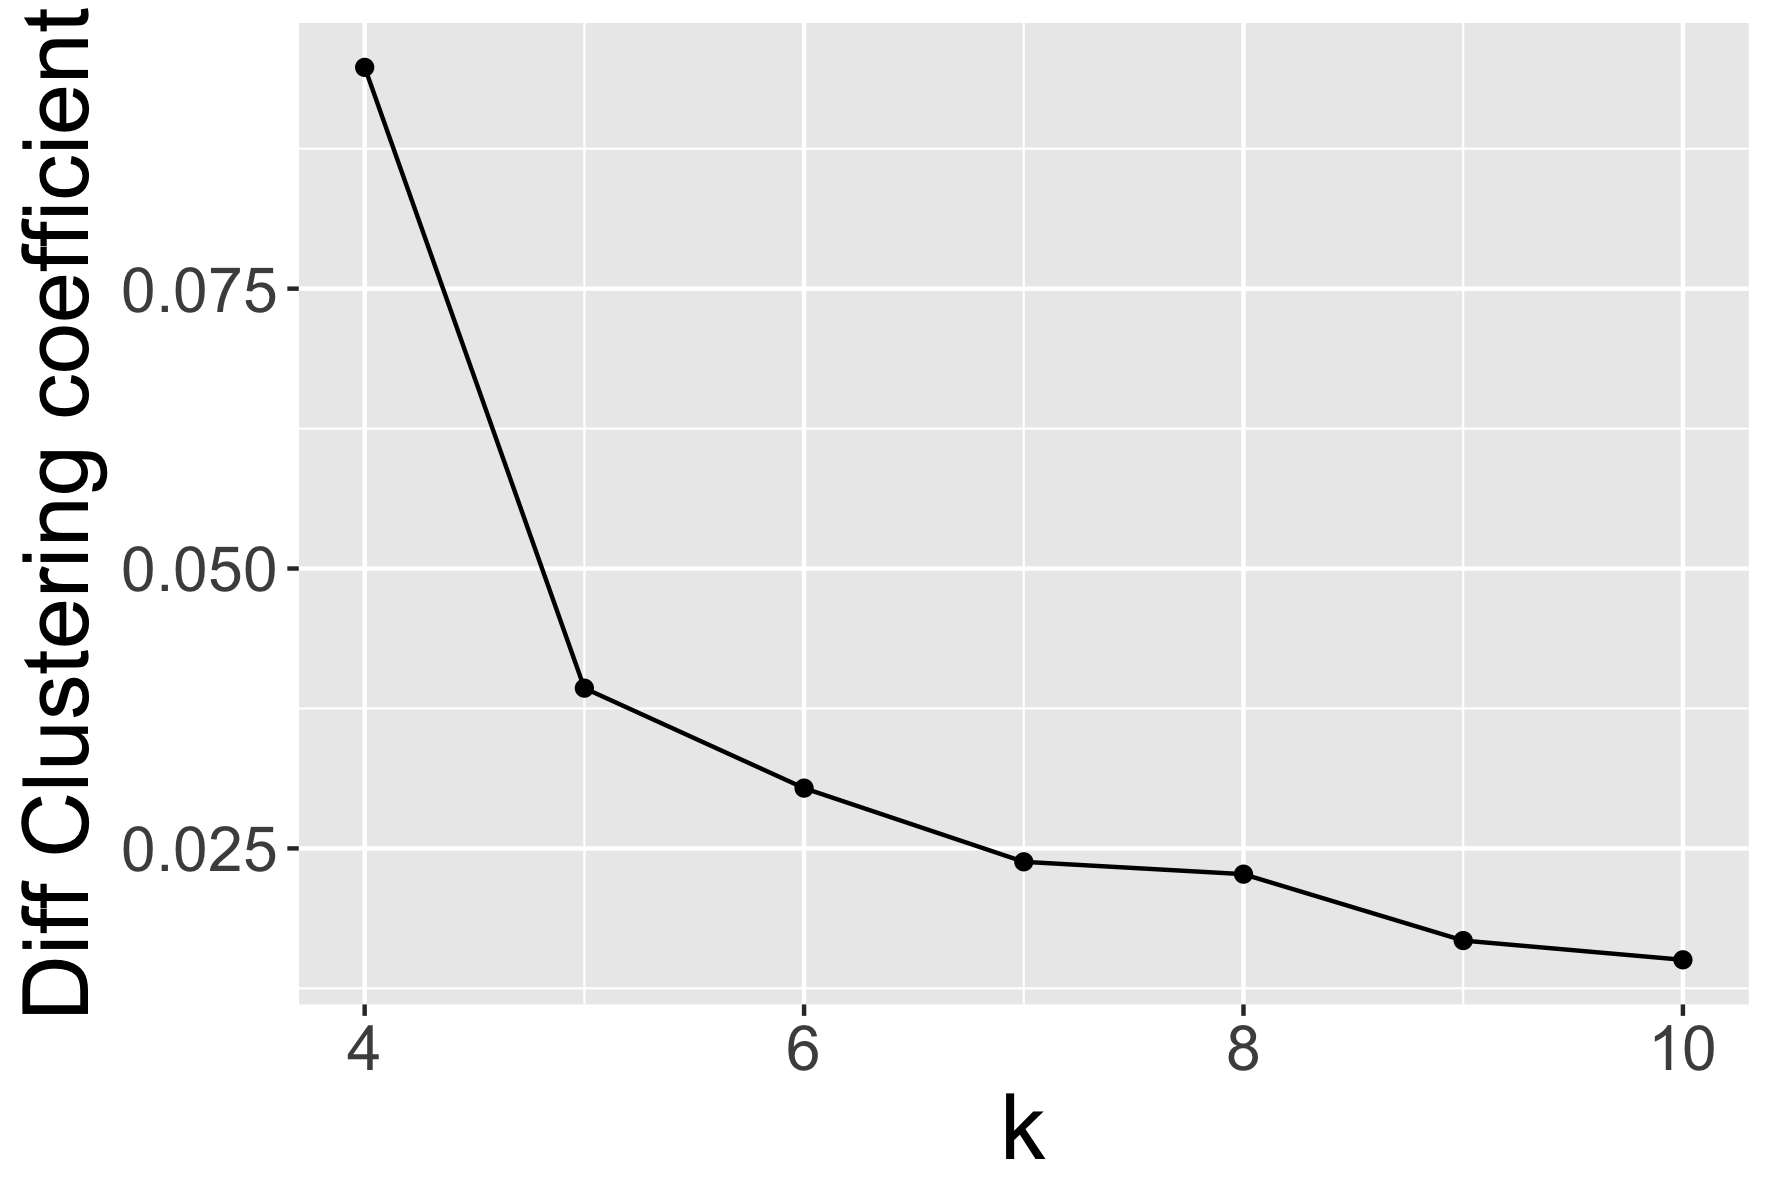
\includegraphics[width=0.48\textwidth]{figures/diffclustcoef}
%
%\medskip
%
%\footnotesize\textit{Clustering coefficient (left) and its derivative (right) as a function of number of clusters}
%
%}
%
%
%
%







\end{document}







